%%%%%%%%%%%%%%%%%%%%%%%%%%%%%%%%%%%%%%%%%%%%%%%%%%%%%%%%%%%%%%
\section{Resultados e conclusões}
%%%%%%%%%%%%%%%%%%%%%%%%%%%%%%%%%%%%%%%%%%%%%%%%%%%%%%%%%%%%%%

%%%%%%%%%%%%%%%%%%%%%%%%%%%%%%%%%%%%%%%%%%%%%%%%%%%%%%%%%%%%%%
\subsection{Resultados e discusões}
%%%%%%%%%%%%%%%%%%%%%%%%%%%%%%%%%%%%%%%%%%%%%%%%%%%%%%%%%%%%%%

%%%%%%%%%%%%%%%%%%%%%%%%%%%%%%%%%%%%%%%%%%%%%%%%%%%%%%%%%%%%%%
\begin{frame}{Softwares utilizados e estrutura do código}
\begin{itemize}
    \item Calculo dos termos fonte foram realizados através do software Mathematica \cite{Mathematica};
    \item O código foi implementado em \textit{Fortran77};
    \item Pós processamentos foram realizados utilizando MatLab; 
\end{itemize}
\end{frame}

%%%%%%%%%%%%%%%%%%%%%%%%%%%%%%%%%%%%%%%%%%%%%%%%%%%%%%%%%%%%%%
\begin{frame}{Softwares utilizados e estrutura do código}
\begin{figure}[htb]
 \centering
 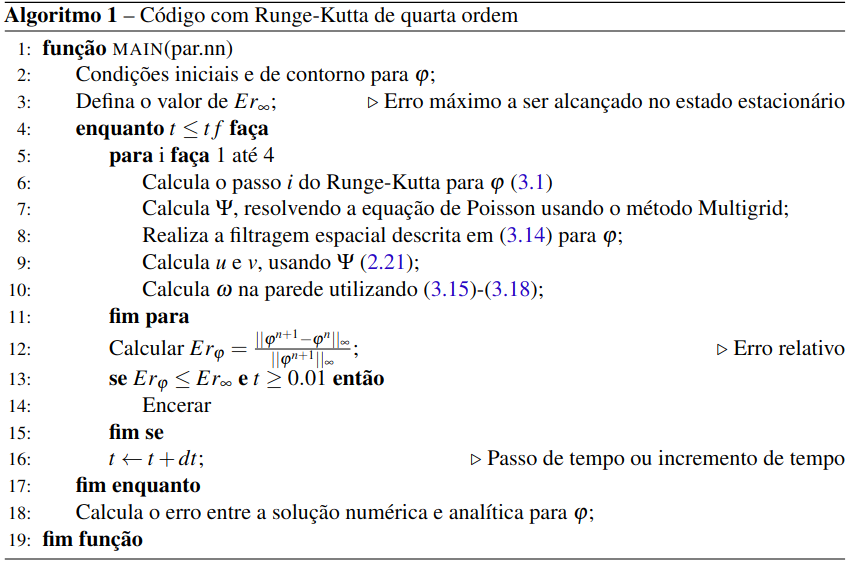
\includegraphics[scale=0.55]{Figures/pseudo.png}
 \caption*{}
\end{figure}
\end{frame}

%%%%%%%%%%%%%%%%%%%%%%%%%%%%%%%%%%%%%%%%%%%%%%%%%%%%%%%%%%%%%%
\begin{frame}{Softwares utilizados e estrutura do código}
A norma $k$ para o termo de erro $e$, definido como:
\begin{align}
    &\left \|e\right \|_{k}=\left(\Delta x \Delta y \sum_{i=1}^{N_{1}}\sum_{j=1}^{N_{2}} \left |e\right |_{i,j}^{k}\right)^{1/k}, \label{norm_k}
\end{align}

Para determinar a ordem de convergência numérica, representada por $p$, adotamos o procedimento descrito por \cite{leveque2007finite}:
\begin{equation}\label{log_p} 
    p \approx \frac{\log\left(\frac{e_{i}}{e_{i+1}}\right)}{\log\left(\frac{h_{i}}{h_{i+1}}\right)}. 
\end{equation}
\end{frame}

%%%%%%%%%%%%%%%%%%%%%%%%%%%%%%%%%%%%%%%%%%%%%%%%%%%%%%%%%%%%%%
\begin{frame}{Bateria de testes}
\begin{table}[h]
    \caption{Parâmetros utilizados para os testes realizados}\label{tab_test_cases}
    \begin{tabular}{c|cccccc}
        \toprule
        \textbf{Modelo} & $\operatorname{Re}$ & $\beta_{nn}$ & $\operatorname{Wi}$ & $\alpha_{G}$ & $\epsilon$ & $\xi$ \\ \midrule
        \textbf{UCM} & 1, 10, 100, 400, 1000 & 0 & 1, 5, 10 & 0 & 0 & 0 \\ \midrule
        \textbf{Oldroyd-B} & 1, 10, 100, 400, 1000 & 0.1, 0.5, 0.9, 1 & 1, 5, 10 & 0 & 0 & 0 \\ \midrule
        \textbf{Giesekus} & 1, 10, 100, 400, 1000 & 0.1, 0.5, 0.9, 1 & 1, 5, 10 & 0.1, 0.5, 0.85 & 0 & 0 \\ \midrule
        \textbf{LPTT} & 1, 10, 100, 400, 1000 & 0.1, 0.5, 0.9, 1.0 & 1, 5, 10 & 0 & 0.5, 1 & 0.1, 0.5 \\ \bottomrule
    \end{tabular}
\end{table}
\end{frame}

%%%%%%%%%%%%%%%%%%%%%%%%%%%%%%%%%%%%%%%%%%%%%%%%%%%%%%%%%%%%%%
\begin{frame}{Domínio computacional}
Para todos os casos teste, considera-se o domínio $\Omega = [0,L]\times[0,H] = [0,1]\times[0,1]$, como ilustrado abaixo:
\begin{figure}[H]
        \centering
	\caption{Domínio computacional}\label{fig:domain}
        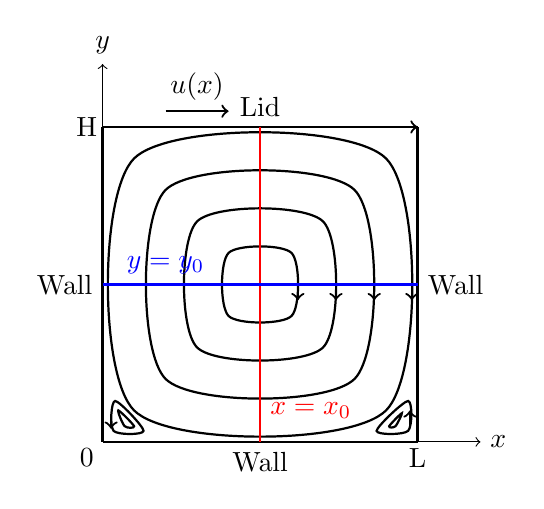
\begin{tikzpicture}[scale=4]
            % Eixos x e y
            \draw[->] (0,0) -- (1.2,0) node[right] {$x$};
            \draw[->] (0,0) -- (0,1.2) node[above] {$y$};
            % Desenhando o quadrado do domínio
            \draw (0,0) rectangle (1,1);
            % Desenho da tampa (lid)
            \draw[->, thick] (0,1) -- (1,1) node[midway, above] {Lid};
            \draw[-, thick]  (0,0) -- (1,0) node[midway, below] {Wall};
            \draw[-, thick]  (0,0) -- (0,1) node[midway, left] {Wall};
            \draw[-, thick]  (1,0) -- (1,1) node[midway, right] {Wall};
            \draw[->, thick] (0.2,1.05) -- (0.4,1.05) node[midway, above] {$u(x)$};
            % Outras anotações
            \node at (-0.05,-0.05) {0};
            \node at (1,-0.05) {L};
            \node at (-0.05,1) {H};
            % Vortice central
            \draw[thick] plot[smooth cycle] coordinates {(0.1,0.9) (0.9,0.9) (0.9,0.1) (0.1,0.1)};
            \draw[thick] plot[smooth cycle] coordinates {(0.2,0.8) (0.8,0.8) (0.8,0.2) (0.2,0.2)};
            \draw[thick] plot[smooth cycle] coordinates {(0.3,0.7) (0.7,0.7) (0.7,0.3) (0.3,0.3)};
            \draw[thick] plot[smooth cycle] coordinates {(0.4,0.6) (0.6,0.6) (0.6,0.4) (0.4,0.4)};
            \draw[->, thick] (0.62,0.5) -- (0.62,0.45);
            \draw[->, thick] (0.741,0.5) -- (0.741,0.45);
            \draw[->, thick] (0.8625,0.5) -- (0.8625,0.45);
            \draw[->, thick] (0.982,0.5) -- (0.982,0.45);
            % Vortice inferrior esquerdo
            \draw[thick] plot[smooth cycle] coordinates {(0.07,0.05) (0.05,0.1) (0.1,0.05)};
            \draw[thick] plot[smooth cycle] coordinates {(0.035,0.035) (0.04,0.13) (0.13,0.035)};
            \draw[->, thick] (0.027,0.09) -- (0.027,0.042);
            % Vortice inferior direito
            \draw[thick] plot[smooth cycle] coordinates {(0.93,0.05) (0.95,0.091) (0.91,0.05)};
            \draw[thick] plot[smooth cycle] coordinates {(0.97,0.035) (0.97,0.13) (0.87,0.035)};
            \draw[->, thick] (0.976,0.05) -- (0.976,0.1);
            % Linha vertical em x = 0.5
            \draw[red, thick] (0.5, 0) -- (0.5, 1) node[pos=0.1, right] {$x = x_0$};
            % Linha horizontal em y = 0.5
            \draw[blue, thick] (0, 0.5) -- (1, 0.5) node[pos=0.2, above] {$y = y_0$};
        \end{tikzpicture}
\end{figure}
\end{frame}

%%%%%%%%%%%%%%%%%%%%%%%%%%%%%%%%%%%%%%%%%%%%%%%%%%%%%%%%%%%%%%
\begin{frame}{Soluções Manufaturadas}
    \centering
    \captionsetup{justification=centering}
    \captionof{figure}{Soluções manufaturadas no regime de estado estacionário para o campo de velocidades $(\overline{u},\tilde{v})$, considerando $a = 0.05$}
    \label{fig:sol_manufaturadas_1}
    \begin{minipage}{0.48\textwidth}
        \centering
        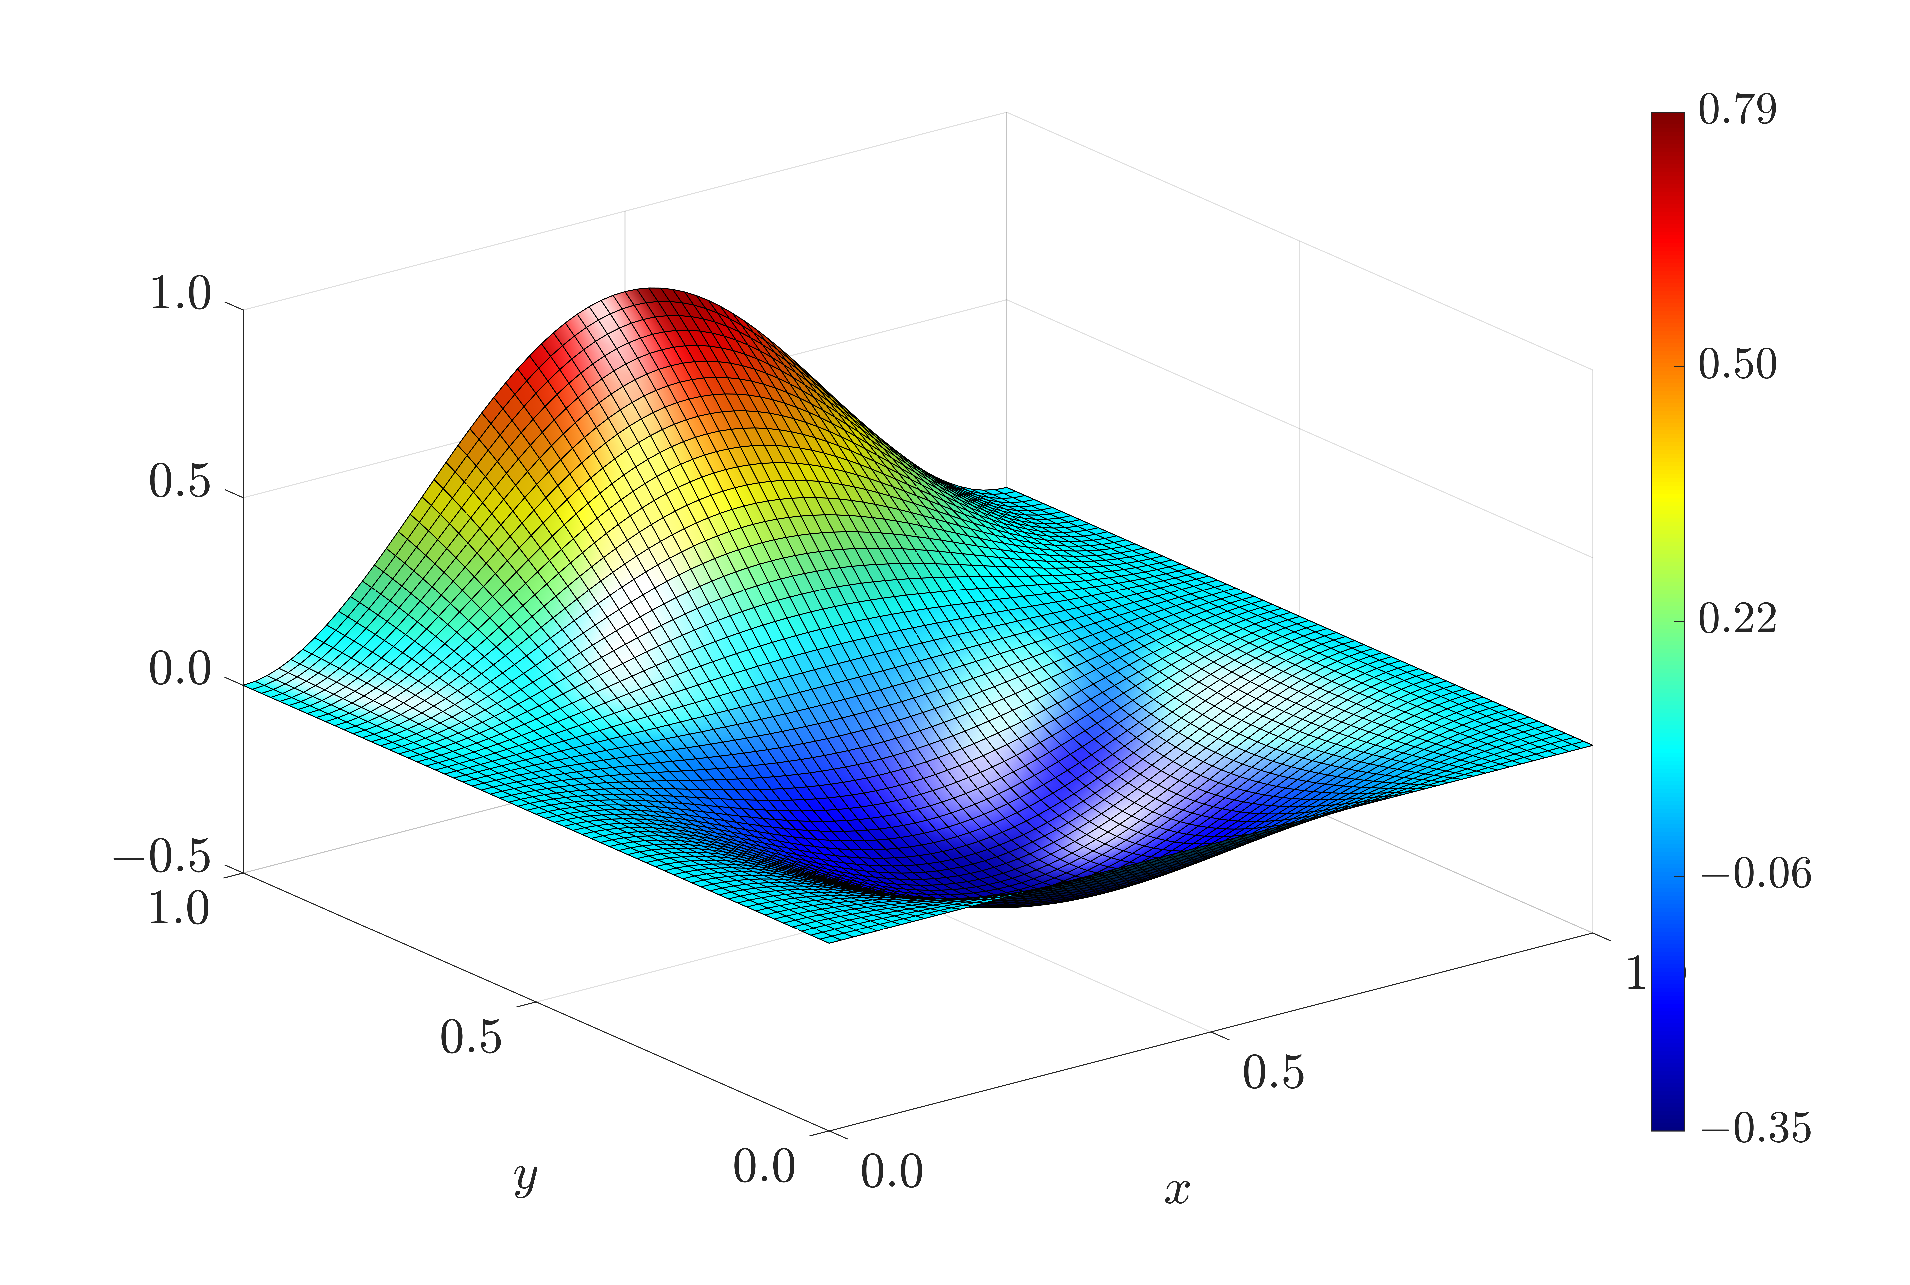
\includegraphics[width=\textwidth]{Figures/Exact_Surf_NormErr_2nd_Betann_0.1_Re_1_Wi_1_epsilon_0_xi_0_alphaG_0_Dt_1e-06_at_0.05_tipsim_1_MMS_12_U.eps}
        \captionof{subfigure}{$\overline{u}$}
        \label{fig_solexauCase1}
    \end{minipage}
    \hfill
    \begin{minipage}{0.48\textwidth}
        \centering
        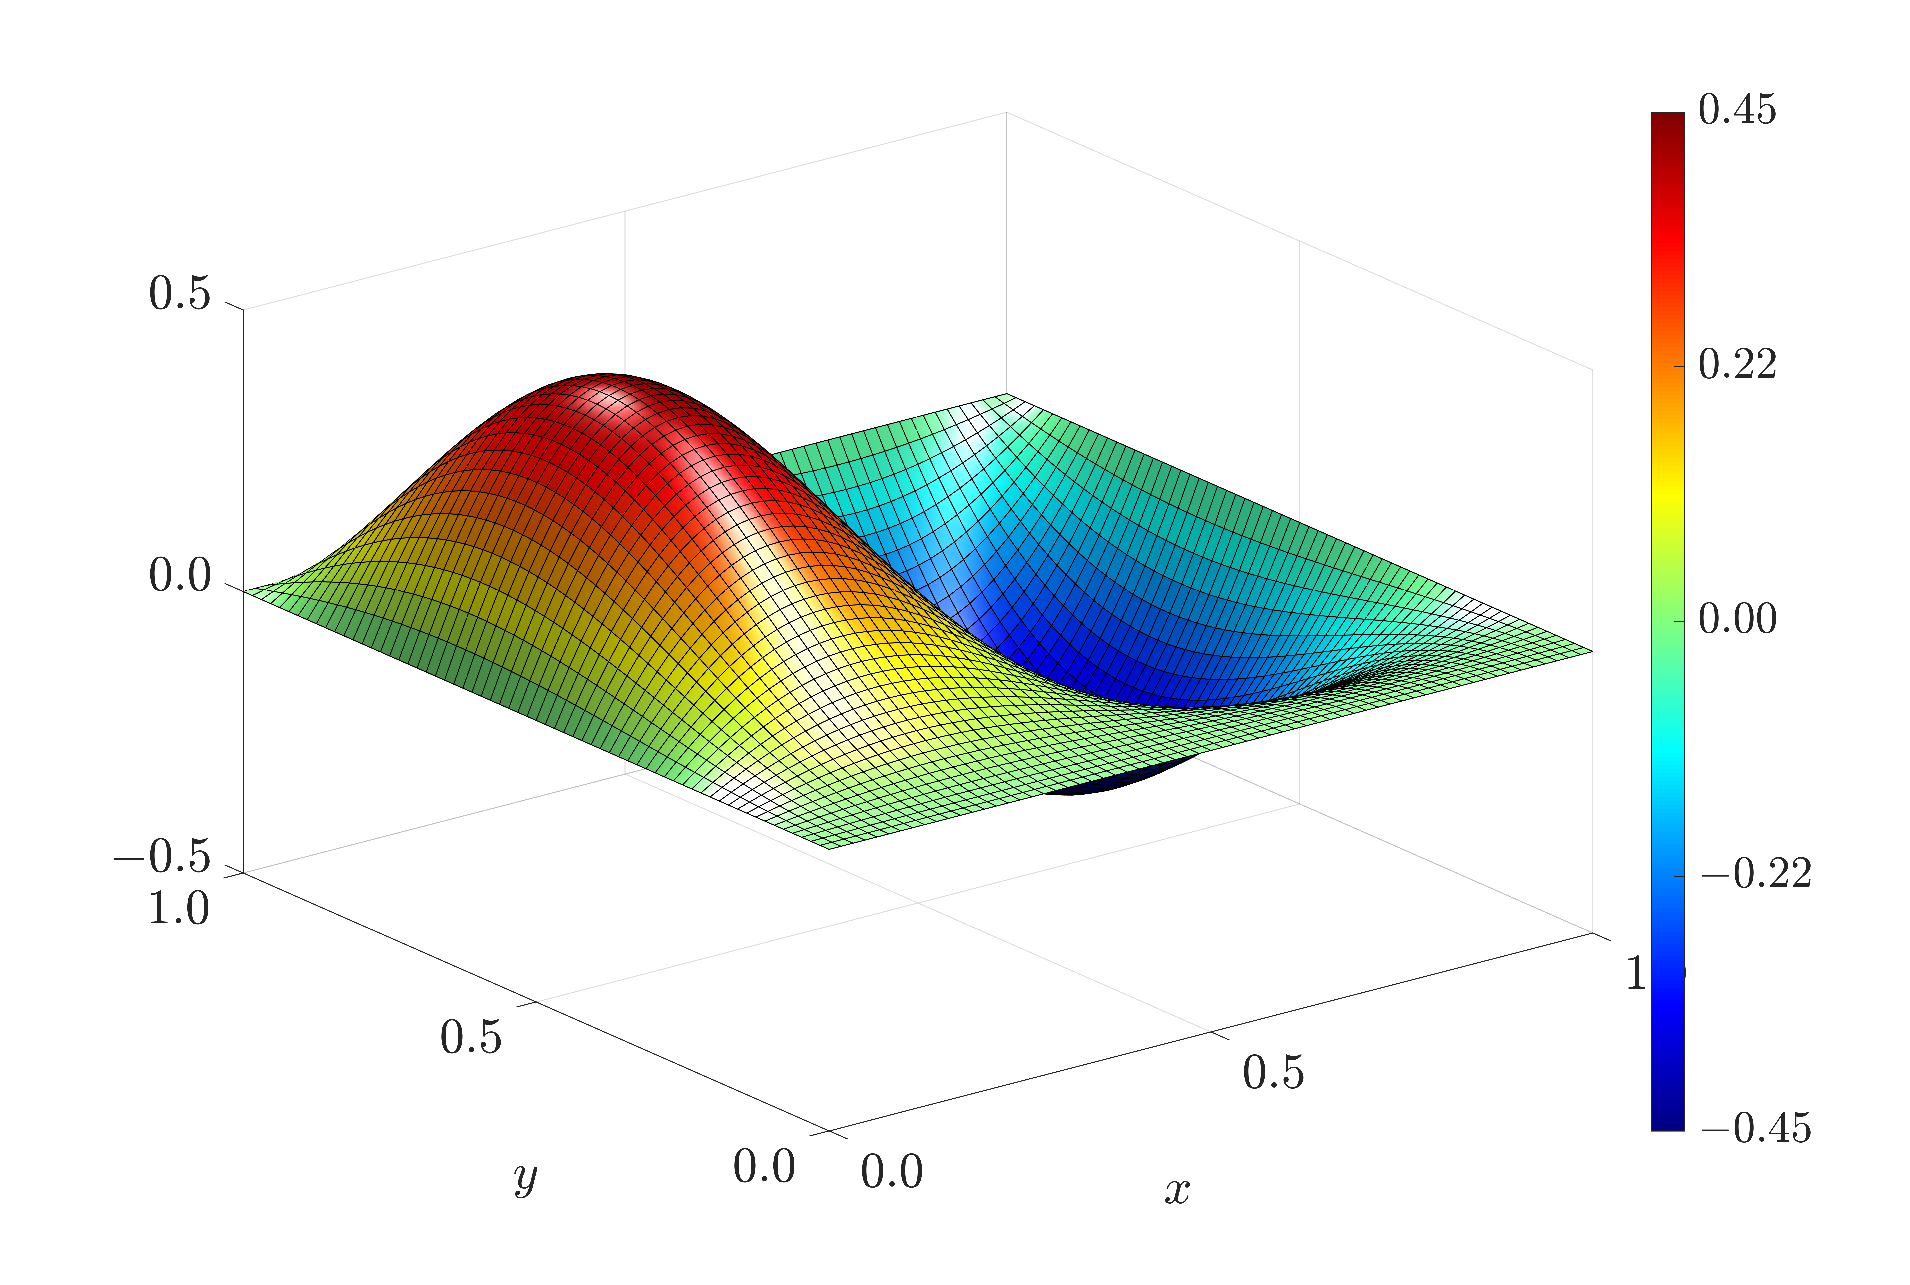
\includegraphics[width=\textwidth]{Figures/Exact_Surf_NormErr_2nd_Betann_0.1_Re_1_Wi_1_epsilon_0_xi_0_alphaG_0_Dt_1e-06_at_0.05_tipsim_1_MMS_12_V.eps}
        \captionof{subfigure}{$\widetilde{v}$}
        \label{fig_solexavCase1}
    \end{minipage}
\end{frame}

%%%%%%%%%%%%%%%%%%%%%%%%%%%%%%%%%%%%%%%%%%%%%%%%%%%%%%%%%%%%%%
\begin{frame}{Soluções Manufaturadas}
    \centering
    \captionsetup{justification=centering}
    \captionof{figure}{Soluções manufaturadas no regime de estado estacionário
    para a vorticidade $(\tilde{\omega_{z}})$ e função de corrente $(\tilde{\psi})$, considerando $a = 0.05$}
    \label{fig:sol_manufaturadas_2}
    \begin{minipage}{0.48\textwidth}
        \centering
        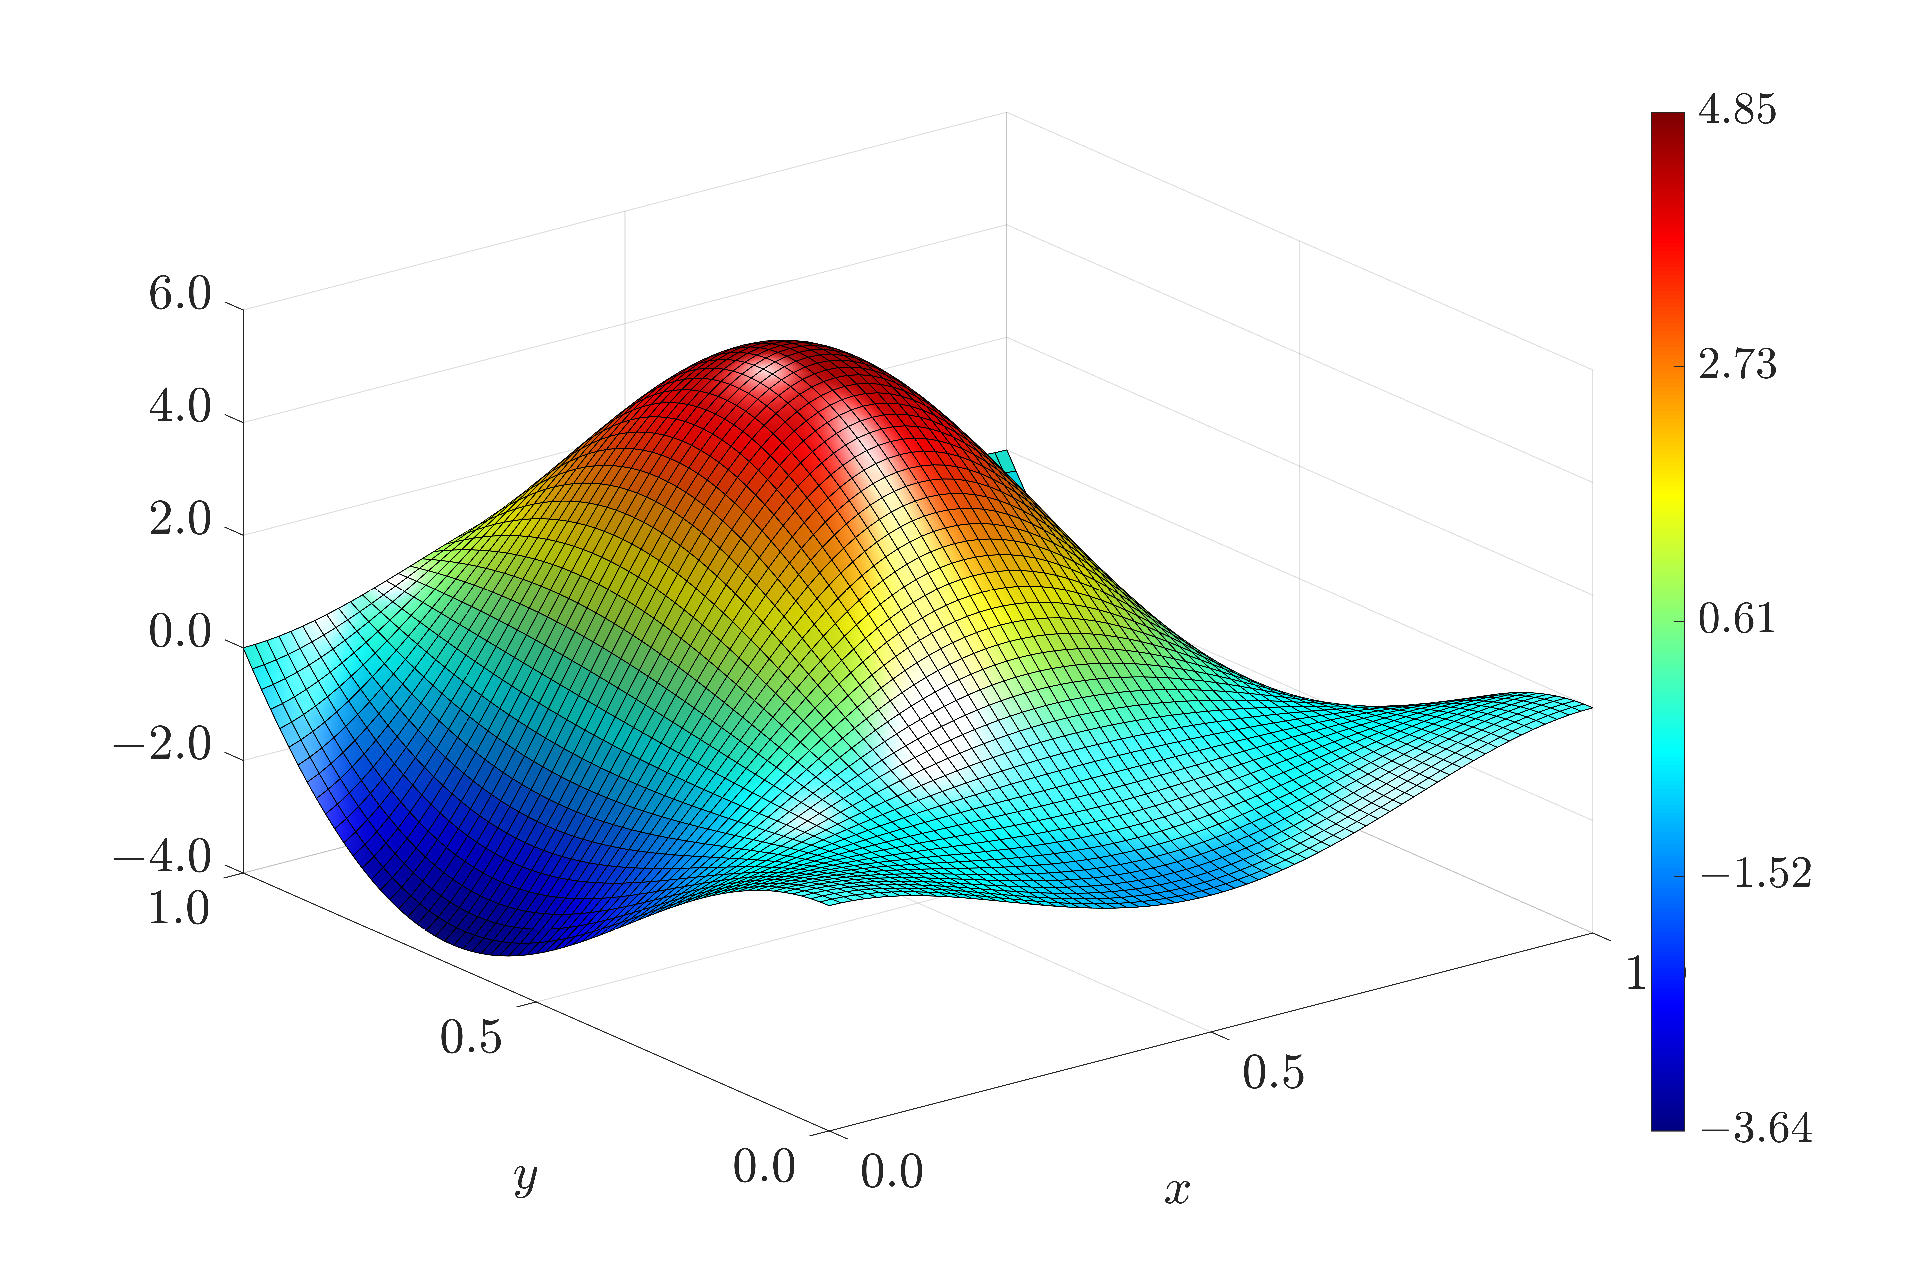
\includegraphics[width=\textwidth]{Figures/Exact_Surf_NormErr_2nd_Betann_0.1_Re_1_Wi_1_epsilon_0_xi_0_alphaG_0_Dt_1e-06_at_0.05_tipsim_1_MMS_12_Wz.eps}
        \captionof{subfigure}{$\widetilde{\omega_{z}}$}
        \label{fig_solexawzCase1}
    \end{minipage}
    \hfill
    \begin{minipage}{0.48\textwidth}
        \centering
        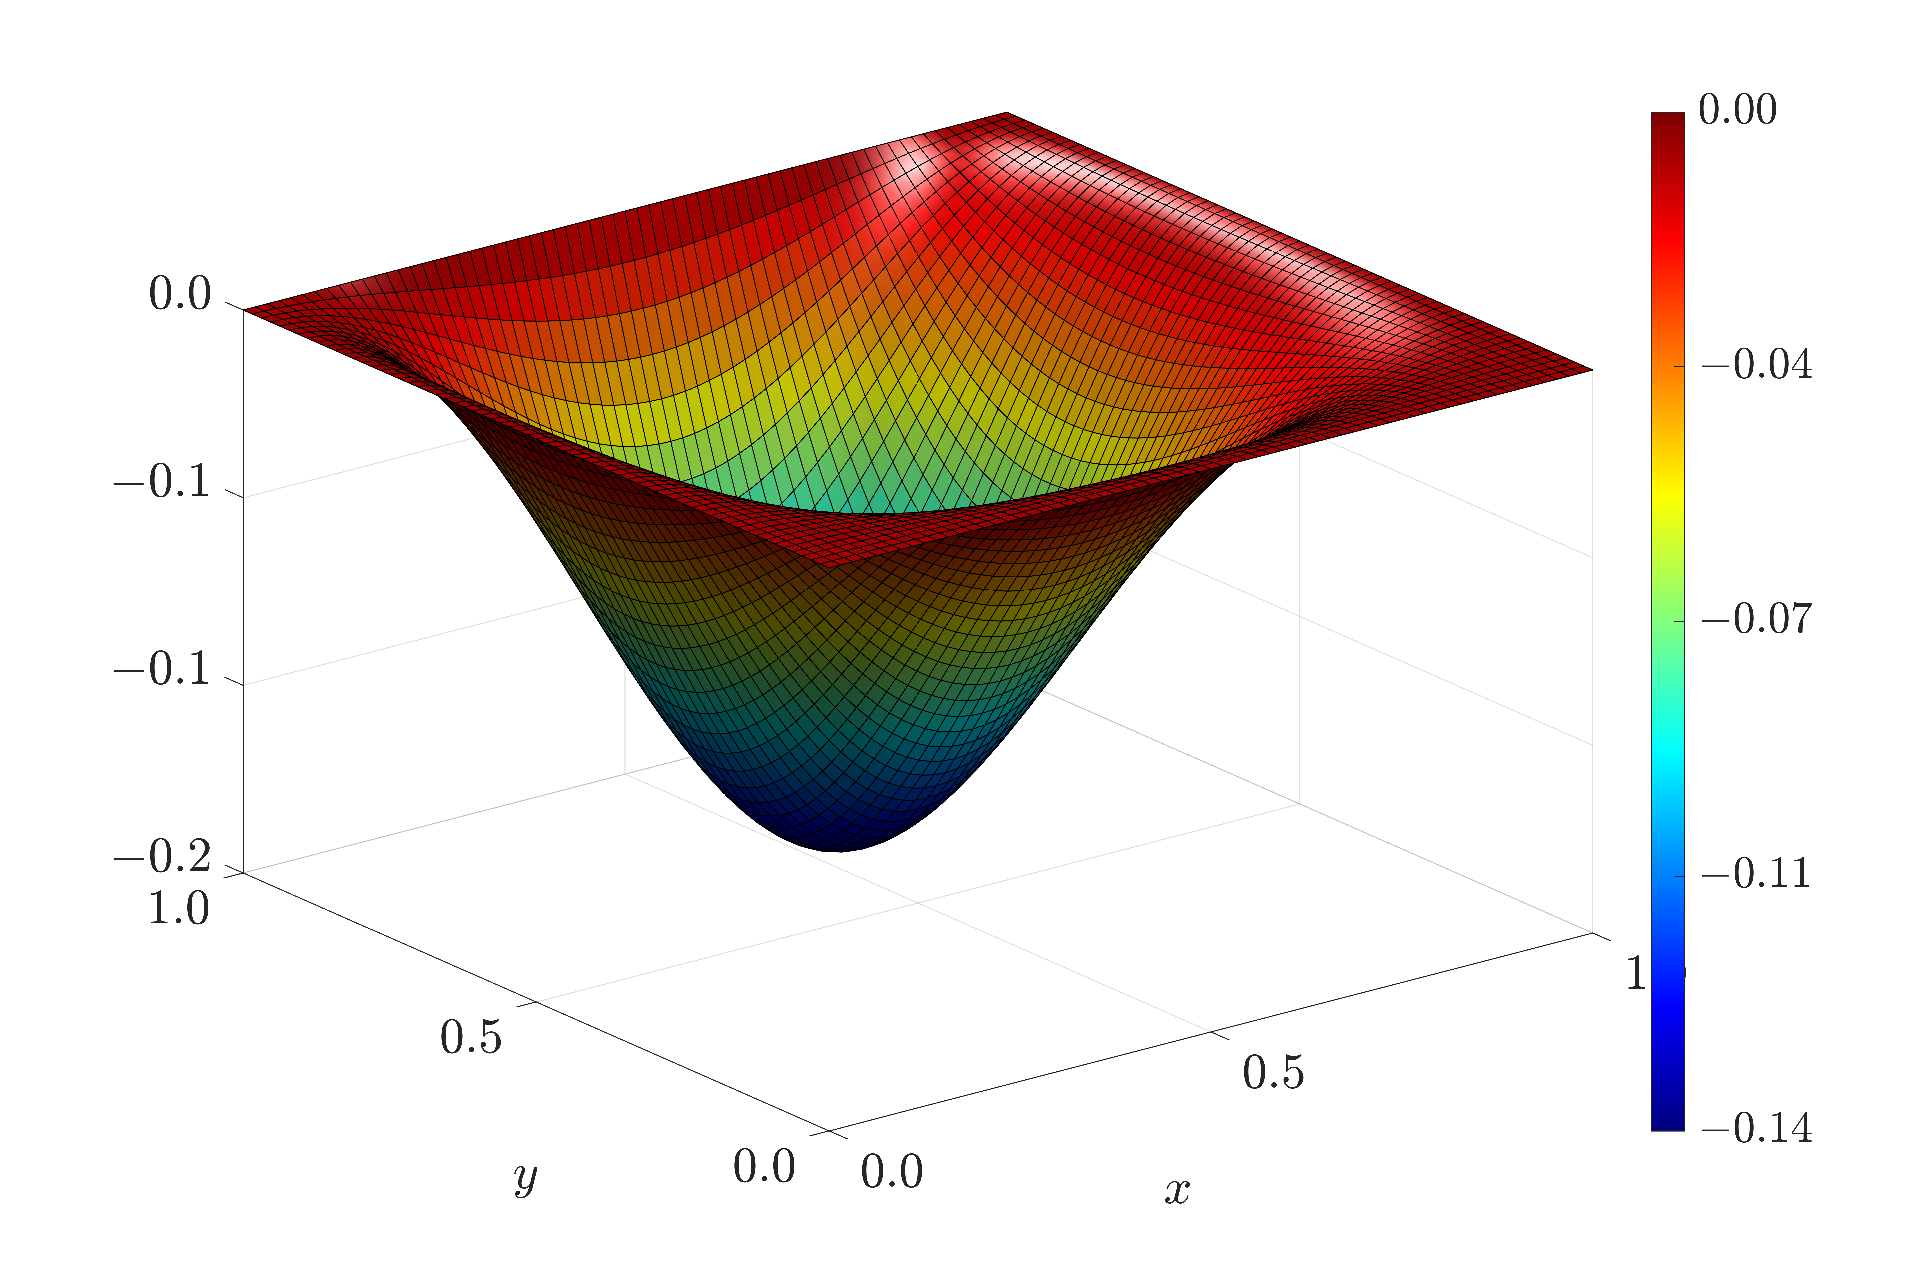
\includegraphics[width=\textwidth]{Figures/Exact_Surf_NormErr_2nd_Betann_0.1_Re_1_Wi_1_epsilon_0_xi_0_alphaG_0_Dt_1e-06_at_0.05_tipsim_1_MMS_12_Psi.eps}
        \captionof{subfigure}{$\widetilde{\psi}$}
        \label{fig_solexapsiCase1}
    \end{minipage}
\end{frame}

%%%%%%%%%%%%%%%%%%%%%%%%%%%%%%%%%%%%%%%%%%%%%%%%%%%%%%%%%%%%%%
\begin{frame}{Soluções Manufaturadas}
    \centering
    \captionsetup{justification=centering}
    \captionof{figure}{Soluções manufaturadas no regime de estado estacionário para os tensores, considerando $\beta_{nn}=0.1$ e $a = 0.05$}
    \label{fig:sol_manufaturadas_3}
    \begin{minipage}{0.31\textwidth}
        \centering
        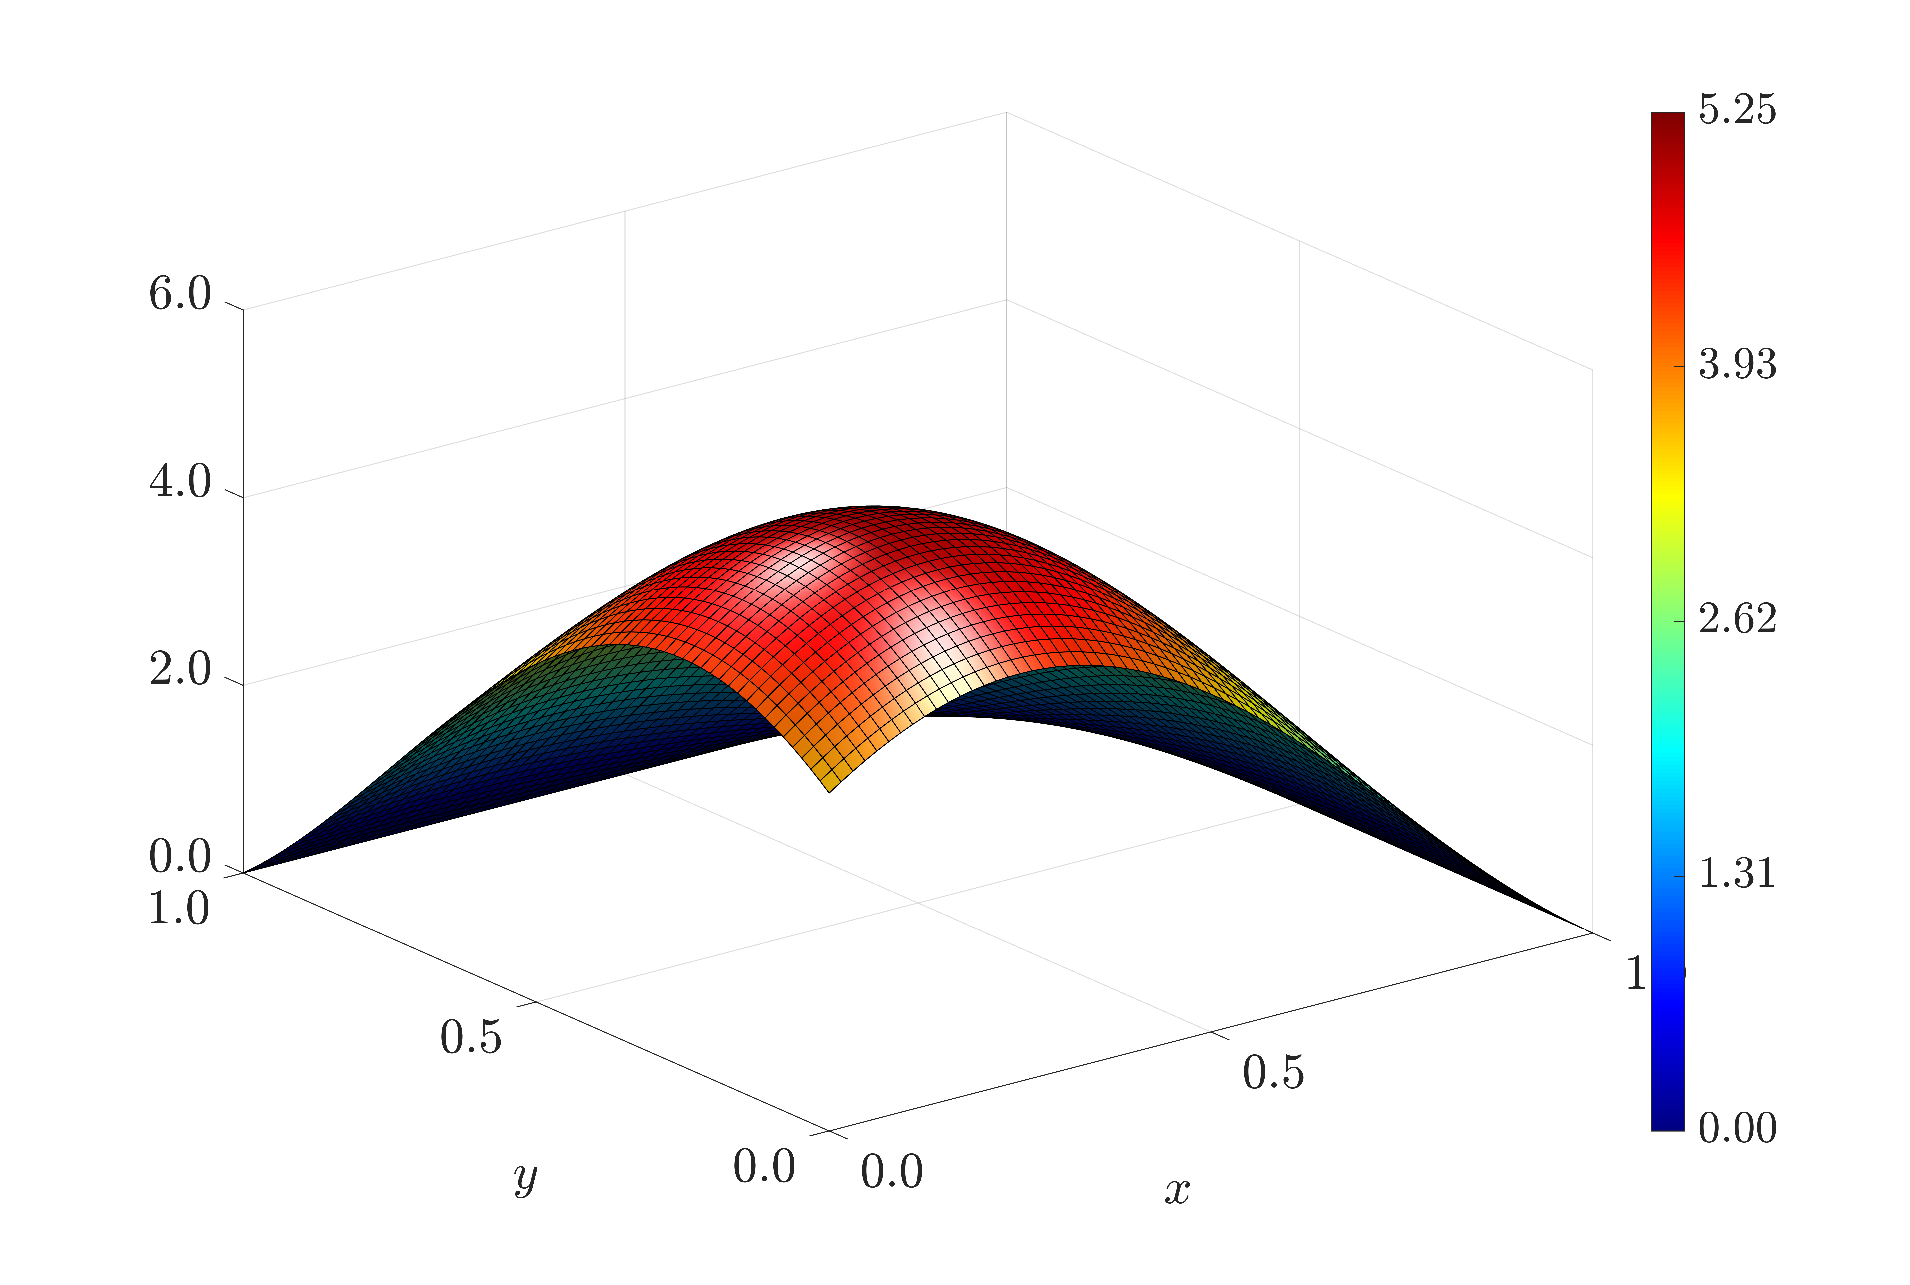
\includegraphics[width=\textwidth]{Figures/Exact_Surf_NormErr_2nd_Betann_0.1_Re_1_Wi_1_epsilon_0_xi_0_alphaG_0_Dt_1e-06_at_0.05_tipsim_1_MMS_12_Txx.eps}
        \captionof{subfigure}{$\overline{T}_{xx}$}
        \label{fig_solexaTxxCase1}
    \end{minipage}
    \hfill
    \begin{minipage}{0.31\textwidth}
        \centering
        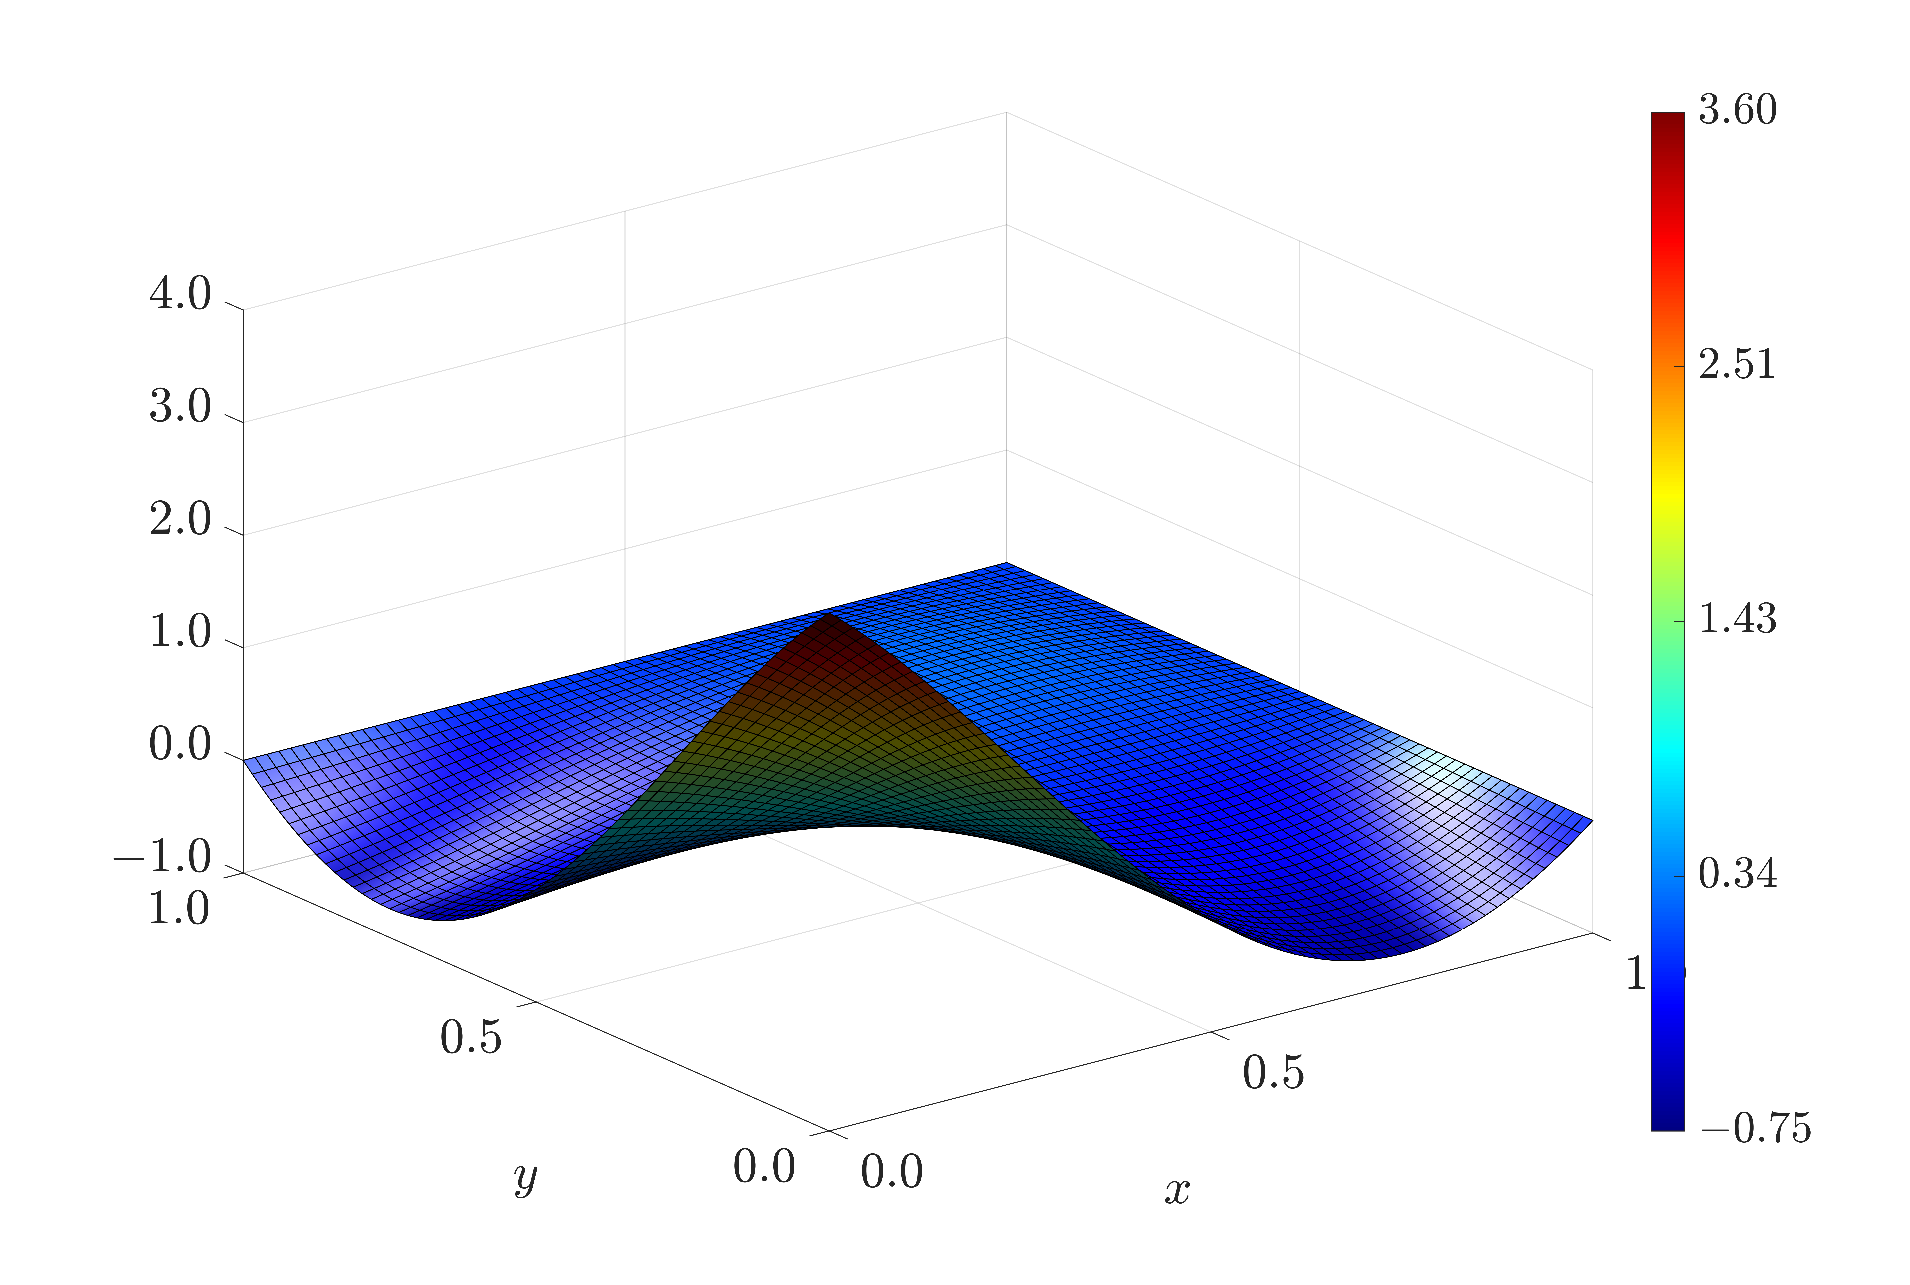
\includegraphics[width=\textwidth]{Figures/Exact_Surf_NormErr_2nd_Betann_0.1_Re_1_Wi_1_epsilon_0_xi_0_alphaG_0_Dt_1e-06_at_0.05_tipsim_1_MMS_12_Txy.eps}
        \captionof{subfigure}{$\overline{T}_{xy}$}
        \label{fig_solexaTxyCase1}
    \end{minipage}
    \hfill
    \begin{minipage}{0.31\textwidth}
        \centering
        \includegraphics[width=\textwidth]{Figures/Exact_Surf_NormErr_2nd_Betann_0.1_Re_1_Wi_1_epsilon_0_xi_0_alphaG_0_Dt_1e-06_at_0.05_tipsim_1_MMS_12_Tyy.eps}
        \captionof{subfigure}{$\overline{T}_{yy}$}
        \label{fig_solexaTyyCase1}
    \end{minipage}
\end{frame}


%%%%%%%%%%%%%%%%%%%%%%%%%%%%%%%%%%%%%%%%%%%%%%%%%%%%%%%%%%%%%%
\begin{frame}{Soluções Manufaturadas}
    \centering
    \captionsetup{justification=centering}
    \captionof{figure}{Soluções manufaturadas no regime de estado estacionário para o campo de velocidades $(\overline{u},\tilde{v})$, considerando $a = 0.05$}
    \label{fig:sol_manufaturadas_11}
    \begin{minipage}{0.48\textwidth}
        \centering
        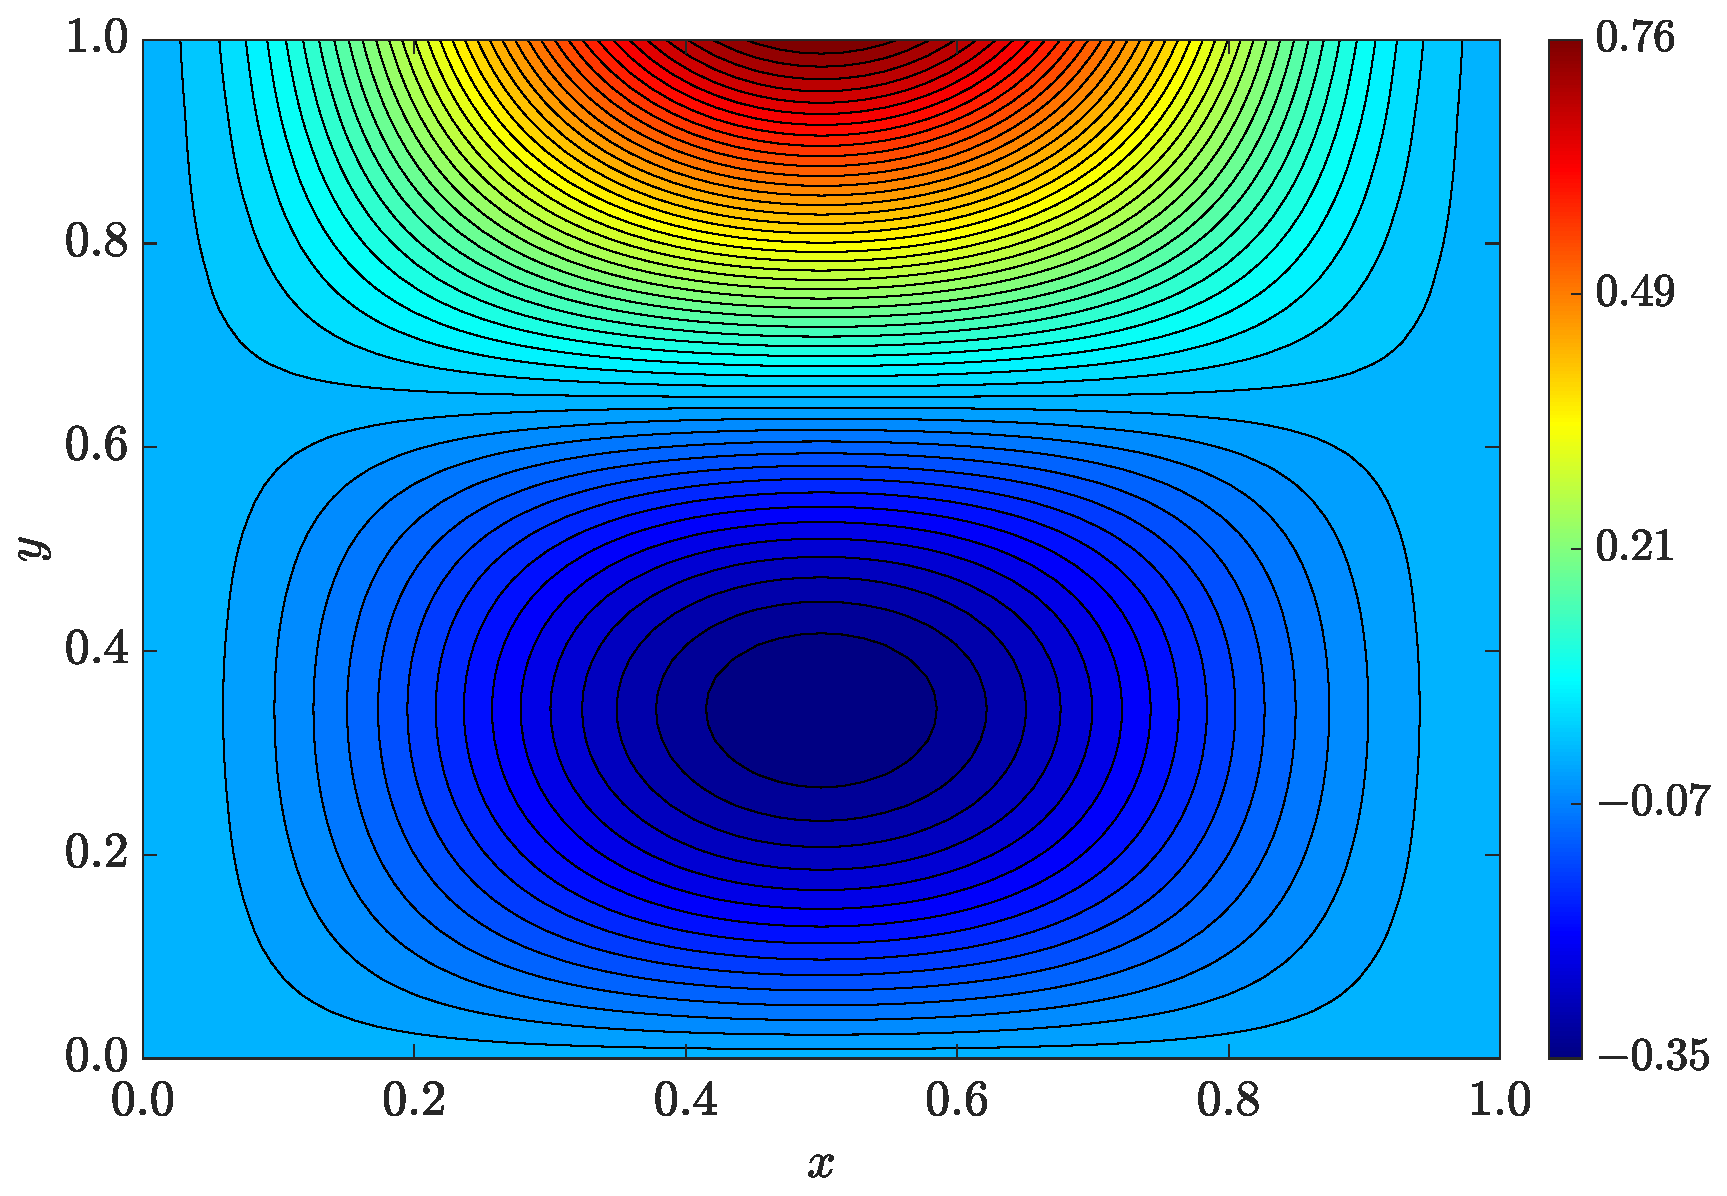
\includegraphics[width=\textwidth]{Figures/Exact_Map_NormErr_2nd_Betann_0.1_Re_1_Wi_1_epsilon_0_xi_0_alphaG_0_Dt_1e-06_at_0.05_tipsim_1_MMS_12_U.eps}
        \captionof{subfigure}{$\overline{u}$}
        \label{fig_solexauCase11}
    \end{minipage}
    \hfill
    \begin{minipage}{0.48\textwidth}
        \centering
        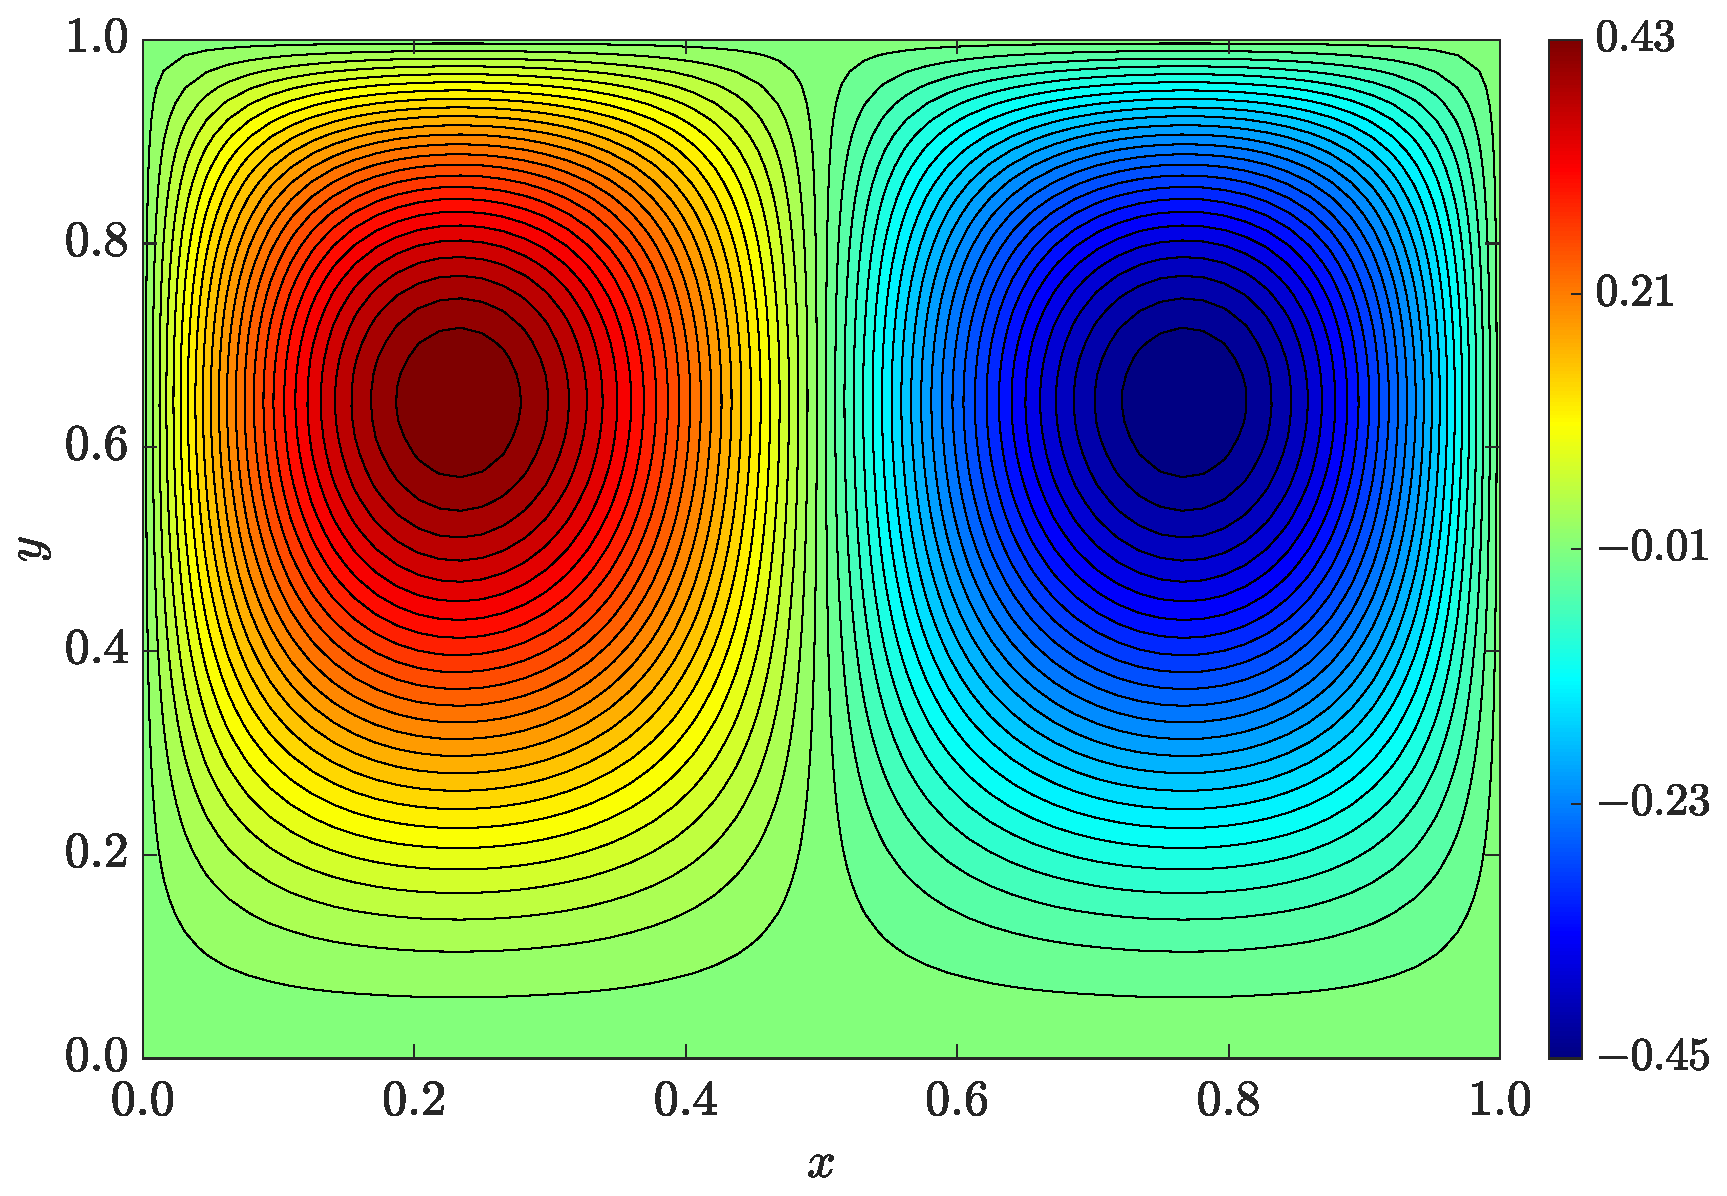
\includegraphics[width=\textwidth]{Figures/Exact_Map_NormErr_2nd_Betann_0.1_Re_1_Wi_1_epsilon_0_xi_0_alphaG_0_Dt_1e-06_at_0.05_tipsim_1_MMS_12_V.eps}
        \captionof{subfigure}{$\widetilde{v}$}
        \label{fig_solexavCase11}
    \end{minipage}
\end{frame}

%%%%%%%%%%%%%%%%%%%%%%%%%%%%%%%%%%%%%%%%%%%%%%%%%%%%%%%%%%%%%%
\begin{frame}{Soluções Manufaturadas}
    \centering
    \captionsetup{justification=centering}
    \captionof{figure}{Soluções manufaturadas no regime de estado estacionário
    para a vorticidade $(\tilde{\omega_{z}})$ e função de corrente $(\tilde{\psi})$, considerando $a = 0.05$}
    \label{fig:sol_manufaturadas_21}
    \begin{minipage}{0.48\textwidth}
        \centering
        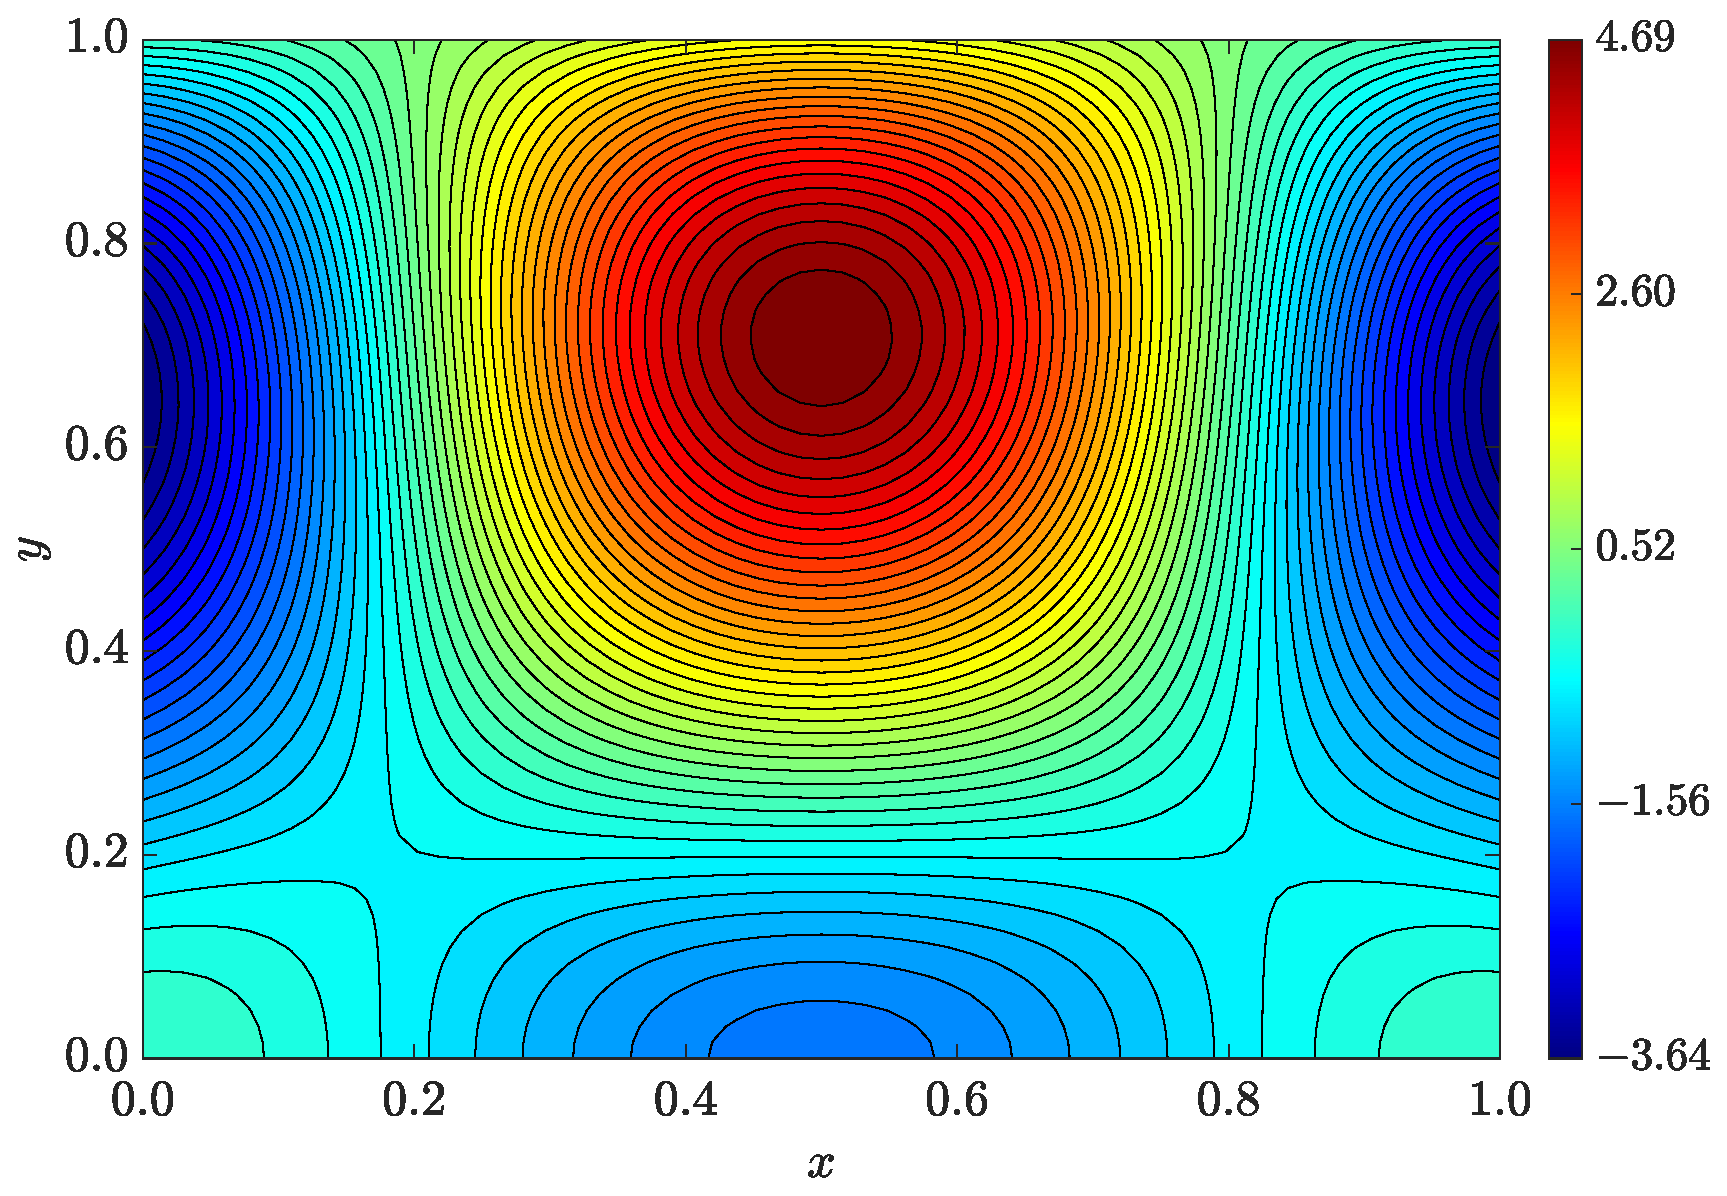
\includegraphics[width=\textwidth]{Figures/Exact_Map_NormErr_2nd_Betann_0.1_Re_1_Wi_1_epsilon_0_xi_0_alphaG_0_Dt_1e-06_at_0.05_tipsim_1_MMS_12_Wz.eps}
        \captionof{subfigure}{$\widetilde{\omega_{z}}$}
        \label{fig_solexawzCase11}
    \end{minipage}
    \hfill
    \begin{minipage}{0.48\textwidth}
        \centering
        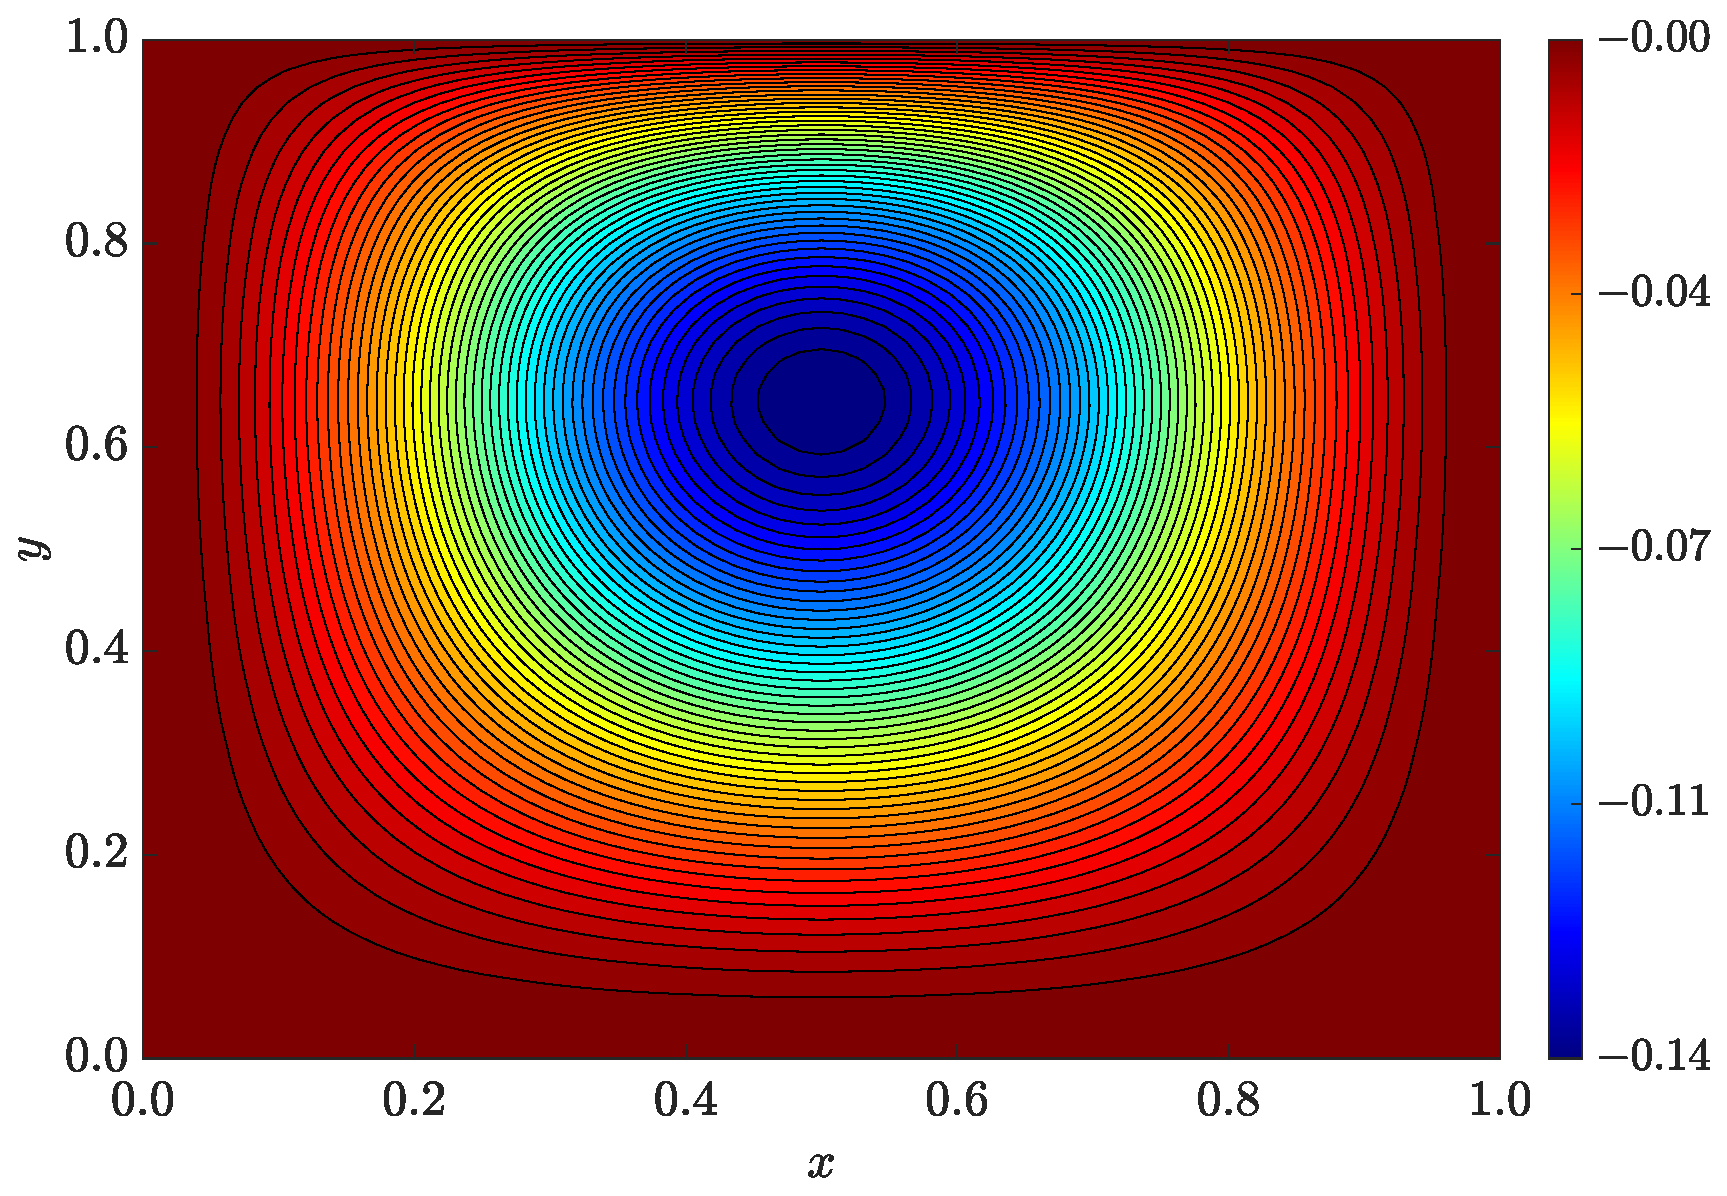
\includegraphics[width=\textwidth]{Figures/Exact_Map_NormErr_2nd_Betann_0.1_Re_1_Wi_1_epsilon_0_xi_0_alphaG_0_Dt_1e-06_at_0.05_tipsim_1_MMS_12_Psi.eps}
        \captionof{subfigure}{$\widetilde{\psi}$}
        \label{fig_solexapsiCase11}
    \end{minipage}
\end{frame}

%%%%%%%%%%%%%%%%%%%%%%%%%%%%%%%%%%%%%%%%%%%%%%%%%%%%%%%%%%%%%%
\begin{frame}{Soluções Manufaturadas}
    \centering
    \captionsetup{justification=centering}
    \captionof{figure}{Soluções manufaturadas no regime de estado estacionário para os tensores, considerando $\beta_{nn}=0.1$ e $a = 0.05$}
    \label{fig:sol_manufaturadas_31}
    \begin{minipage}{0.31\textwidth}
        \centering
        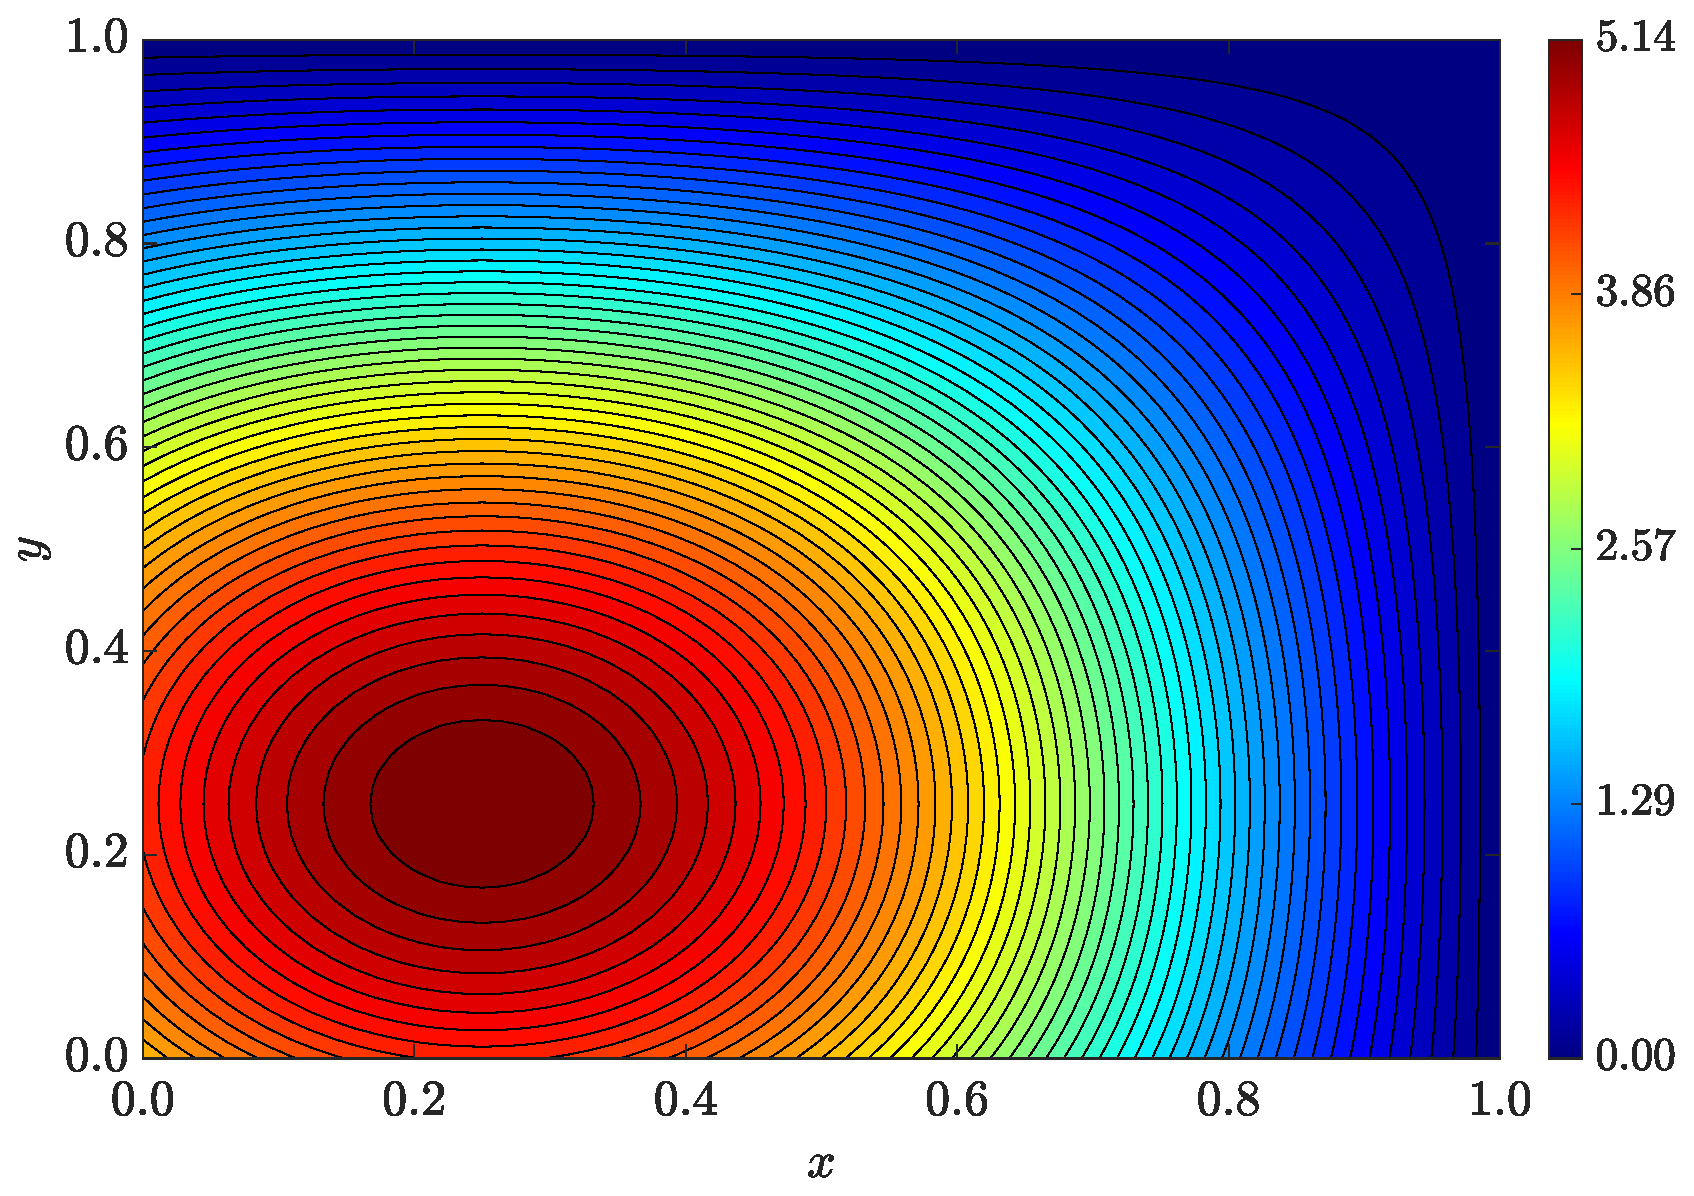
\includegraphics[width=\textwidth]{Figures/Exact_Map_NormErr_2nd_Betann_0.1_Re_1_Wi_1_epsilon_0_xi_0_alphaG_0_Dt_1e-06_at_0.05_tipsim_1_MMS_12_Txx.eps}
        \captionof{subfigure}{$\overline{T}_{xx}$}
        \label{fig_solexaTxxCase11}
    \end{minipage}
    \hfill
    \begin{minipage}{0.31\textwidth}
        \centering
        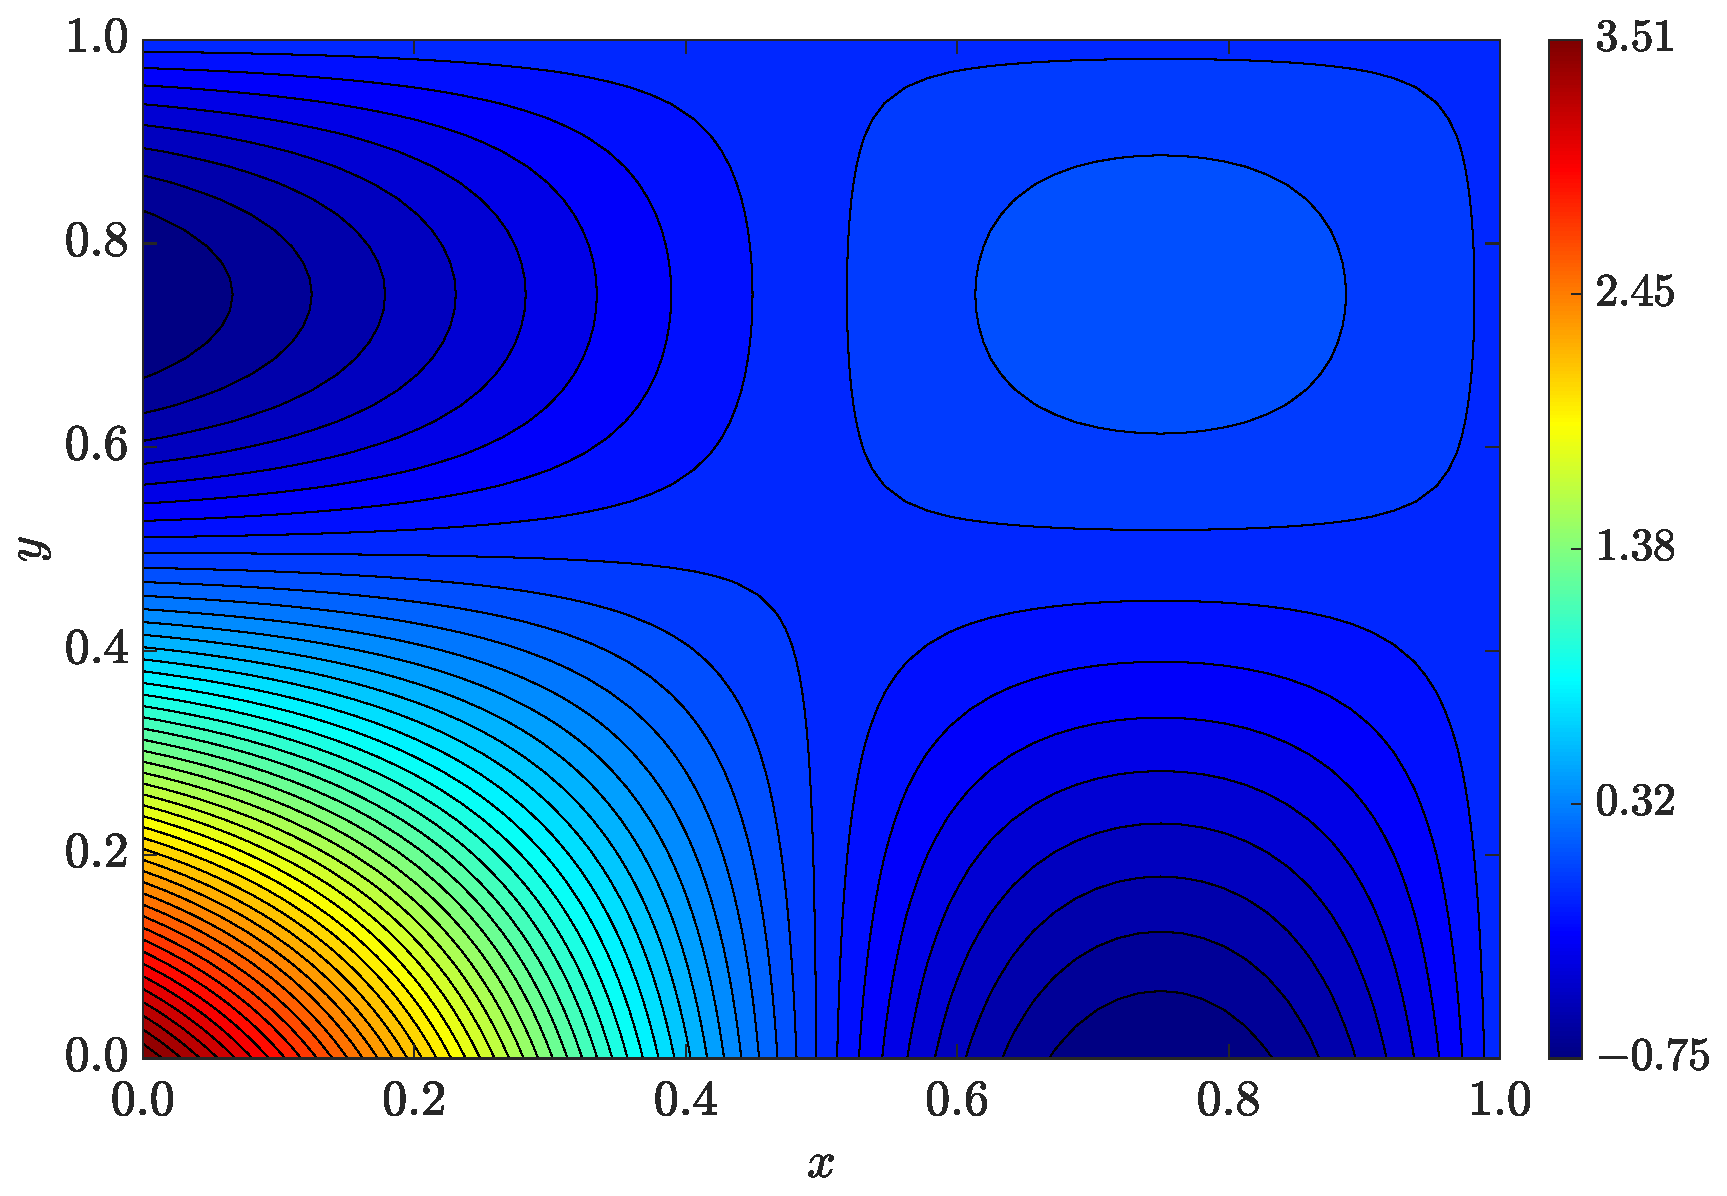
\includegraphics[width=\textwidth]{Figures/Exact_Map_NormErr_2nd_Betann_0.1_Re_1_Wi_1_epsilon_0_xi_0_alphaG_0_Dt_1e-06_at_0.05_tipsim_1_MMS_12_Txy.eps}
        \captionof{subfigure}{$\overline{T}_{xy}$}
        \label{fig_solexaTxyCase11}
    \end{minipage}
    \hfill
    \begin{minipage}{0.31\textwidth}
        \centering
        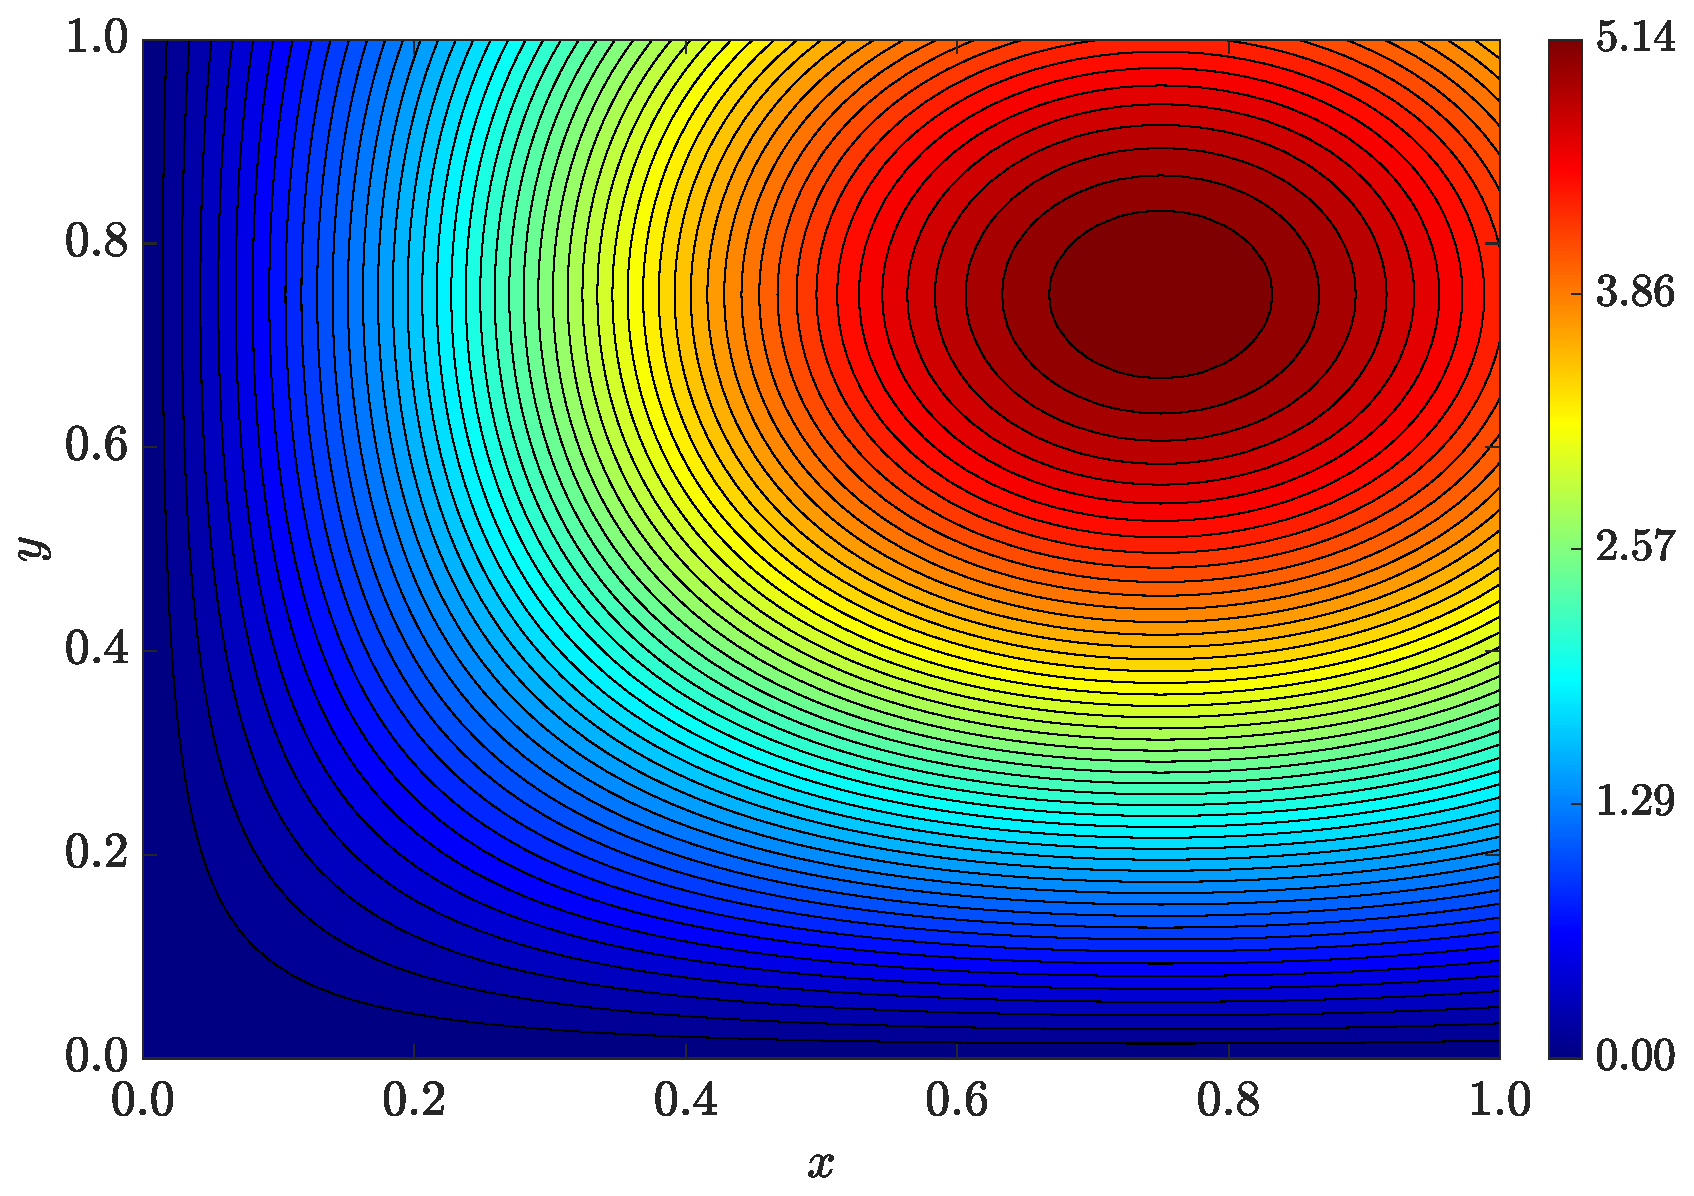
\includegraphics[width=\textwidth]{Figures/Exact_Map_NormErr_2nd_Betann_0.1_Re_1_Wi_1_epsilon_0_xi_0_alphaG_0_Dt_1e-06_at_0.05_tipsim_1_MMS_12_Tyy.eps}
        \captionof{subfigure}{$\overline{T}_{yy}$}
        \label{fig_solexaTyyCase11}
    \end{minipage}
\end{frame}

%%%%%%%%%%%%%%%%%%%%%%%%%%%%%%%%%%%%%%%%%%%%%%%%%%%%%%%%%%%%%%
\begin{frame}{Soluções Manufaturadas}
    \centering
    \captionsetup{justification=centering}
    \captionof{figure}{Soluções manufaturadas no regime de estado estacionário para os tensores, considerando $\beta_{nn}=0.1$ e $a = 0.05$}
    \label{fig:sol_manufaturadas_311}
    \begin{minipage}{0.31\textwidth}
        \centering
        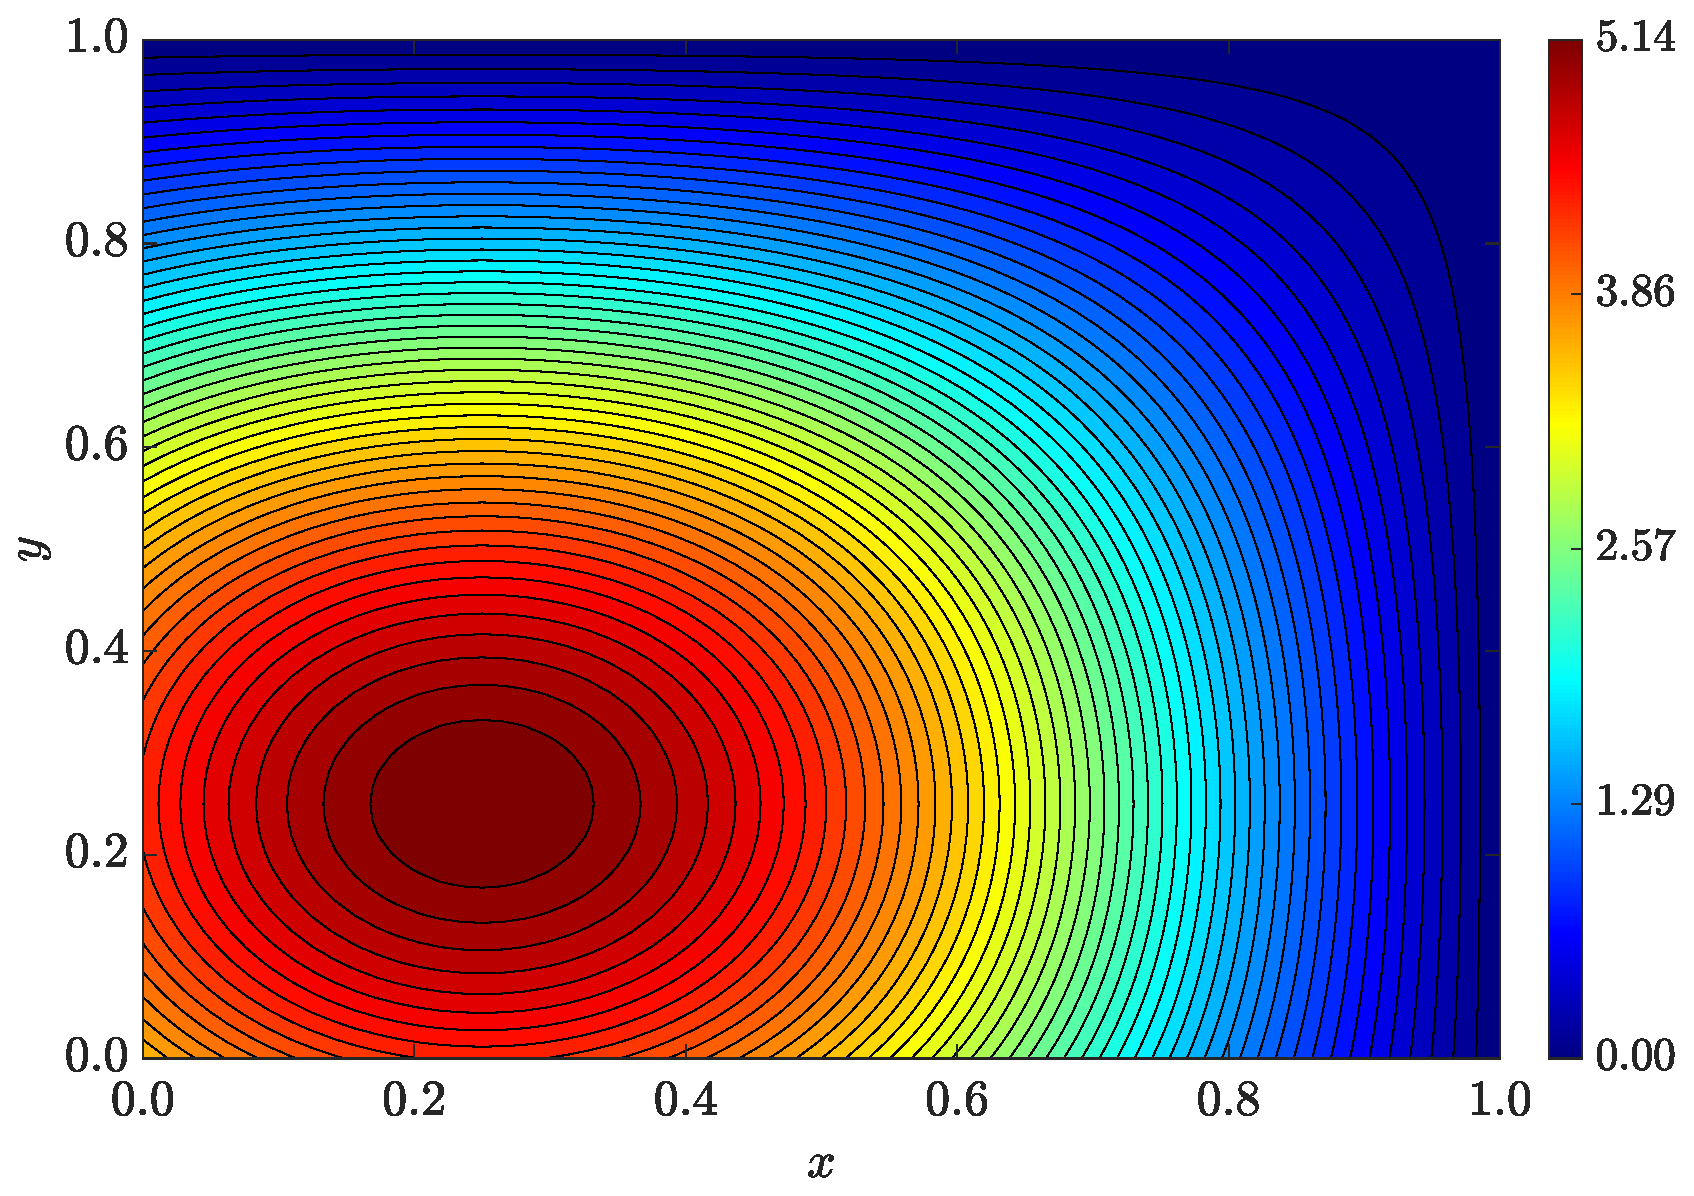
\includegraphics[width=\textwidth]{Figures/Exact_Map_NormErr_2nd_Betann_0.1_Re_1_Wi_1_epsilon_0_xi_0_alphaG_0_Dt_1e-06_at_0.05_tipsim_1_MMS_12_Txx.eps}
        \captionof{subfigure}{$\overline{T}_{xx}$}
        \label{fig_solexaTxxCase111}
    \end{minipage}
    \hfill
    \begin{minipage}{0.31\textwidth}
        \centering
        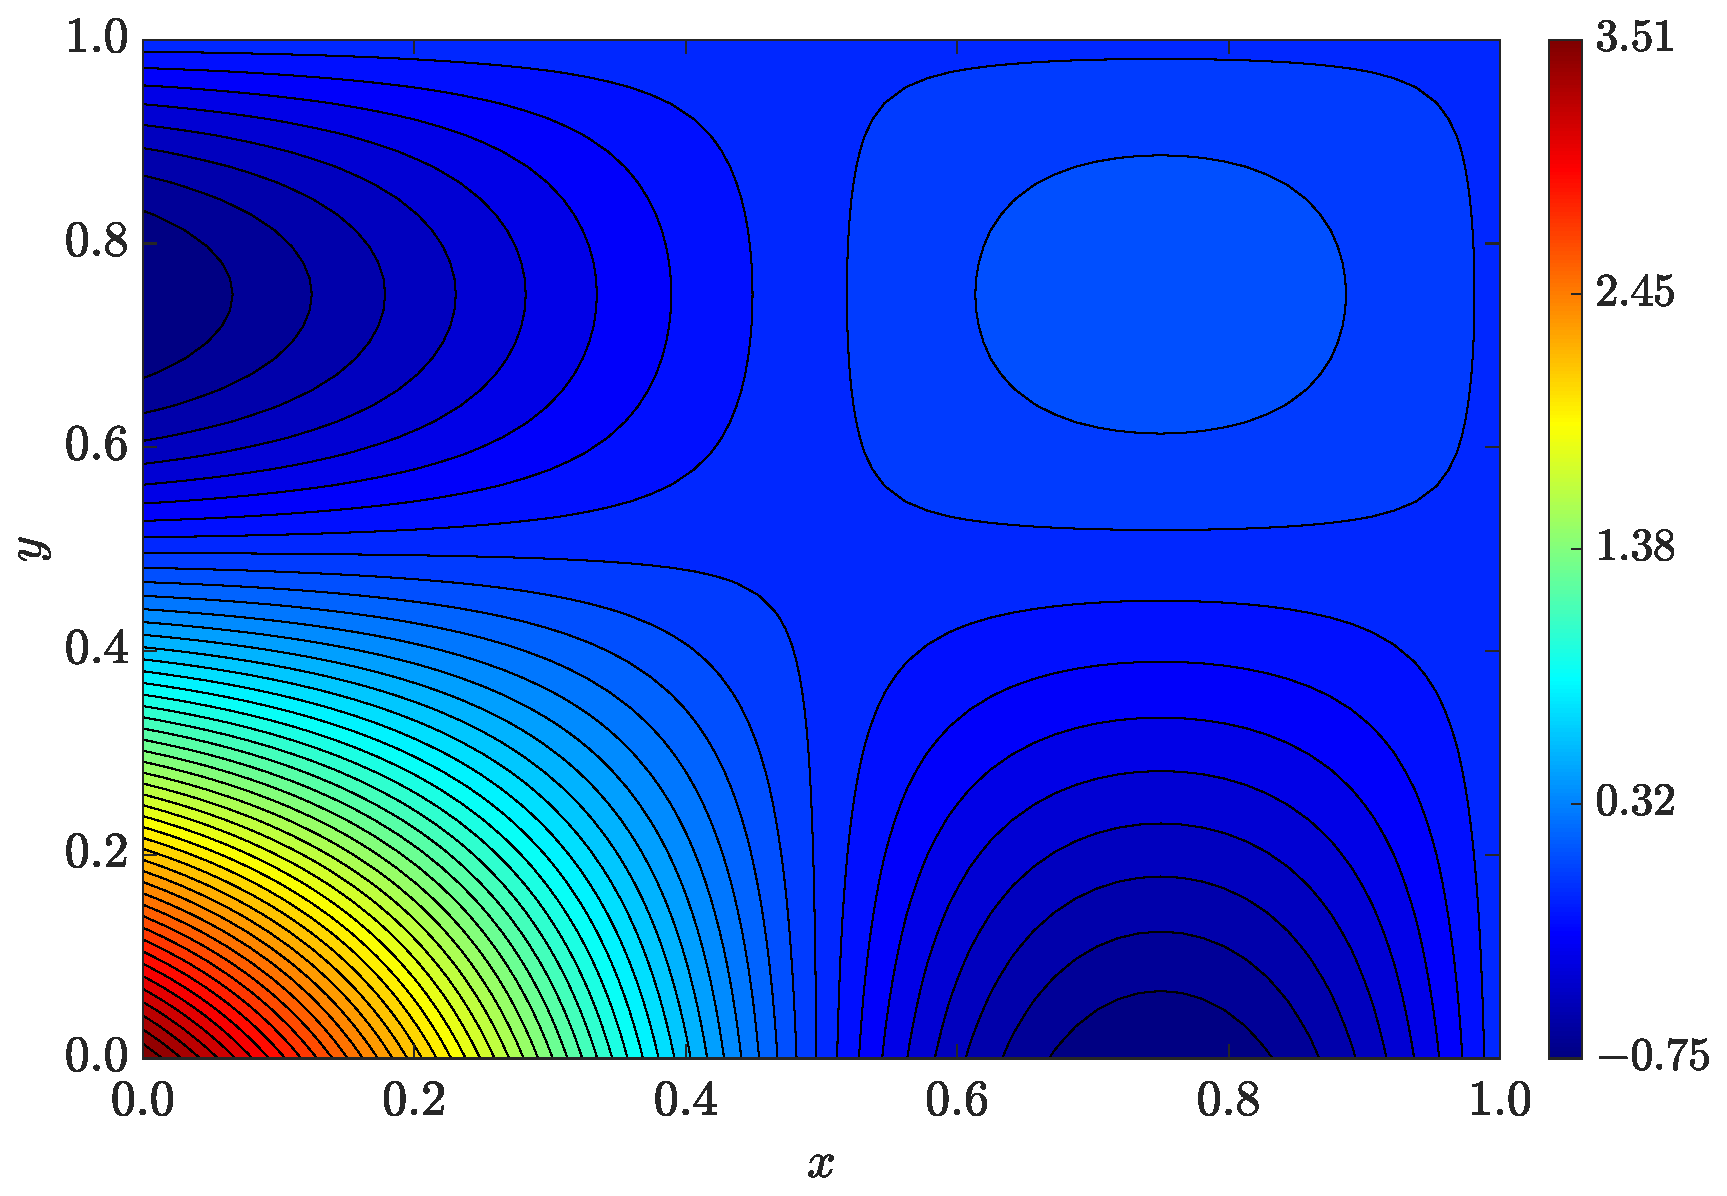
\includegraphics[width=\textwidth]{Figures/Exact_Map_NormErr_2nd_Betann_0.1_Re_1_Wi_1_epsilon_0_xi_0_alphaG_0_Dt_1e-06_at_0.05_tipsim_1_MMS_12_Txy.eps}
        \captionof{subfigure}{$\overline{T}_{xy}$}
        \label{fig_solexaTxyCase111}
    \end{minipage}
    \hfill
    \begin{minipage}{0.31\textwidth}
        \centering
        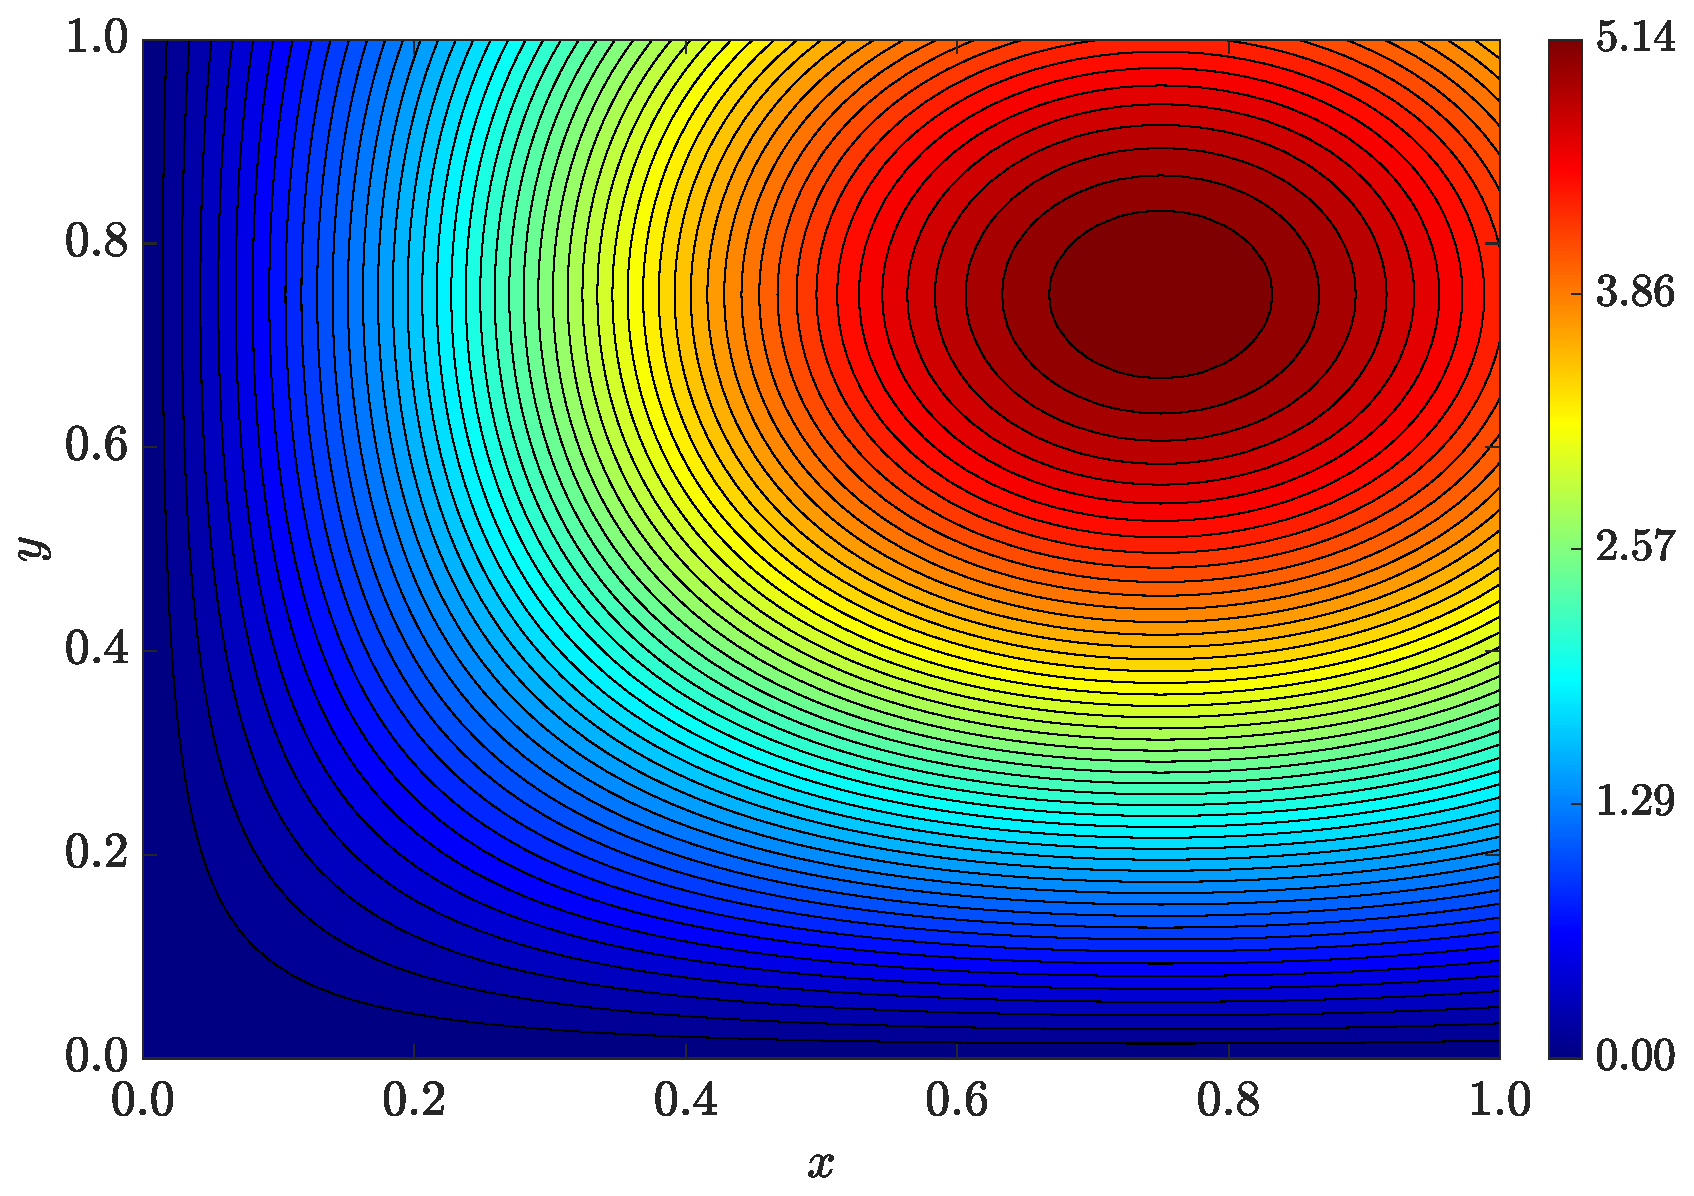
\includegraphics[width=\textwidth]{Figures/Exact_Map_NormErr_2nd_Betann_0.1_Re_1_Wi_1_epsilon_0_xi_0_alphaG_0_Dt_1e-06_at_0.05_tipsim_1_MMS_12_Tyy.eps}
        \captionof{subfigure}{$\overline{T}_{yy}$}
        \label{fig_solexaTyyCase111}
    \end{minipage}
\end{frame}

%%%%%%%%%%%%%%%%%%%%%%%%%%%%%%%%%%%%%%%%%%%%%%%%%%%%%%%%%%%%%%
\begin{frame}{Caso de verificação usando o modelo UCM}
    \centering
    \begin{table}[H]
    \caption{Erros numéricos e cálculo da ordem de convergência para a vorticidade $(\omega_{z})$, utilizando o parâmetro $Wi=1$, para o escoamento de fluido viscoelástico UCM.\label{tab_UCMWzResumida_1}}
\scriptsize{
    \begin{minipage}{0.49\textwidth}
    \begin{tabular*}{\textwidth}{@{\extracolsep\fill}cccc@{}}
    \hline
    \multirow{2}{*}{$\operatorname{Re}$} & \multirow{2}{*}{Malha} & \multicolumn{2}{c}{$\beta_{nn}=0.0$}\\ %\cline{2-10}
     & & Erro & Ordem \\
    \hline
    \multirow{7}{*}{1.00} & $17\times 17$ & 3.10e-03 & --- \\
    & $33\times 33$ & 2.93e-04 & 3.40 \\
    & $49\times 49$ & 6.78e-05 & 3.61 \\
    & $65\times 65$ & 2.31e-05 & 3.74 \\
    & $81\times 81$ & 9.80e-06 & 3.85 \\
    & $97\times 97$ & 4.72e-06 & 4.01 \\
    & $113\times 113$ & 2.46e-06 & 4.22 \\
    & $129\times 129$ & 1.41e-06 & 4.16 \\
    \hline
    \multirow{7}{*}{100.00} & $17\times 17$ & 3.10e-03 & --- \\
    & $33\times 33$ & 2.93e-04 & 3.40 \\
    & $49\times 49$ & 6.78e-05 & 3.61 \\
    & $65\times 65$ & 2.32e-05 & 3.74 \\
    & $81\times 81$ & 9.83e-06 & 3.84 \\
    & $97\times 97$ & 4.74e-06 & 4.00 \\
    & $113\times 113$ & 2.48e-06 & 4.21 \\
    & $129\times 129$ & 1.42e-06 & 4.16 \\
    \hline
    \end{tabular*}
    \end{minipage}
    \hfill
    \begin{minipage}{0.49\textwidth}
    \begin{tabular*}{\textwidth}{@{\extracolsep\fill}cccc@{}}
    \hline
    \multirow{2}{*}{$\operatorname{Re}$} & \multirow{2}{*}{Malha} & \multicolumn{2}{c}{$\beta_{nn}=0.0$}\\
     & & Erro & Ordem \\
    \hline
    \multirow{7}{*}{400.00} & $17\times 17$ & 3.10e-03 & --- \\
    & $33\times 33$ & 2.93e-04 & 3.40 \\
    & $49\times 49$ & 6.78e-05 & 3.61 \\
    & $65\times 65$ & 2.32e-05 & 3.74 \\
    & $81\times 81$ & 9.83e-06 & 3.84 \\
    & $97\times 97$ & 4.74e-06 & 4.00 \\
    & $113\times 113$ & 2.48e-06 & 4.21 \\
    & $129\times 129$ & 1.42e-06 & 4.16 \\
    \hline
    \multirow{7}{*}{1000.00} & $17\times 17$ & 3.10e-03 & --- \\
    & $33\times 33$ & 2.93e-04 & 3.40 \\
    & $49\times 49$ & 6.78e-05 & 3.61 \\
    & $65\times 65$ & 2.32e-05 & 3.74 \\
    & $81\times 81$ & 9.83e-06 & 3.84 \\
    & $97\times 97$ & 4.74e-06 & 4.00 \\
    & $113\times 113$ & 2.48e-06 & 4.21 \\
    & $129\times 129$ & 1.42e-06 & 4.16 \\
    \hline
    \end{tabular*}
    \end{minipage}
}
\end{table}
\end{frame}

%%%%%%%%%%%%%%%%%%%%%%%%%%%%%%%%%%%%%%%%%%%%%%%%%%%%%%%%%%%%%%
\begin{frame}{Caso de verificação usando o modelo UCM}
    \centering
    \captionsetup{justification=centering}
    \captionof{figure}{Erro para o campo de velocidades $(\overline{u},\tilde{v})$ utilizando $Re=100$, $\beta_{nn} = 0$ e $Wi=1$ para o escoamento de fluido viscoelástico como o modelo UCM}
    \label{fig:ucm_1}
    \begin{minipage}{0.49\textwidth}
        \centering
        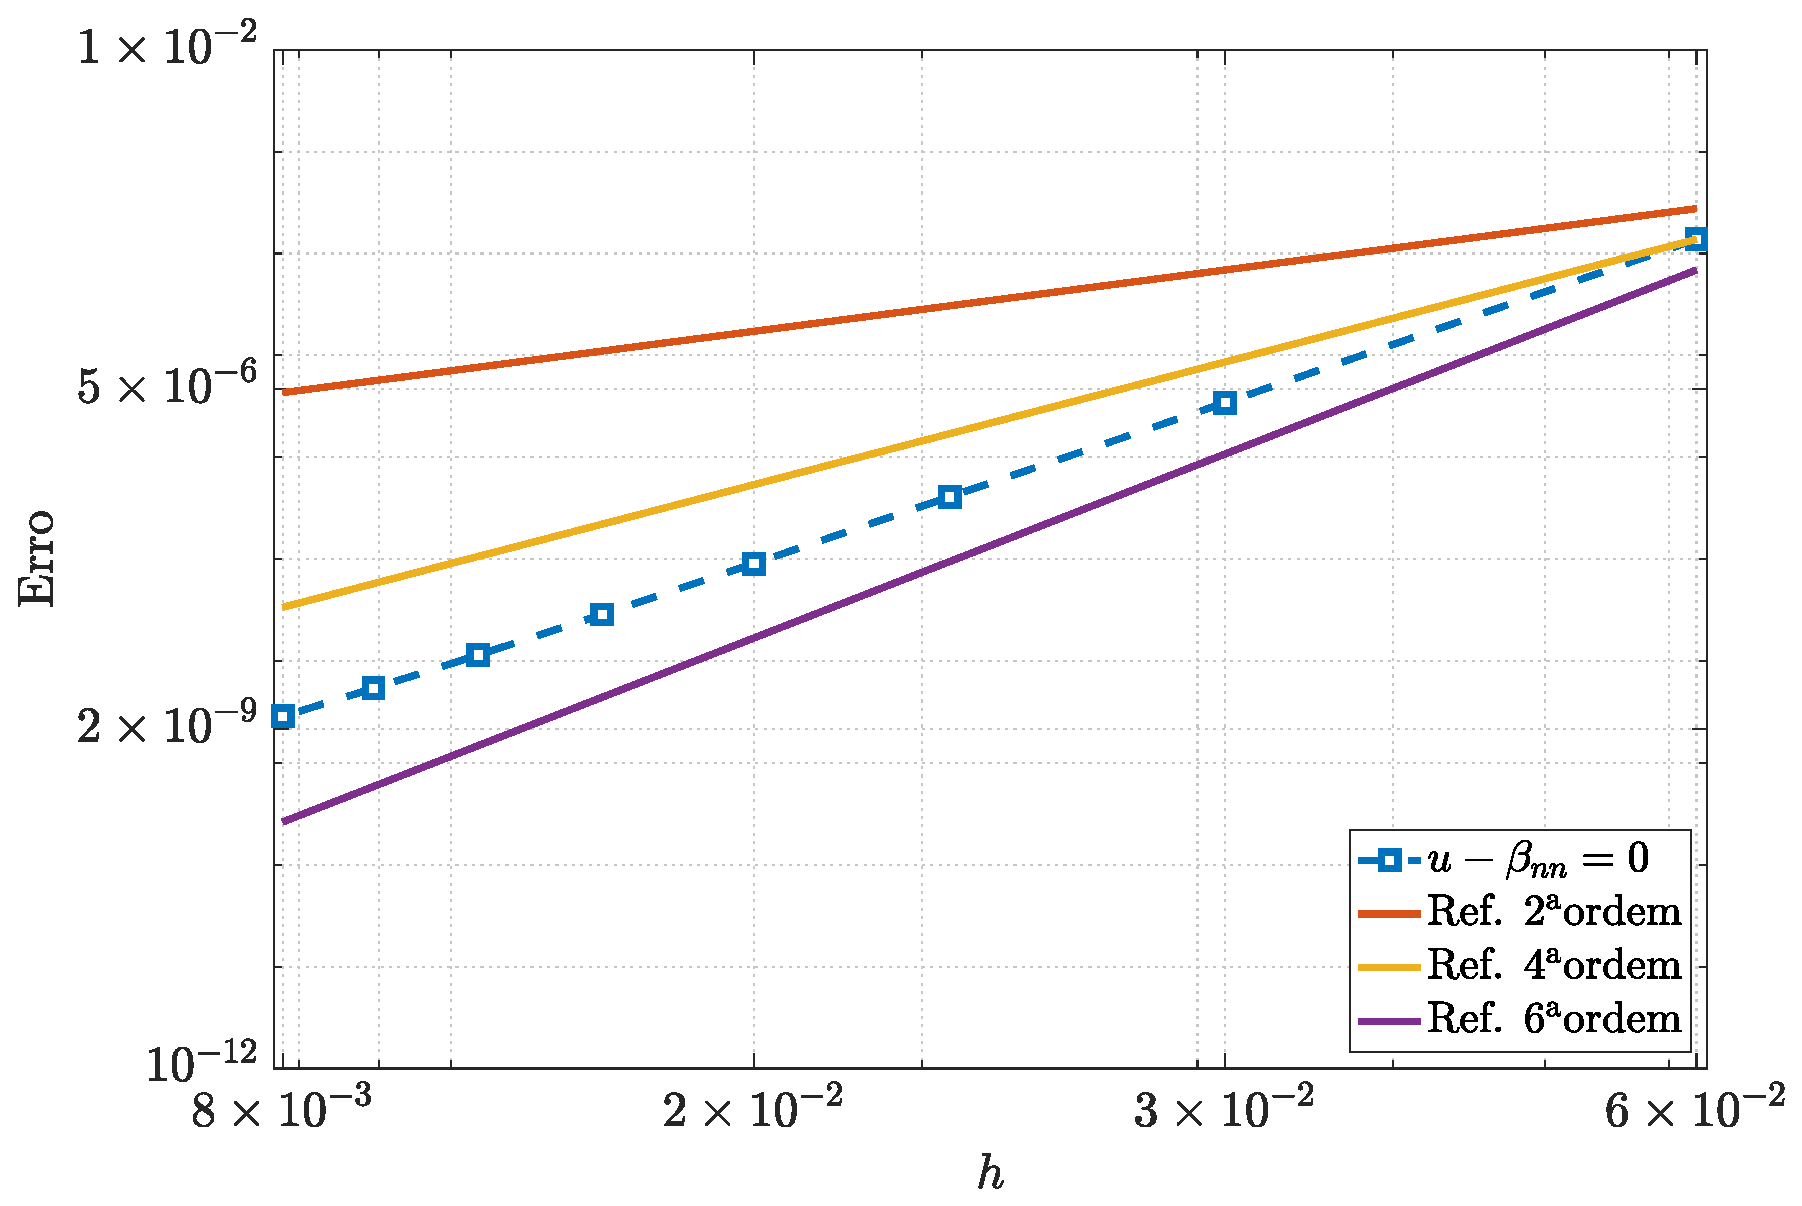
\includegraphics[width=\textwidth]{Figures/UCM/NormErr_2nd_Re_100_Wi_1_epsilon_0_xi_0_alphaG_0_Dt_1e-06_at_0.05_tipsim_1_MMS_12_U.eps}
        \captionof{subfigure}{$\overline{u}$}
        \label{ucm_u_Case11}
    \end{minipage}
    \hfill
    \begin{minipage}{0.49\textwidth}
        \centering
        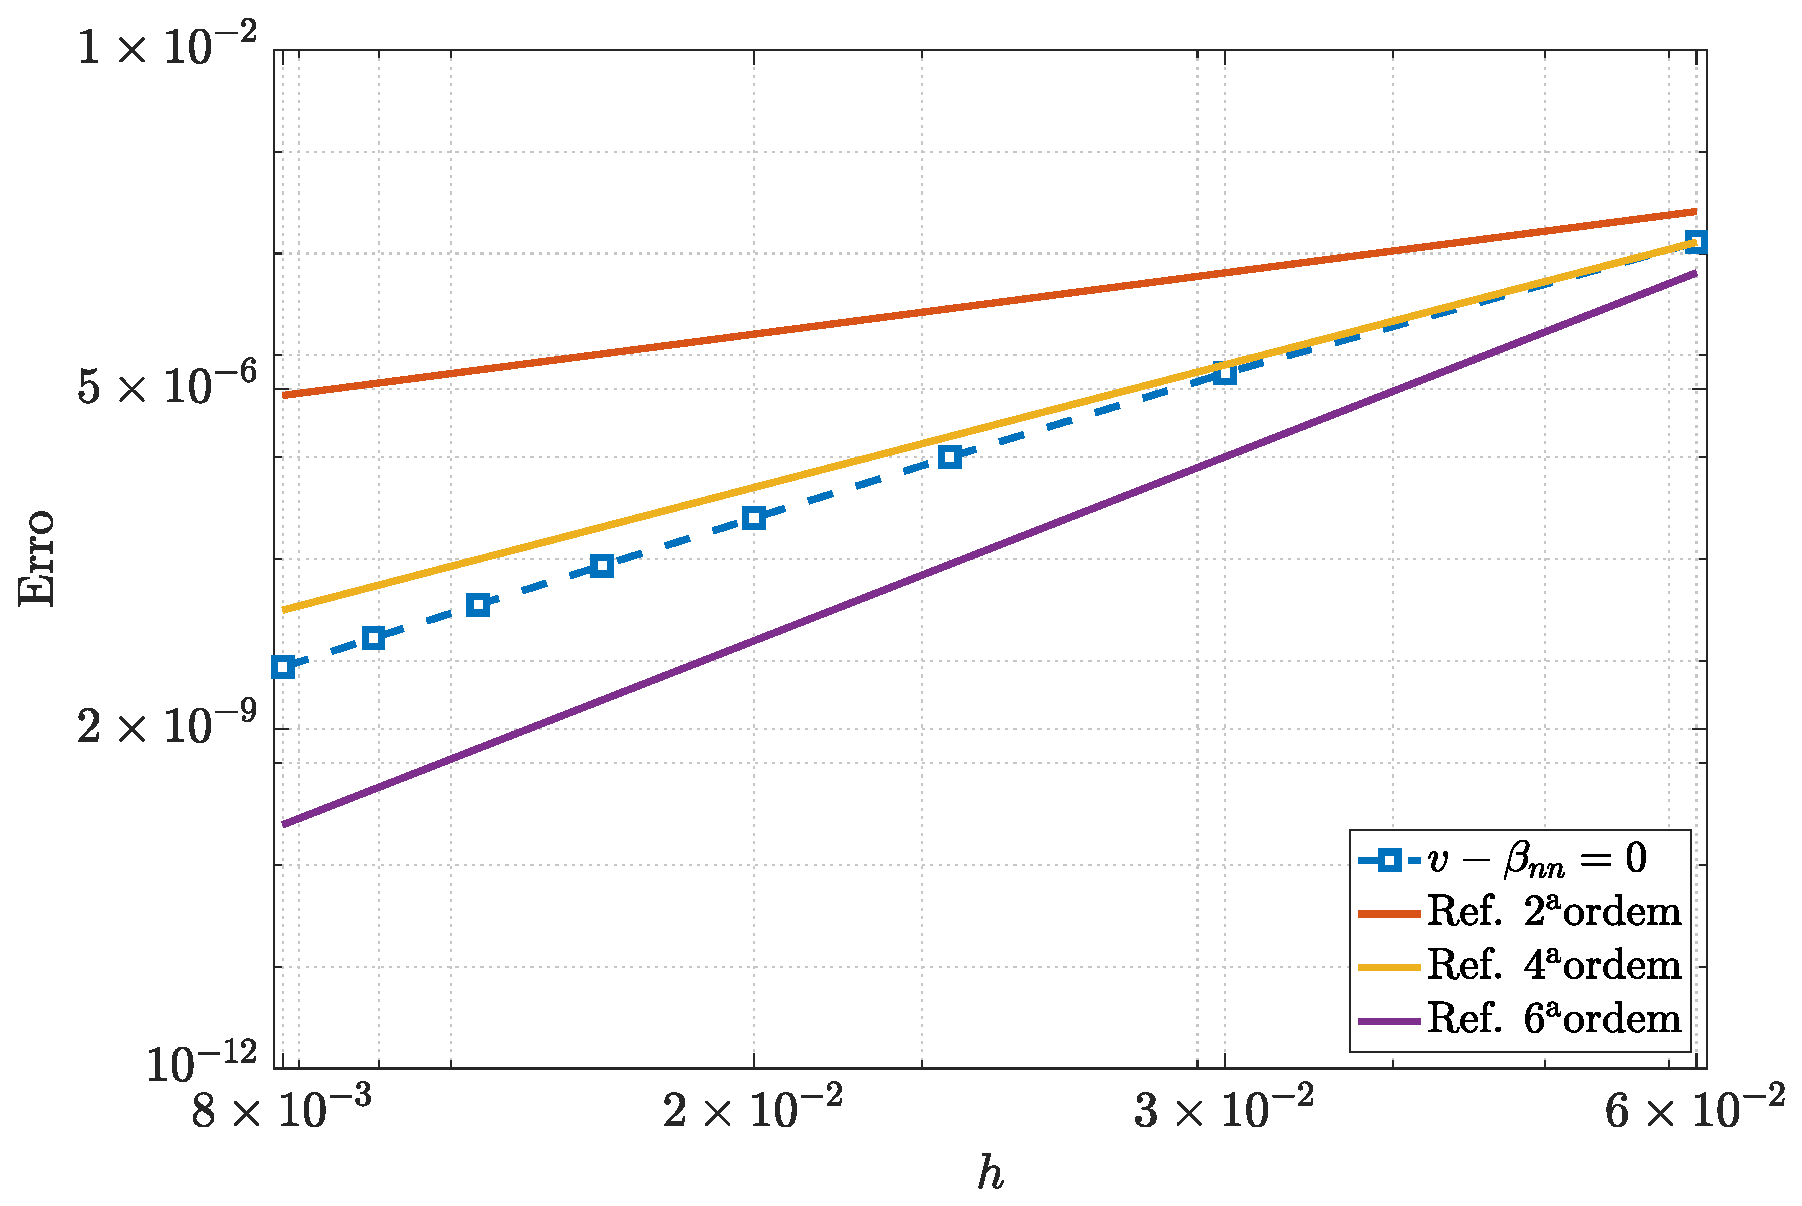
\includegraphics[width=\textwidth]{Figures/UCM/NormErr_2nd_Re_100_Wi_1_epsilon_0_xi_0_alphaG_0_Dt_1e-06_at_0.05_tipsim_1_MMS_12_V.eps}
        \captionof{subfigure}{$\tilde{v}$}
        \label{ucm_v_Case11}
    \end{minipage}
\end{frame}

%%%%%%%%%%%%%%%%%%%%%%%%%%%%%%%%%%%%%%%%%%%%%%%%%%%%%%%%%%%%%%
\begin{frame}{Caso de verificação usando o modelo UCM}
    \centering
    \captionsetup{justification=centering}
    \captionof{figure}{Erro para a vorticidade $(\tilde{\omega_{z}})$ e função de corrente $(\tilde{\psi})$, utilizando $Re=100$, $\beta_{nn} = 0$ e $Wi=1$ para o escoamento de fluido viscoelástico como o modelo UCM}
    \label{fig:ucm_2}
    \begin{minipage}{0.49\textwidth}
        \centering
        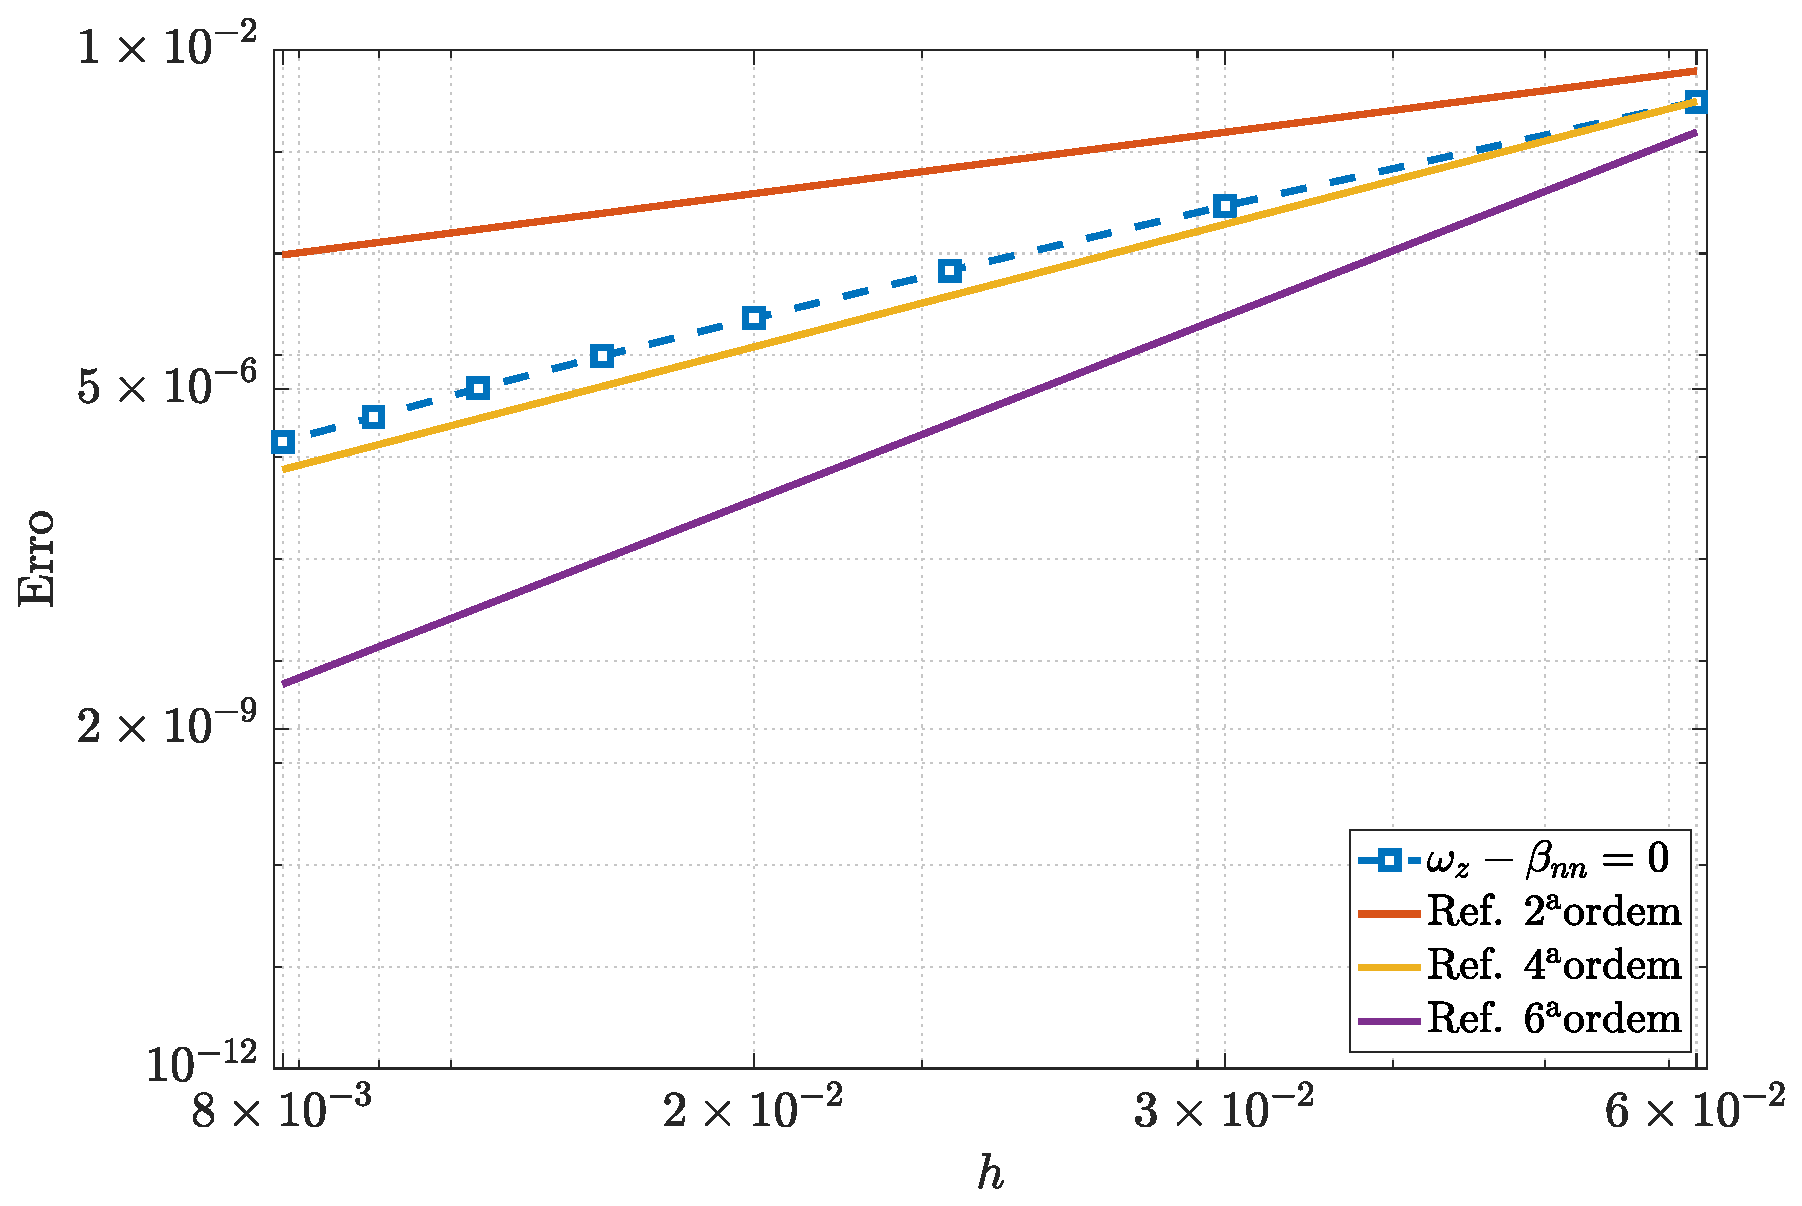
\includegraphics[width=\textwidth]{Figures/UCM/NormErr_2nd_Re_100_Wi_1_epsilon_0_xi_0_alphaG_0_Dt_1e-06_at_0.05_tipsim_1_MMS_12_Wz.eps}
        \captionof{subfigure}{$\tilde{\omega_{z}}$}
        \label{ucm_wz_Case11}
    \end{minipage}
    \hfill
    \begin{minipage}{0.49\textwidth}
        \centering
        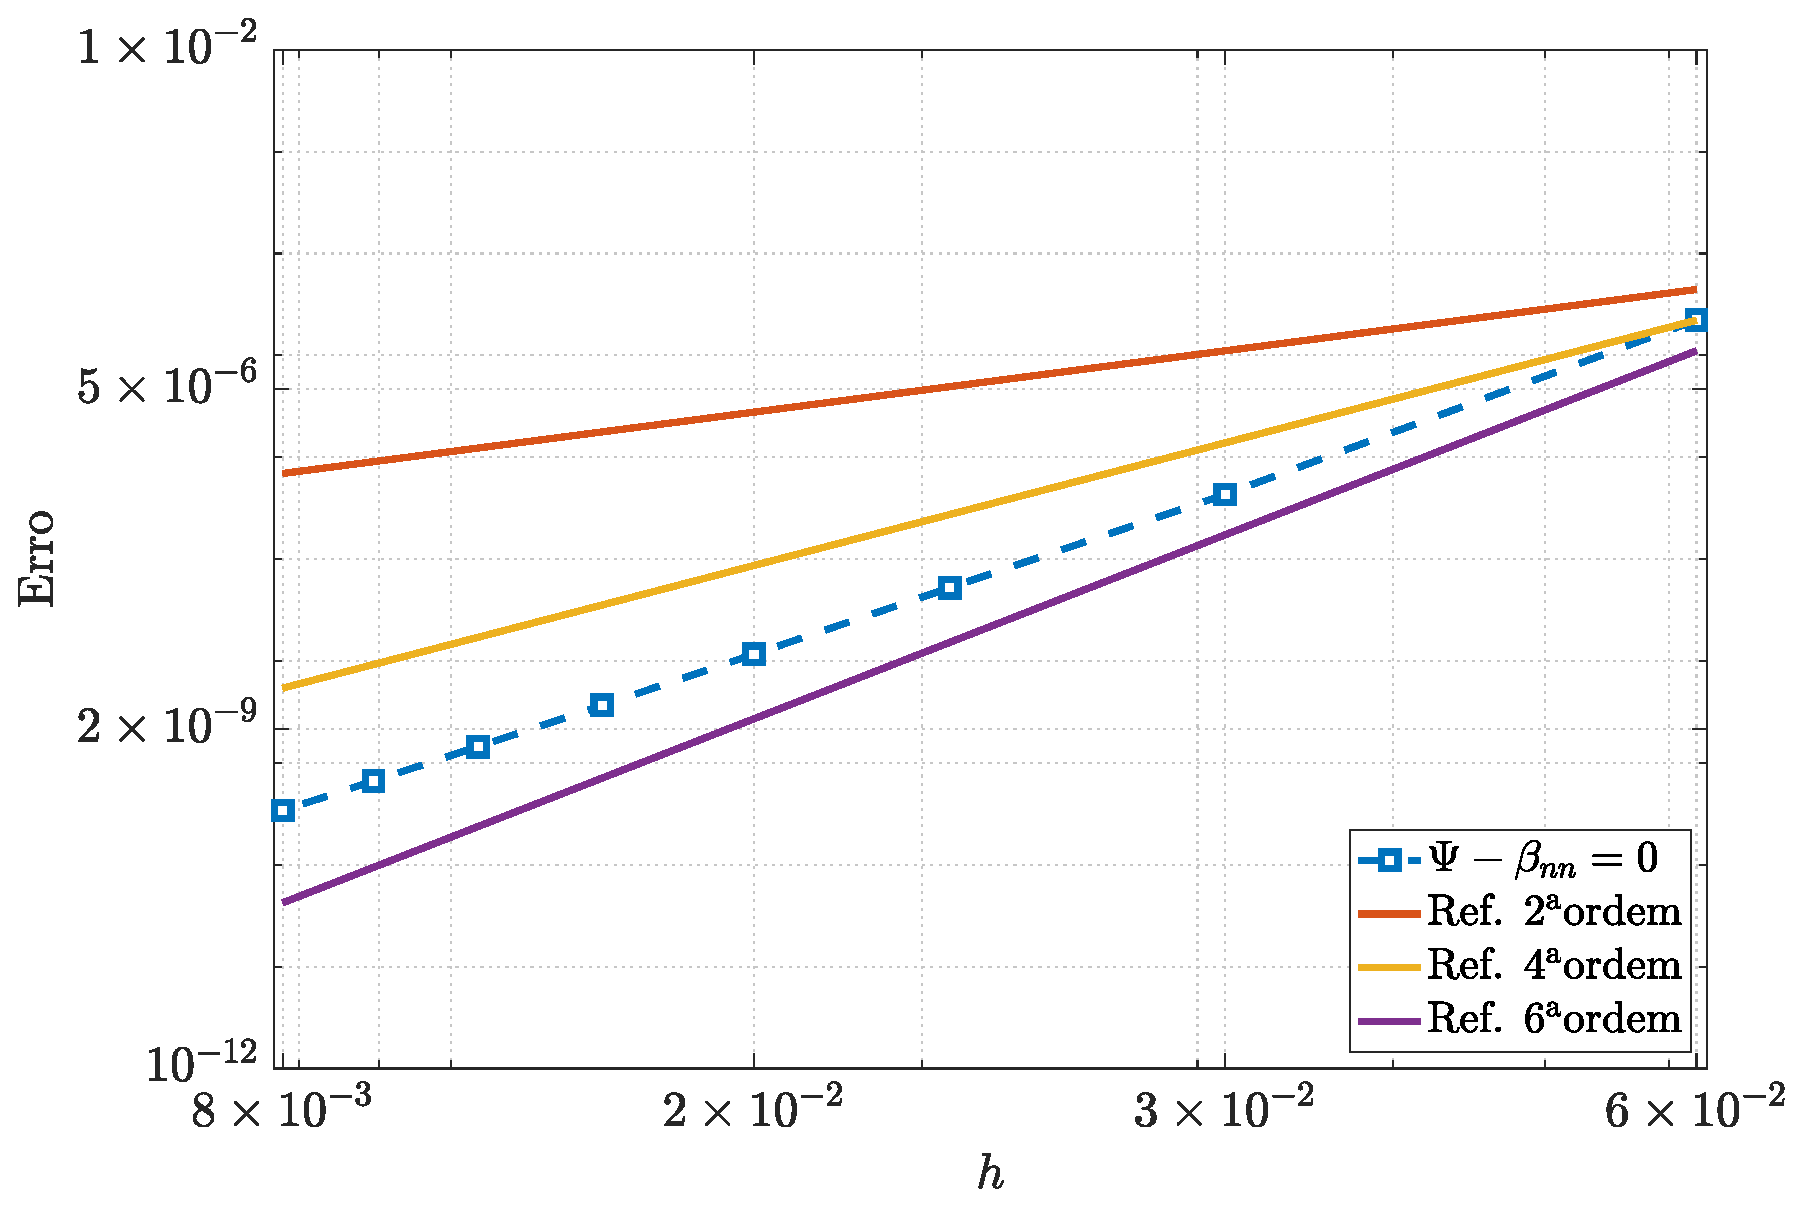
\includegraphics[width=\textwidth]{Figures/UCM/NormErr_2nd_Re_100_Wi_1_epsilon_0_xi_0_alphaG_0_Dt_1e-06_at_0.05_tipsim_1_MMS_12_Psi.eps}
        \captionof{subfigure}{$\tilde{\psi}$}
        \label{ucm_psi_Case11}
    \end{minipage}
\end{frame}

%%%%%%%%%%%%%%%%%%%%%%%%%%%%%%%%%%%%%%%%%%%%%%%%%%%%%%%%%%%%%%
\begin{frame}{Caso de verificação usando o modelo UCM}
    \centering
    \captionsetup{justification=centering}
    \captionof{figure}{Erro para as componentes dos tensores de tensões, utilizando $Re=100$, $\beta_{nn} = 0$ e $Wi=1$ para o escoamento de fluido viscoelástico como o modelo UCM}
    \label{fig:ucm_3}
    \begin{minipage}{0.325\textwidth}
        \centering
        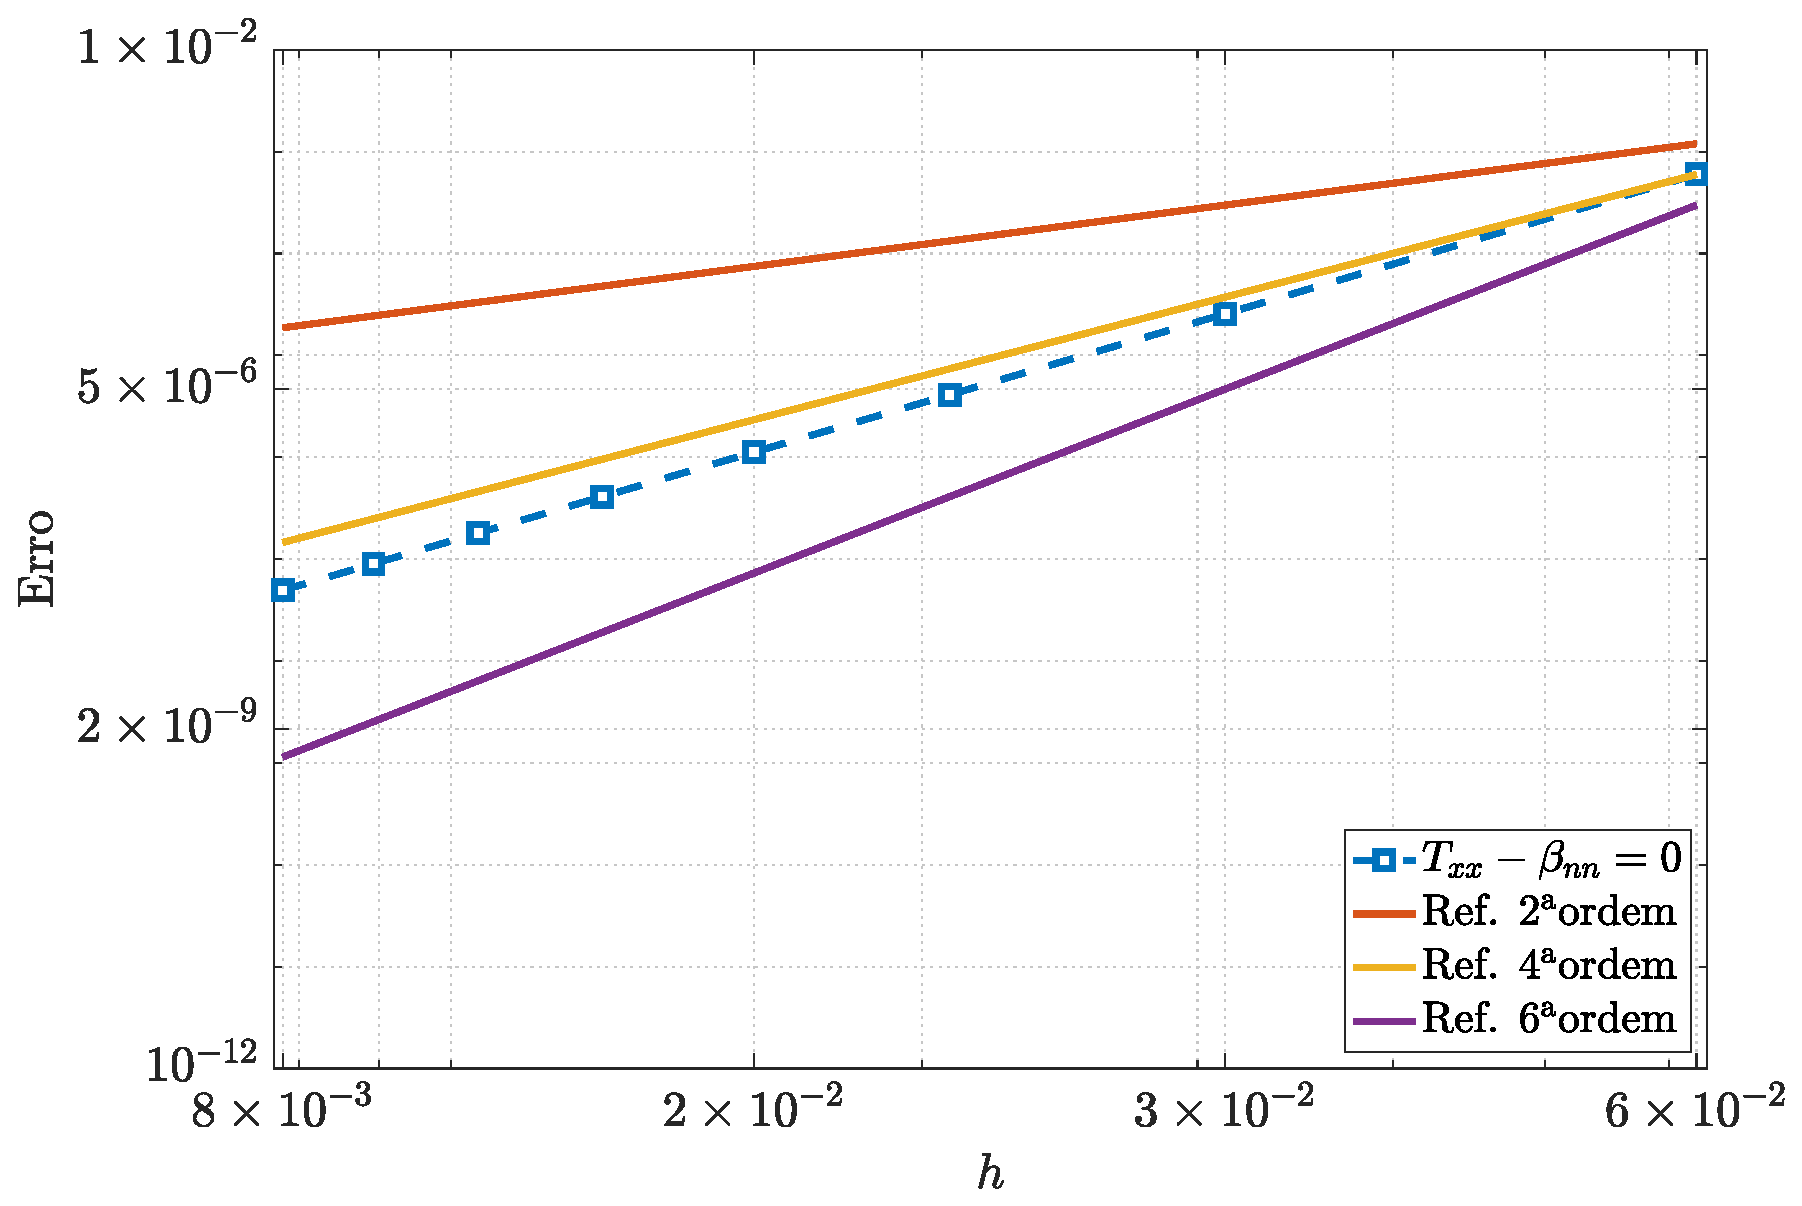
\includegraphics[width=\textwidth]{Figures/UCM/NormErr_2nd_Re_100_Wi_1_epsilon_0_xi_0_alphaG_0_Dt_1e-06_at_0.05_tipsim_1_MMS_12_Txx.eps}
        \captionof{subfigure}{$\overline{T_{xx}}$}
        \label{ucm_txx_Case11}
    \end{minipage}
    \hfill
    \begin{minipage}{0.325\textwidth}
        \centering
        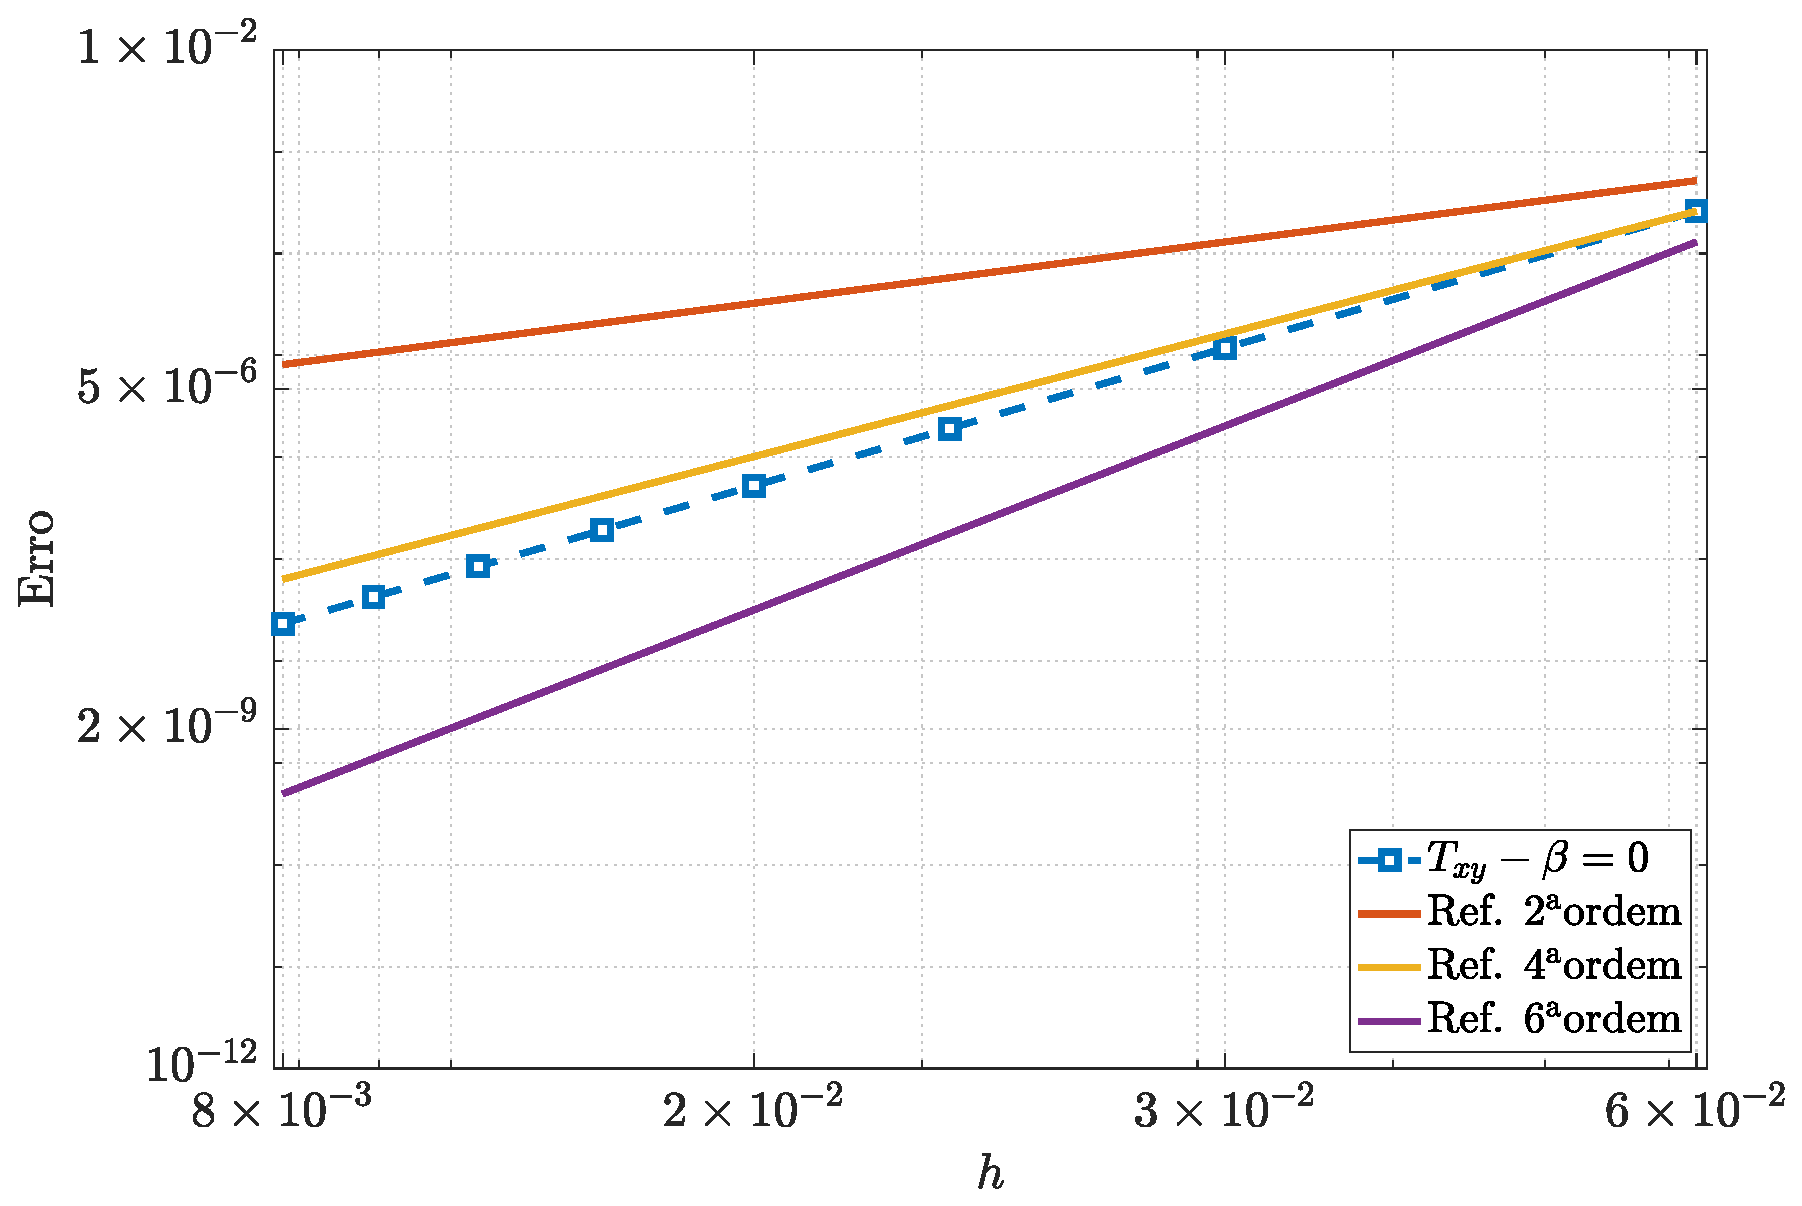
\includegraphics[width=\textwidth]{Figures/UCM/NormErr_2nd_Re_100_Wi_1_epsilon_0_xi_0_alphaG_0_Dt_1e-06_at_0.05_tipsim_1_MMS_12_Txy.eps}
        \captionof{subfigure}{$\overline{T_{xy}}$}
        \label{ucm_txy_Case11}
    \end{minipage}
    \hfill
    \begin{minipage}{0.325\textwidth}
        \centering
        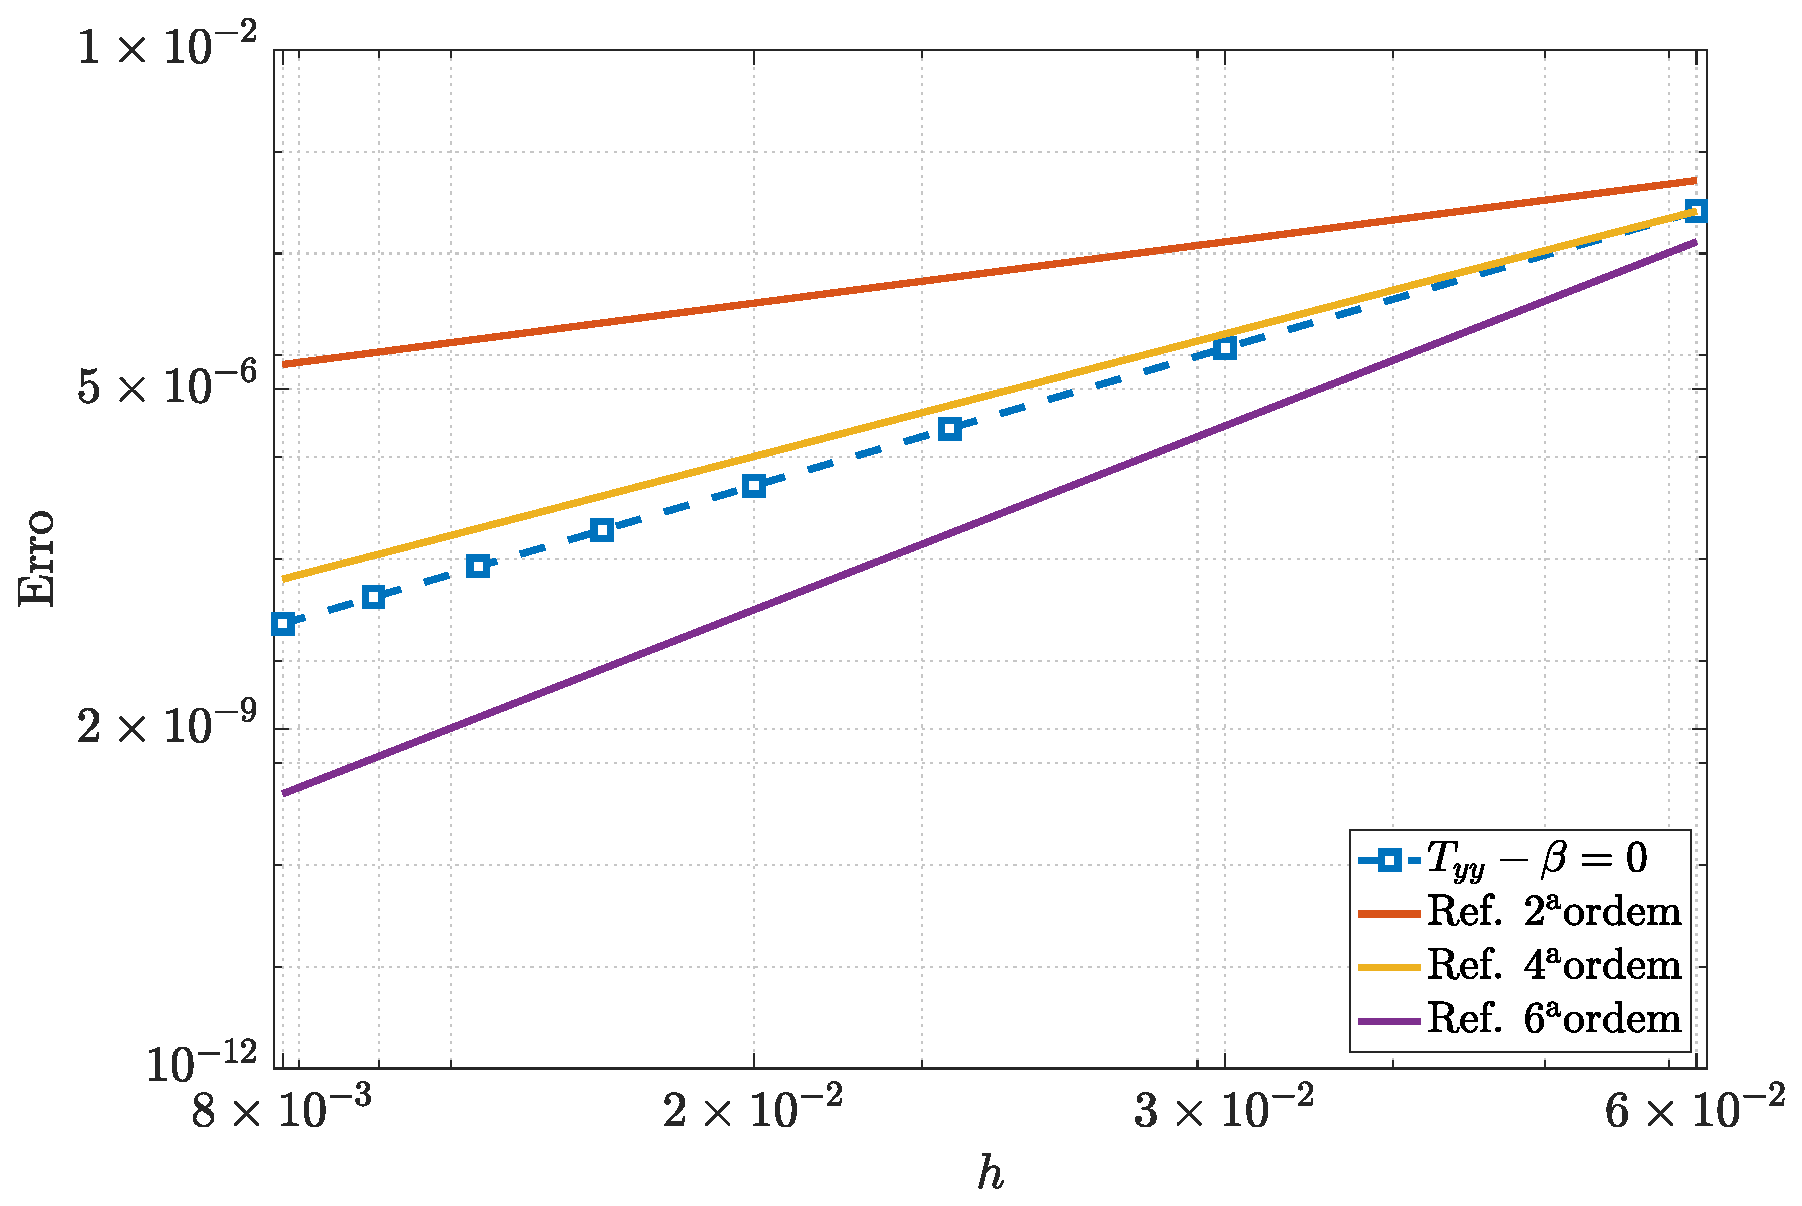
\includegraphics[width=\textwidth]{Figures/UCM/NormErr_2nd_Re_100_Wi_1_epsilon_0_xi_0_alphaG_0_Dt_1e-06_at_0.05_tipsim_1_MMS_12_Tyy.eps}
        \captionof{subfigure}{$\overline{T_{yy}}$}
        \label{ucm_tyy_Case11}
    \end{minipage}
\end{frame}

%%%%%%%%%%%%%%%%%%%%%%%%%%%%%%%%%%%%%%%%%%%%%%%%%%%%%%%%%%%%%%
\begin{frame}{Caso de verificação usando o modelo Oldroyd-B}
    \centering
    \begin{table}[H]
\caption{Erros numéricos e cálculo da ordem de convergência para a vorticidade $(\omega_{z})$, utilizando o parâmetro $Wi=1$, para o escoamento de fluido viscoelástico Oldroyd-B.\label{tab_OldroydBWzResumida}}
\scriptsize{
    \begin{tabular*}{\textwidth}{@{\extracolsep\fill}cccccccccc@{}}
    \hline
    \multirow{2}{*}{$\operatorname{Re}$} & \multirow{2}{*}{Malha} & \multicolumn{2}{c}{$\beta_{nn}=0.1$}  & \multicolumn{2}{c}{$\beta_{nn}=0.5$}  & \multicolumn{2}{c}{$\beta_{nn}=0.9$}  & \multicolumn{2}{c}{$\beta_{nn}=1.0$}\\ %\cline{2-10}
     & & Erro & Ordem & Erro & Ordem & Erro & Ordem & Erro & Ordem \\
    \hline
    \multirow{7}{*}{1.00} & $17\times 17$ & 2.23e-03 & --- & 2.08e-03 & --- & 1.96e-03 & --- & 1.93e-03 & --- \\
    & $33\times 33$ & 2.02e-04 & 3.47 & 1.51e-04 & 3.79 & 1.23e-04 & 4.00 & 1.18e-04 & 4.03 \\
    & $49\times 49$ & 4.26e-05 & 3.84 & 2.50e-05 & 4.44 & 1.92e-05 & 4.57 & 1.84e-05 & 4.58 \\
    & $65\times 65$ & 1.28e-05 & 4.17 & 6.43e-06 & 4.71 & 5.05e-06 & 4.65 & 4.85e-06 & 4.63 \\
    & $81\times 81$ & 4.68e-06 & 4.52 & 2.23e-06 & 4.74 & 1.79e-06 & 4.63 & 1.73e-06 & 4.61 \\
    & $97\times 97$ & 1.92e-06 & 4.90 & 9.34e-07 & 4.78 & 7.68e-07 & 4.65 & 7.45e-07 & 4.63 \\
    & $113\times 113$ & 8.58e-07 & 5.21 & 4.47e-07 & 4.77 & 3.80e-07 & 4.57 & 3.71e-07 & 4.52 \\
    & $129\times 129$ & 4.34e-07 & 5.10 & 2.59e-07 & 4.11 & 2.30e-07 & 3.76 & 2.26e-07 & 3.71 \\
    \hline\hline
    \multirow{7}{*}{100.00} & $17\times 17$ & 2.27e-03 & --- & 2.27e-03 & --- & 2.26e-03 & --- & 2.26e-03 & --- \\
    & $33\times 33$ & 2.20e-04 & 3.37 & 2.19e-04 & 3.37 & 2.18e-04 & 3.37 & 2.18e-04 & 3.37 \\
    & $49\times 49$ & 5.20e-05 & 3.56 & 5.15e-05 & 3.57 & 5.11e-05 & 3.58 & 5.10e-05 & 3.59 \\
    & $65\times 65$ & 1.82e-05 & 3.66 & 1.79e-05 & 3.68 & 1.76e-05 & 3.70 & 1.75e-05 & 3.71 \\
    & $81\times 81$ & 7.84e-06 & 3.76 & 7.65e-06 & 3.80 & 7.47e-06 & 3.84 & 7.43e-06 & 3.85 \\
    & $97\times 97$ & 3.83e-06 & 3.93 & 3.70e-06 & 3.99 & 3.57e-06 & 4.05 & 3.54e-06 & 4.06 \\
    & $113\times 113$ & 2.04e-06 & 4.10 & 1.94e-06 & 4.19 & 1.85e-06 & 4.27 & 1.83e-06 & 4.29 \\
    & $129\times 129$ & 1.21e-06 & 3.89 & 1.13e-06 & 4.02 & 1.07e-06 & 4.13 & 1.05e-06 & 4.16 \\
    \hline
    \end{tabular*}
}
\end{table}
\end{frame}

%%%%%%%%%%%%%%%%%%%%%%%%%%%%%%%%%%%%%%%%%%%%%%%%%%%%%%%%%%%%%%
\begin{frame}{Caso de verificação usando o modelo Oldroyd-B}
    \centering
    \begin{table}[H]
\caption{Erros numéricos e cálculo da ordem de convergência para a vorticidade $(\omega_{z})$, utilizando o parâmetro $Wi=1$, para o escoamento de fluido viscoelástico Oldroyd-B.\label{tab_OldroydBWzResumida_2}}
\scriptsize{
    \begin{tabular*}{\textwidth}{@{\extracolsep\fill}cccccccccc@{}}
    \hline
    \multirow{2}{*}{$\operatorname{Re}$} & \multirow{2}{*}{Malha} & \multicolumn{2}{c}{$\beta_{nn}=0.1$}  & \multicolumn{2}{c}{$\beta_{nn}=0.5$}  & \multicolumn{2}{c}{$\beta_{nn}=0.9$}  & \multicolumn{2}{c}{$\beta_{nn}=1.0$}\\ %\cline{2-10}
     & & Erro & Ordem & Erro & Ordem & Erro & Ordem & Erro & Ordem \\
    \hline
    \multirow{7}{*}{400.00} & $17\times 17$ & 2.27e-03 & --- & 2.27e-03 & --- & 2.27e-03 & --- & 2.27e-03 & --- \\
    & $33\times 33$ & 2.20e-04 & 3.37 & 2.20e-04 & 3.37 & 2.20e-04 & 3.37 & 2.20e-04 & 3.37 \\
    & $49\times 49$ & 5.21e-05 & 3.56 & 5.19e-05 & 3.56 & 5.18e-05 & 3.56 & 5.18e-05 & 3.56 \\
    & $65\times 65$ & 1.82e-05 & 3.65 & 1.81e-05 & 3.66 & 1.81e-05 & 3.66 & 1.81e-05 & 3.66 \\
    & $81\times 81$ & 7.88e-06 & 3.75 & 7.83e-06 & 3.76 & 7.79e-06 & 3.77 & 7.78e-06 & 3.77 \\
    & $97\times 97$ & 3.86e-06 & 3.92 & 3.83e-06 & 3.93 & 3.80e-06 & 3.94 & 3.79e-06 & 3.95 \\
    & $113\times 113$ & 2.05e-06 & 4.09 & 2.03e-06 & 4.11 & 2.01e-06 & 4.12 & 2.01e-06 & 4.13 \\
    & $129\times 129$ & 1.23e-06 & 3.86 & 1.21e-06 & 3.89 & 1.19e-06 & 3.92 & 1.19e-06 & 3.93 \\
    \hline\hline
    \multirow{7}{*}{1000.00} & $17\times 17$ & 2.27e-03 & --- & 2.27e-03 & --- & 2.27e-03 & --- & 2.27e-03 & --- \\
    & $33\times 33$ & 2.20e-04 & 3.37 & 2.20e-04 & 3.37 & 2.20e-04 & 3.37 & 2.20e-04 & 3.37 \\
    & $49\times 49$ & 5.21e-05 & 3.56 & 5.20e-05 & 3.56 & 5.20e-05 & 3.56 & 5.20e-05 & 3.56 \\
    & $65\times 65$ & 1.82e-05 & 3.65 & 1.82e-05 & 3.65 & 1.82e-05 & 3.65 & 1.82e-05 & 3.65 \\
    & $81\times 81$ & 7.89e-06 & 3.75 & 7.87e-06 & 3.76 & 7.86e-06 & 3.76 & 7.85e-06 & 3.76 \\
    & $97\times 97$ & 3.86e-06 & 3.92 & 3.85e-06 & 3.92 & 3.84e-06 & 3.92 & 3.84e-06 & 3.92 \\
    & $113\times 113$ & 2.06e-06 & 4.08 & 2.05e-06 & 4.09 & 2.04e-06 & 4.09 & 2.04e-06 & 4.09 \\
    & $129\times 129$ & 1.23e-06 & 3.86 & 1.22e-06 & 3.87 & 1.22e-06 & 3.87 & 1.22e-06 & 3.88 \\
    \hline
    \end{tabular*}
}
\end{table}
\end{frame}

%%%%%%%%%%%%%%%%%%%%%%%%%%%%%%%%%%%%%%%%%%%%%%%%%%%%%%%%%%%%%%
\begin{frame}{Caso de verificação usando o modelo Oldroyd-B}
    \centering
    \captionsetup{justification=centering}
    \captionof{figure}{Erro para o campo de velocidades $(\overline{u},\tilde{v})$ utilizando $Re=100$ e $Wi=1$ para o escoamento de fluido viscoelástico como o modelo Oldroyd-B}
    \label{fig:oldroydb_1}
    \begin{minipage}{0.49\textwidth}
        \centering
        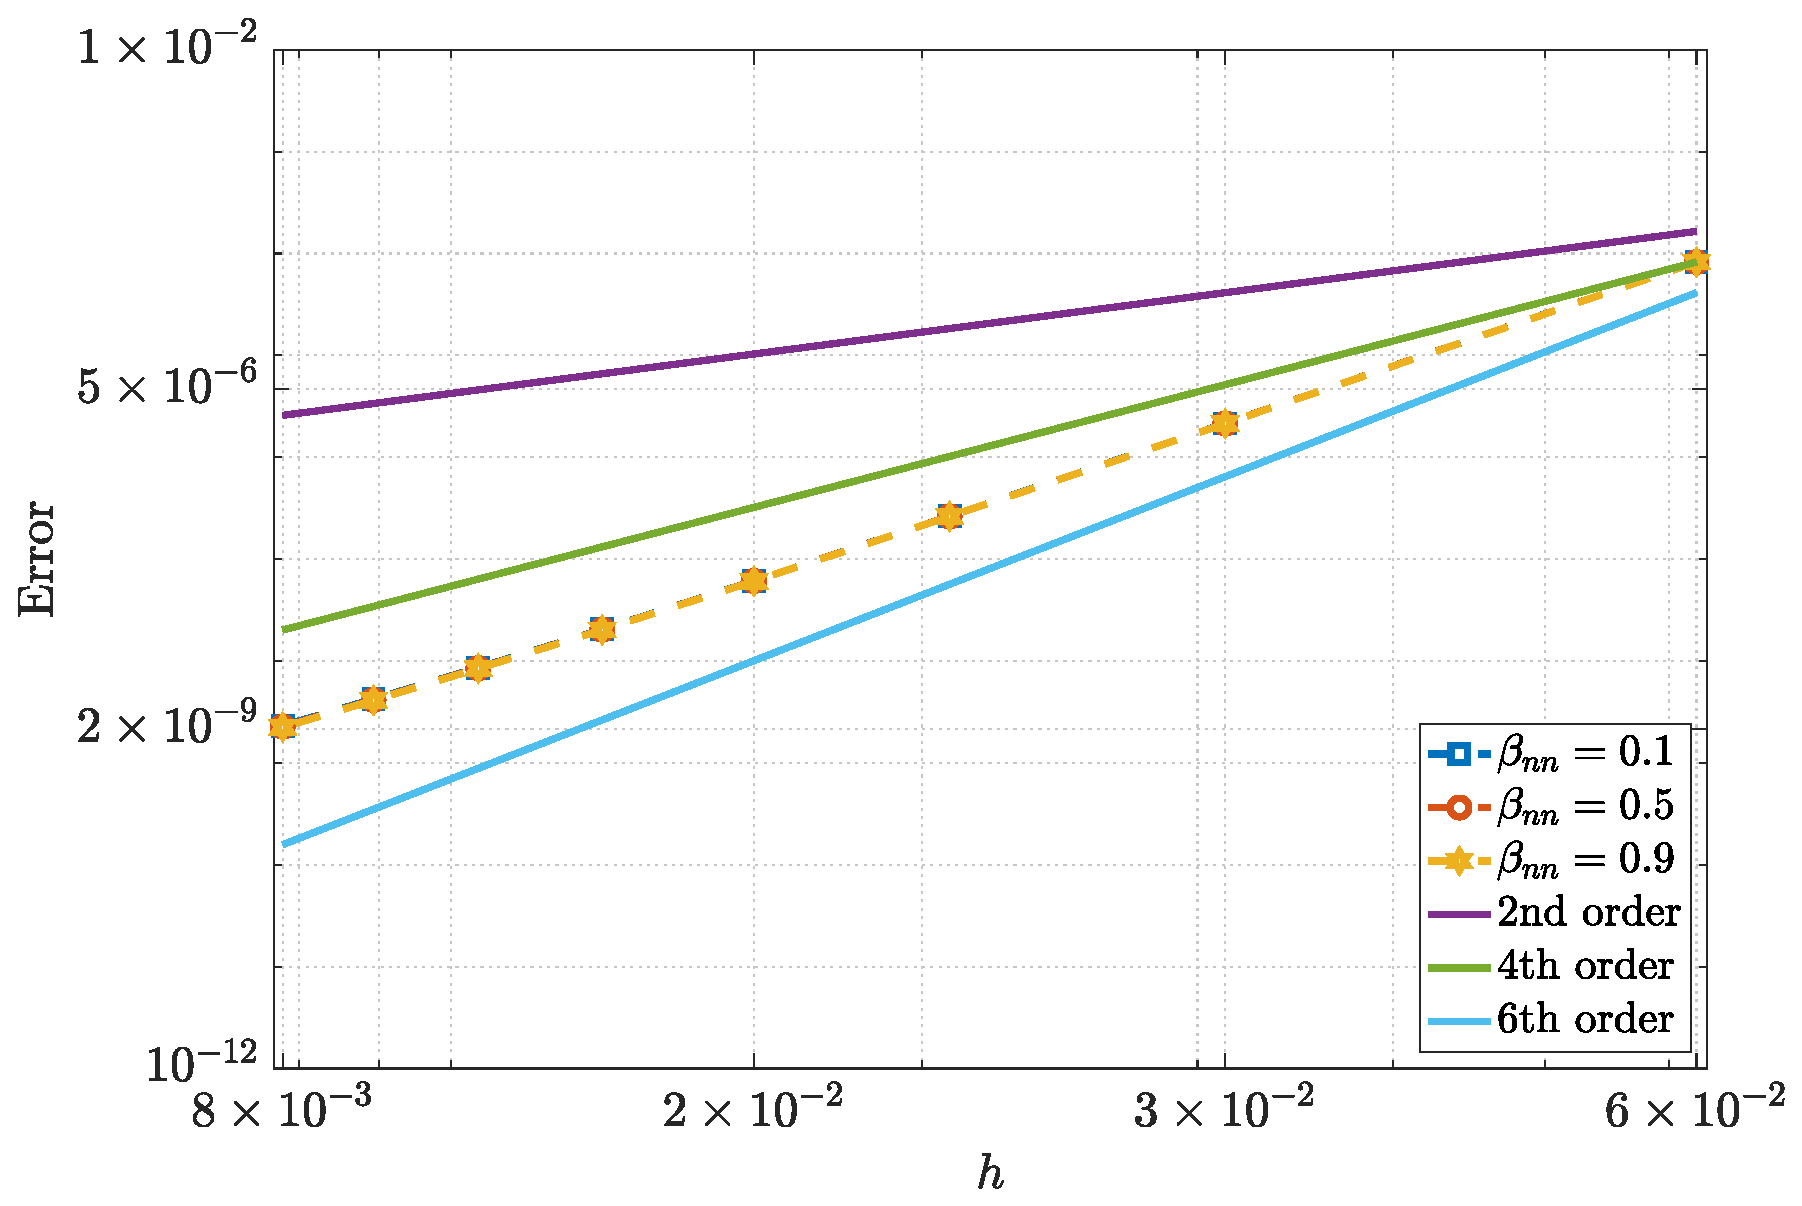
\includegraphics[width=\textwidth]{Figures/NormErr_2nd_Re_100_Wi_1_epsilon_0_xi_0_alphaG_0_Dt_1e-06_at_0.05_tipsim_1_MMS_12_U.eps}
        \captionof{subfigure}{$\overline{u}$}
        \label{oldroydb_u_Case11}
    \end{minipage}
    \hfill
    \begin{minipage}{0.49\textwidth}
        \centering
        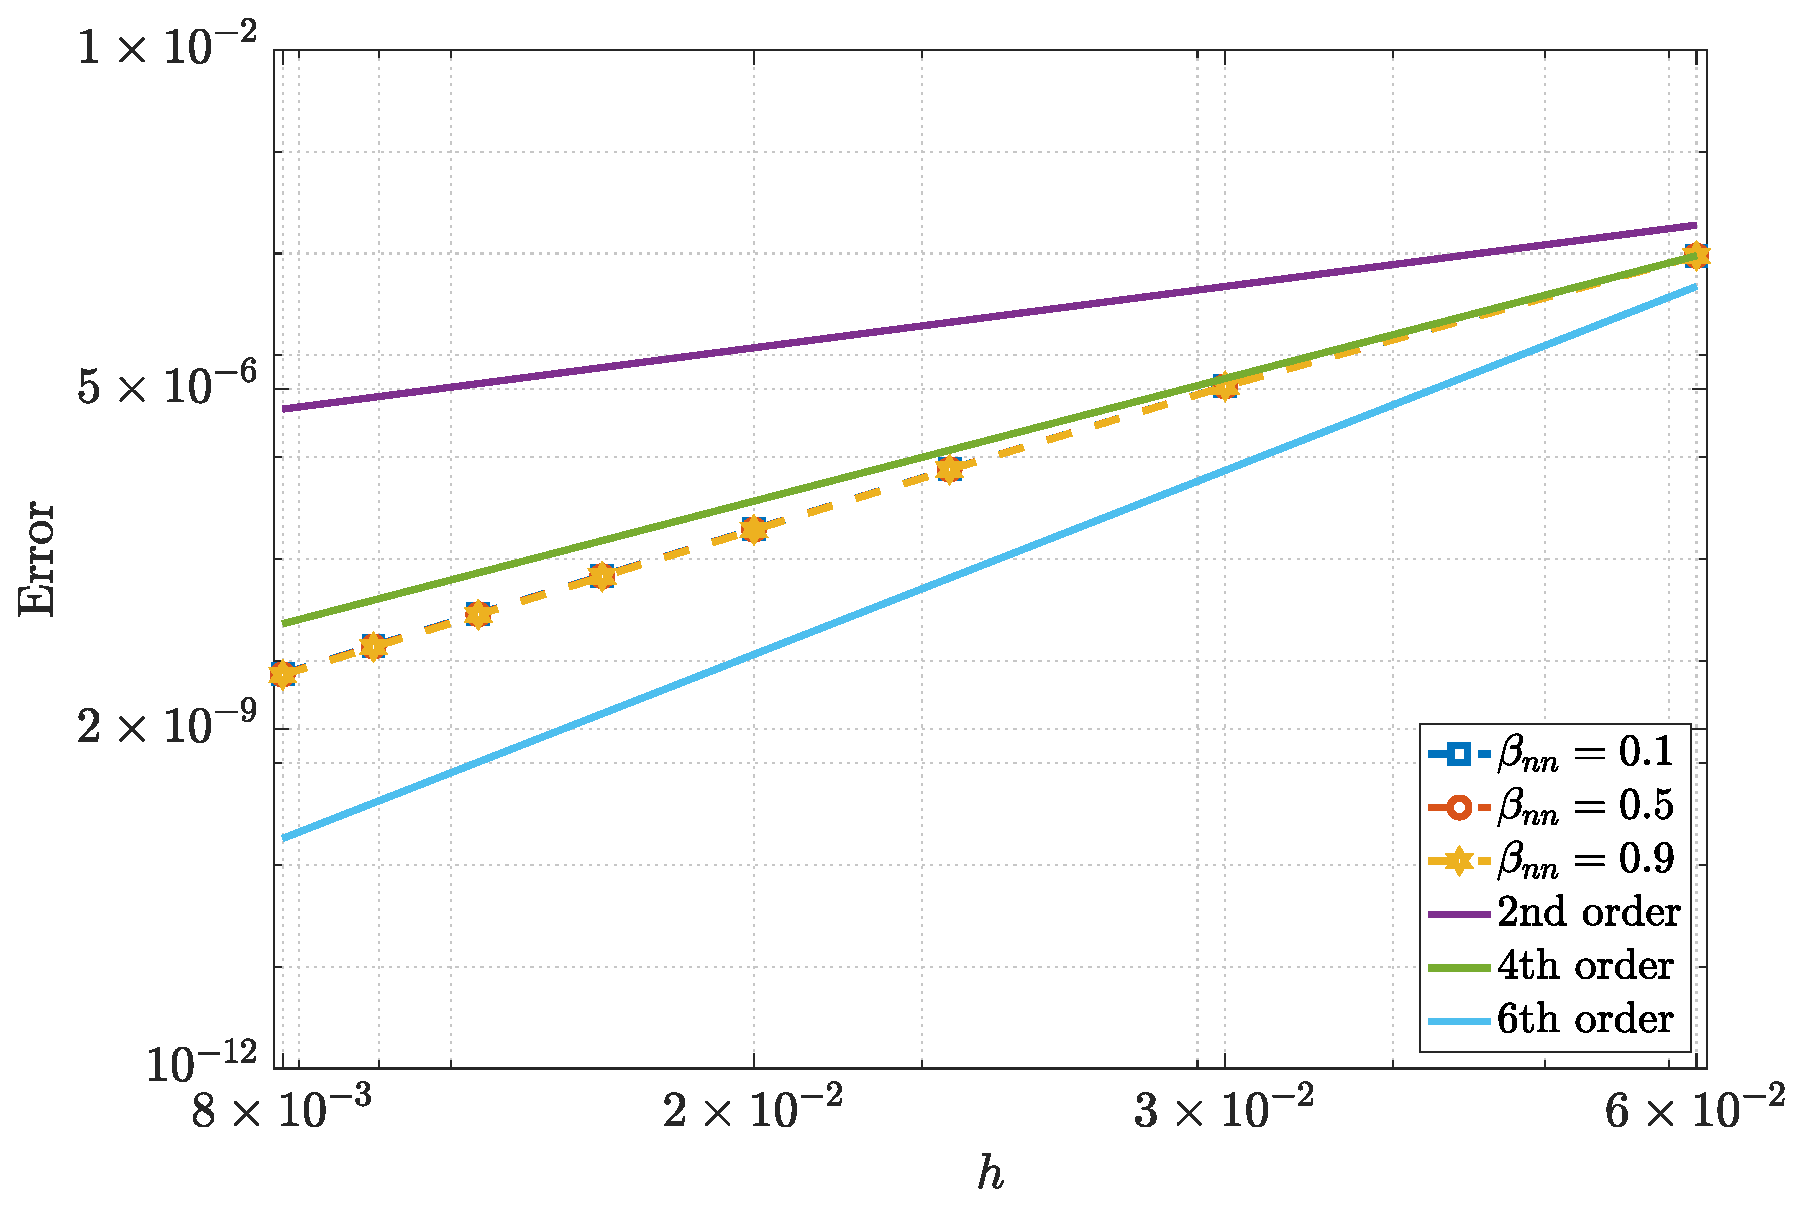
\includegraphics[width=\textwidth]{Figures/NormErr_2nd_Re_100_Wi_1_epsilon_0_xi_0_alphaG_0_Dt_1e-06_at_0.05_tipsim_1_MMS_12_V.eps}
        \captionof{subfigure}{$\tilde{v}$}
        \label{oldroydb_v_Case11}
    \end{minipage}
\end{frame}

%%%%%%%%%%%%%%%%%%%%%%%%%%%%%%%%%%%%%%%%%%%%%%%%%%%%%%%%%%%%%%
\begin{frame}{Caso de verificação usando o modelo Oldroyd-B}
    \centering
    \captionsetup{justification=centering}
    \captionof{figure}{Erro para a vorticidade $(\tilde{\omega_{z}})$ e função de corrente $(\tilde{\psi})$, utilizando $Re=100$ e $Wi=1$ para o escoamento de fluido viscoelástico como o modelo UCM}
    \label{fig:oldroydb_2}
    \begin{minipage}{0.49\textwidth}
        \centering
        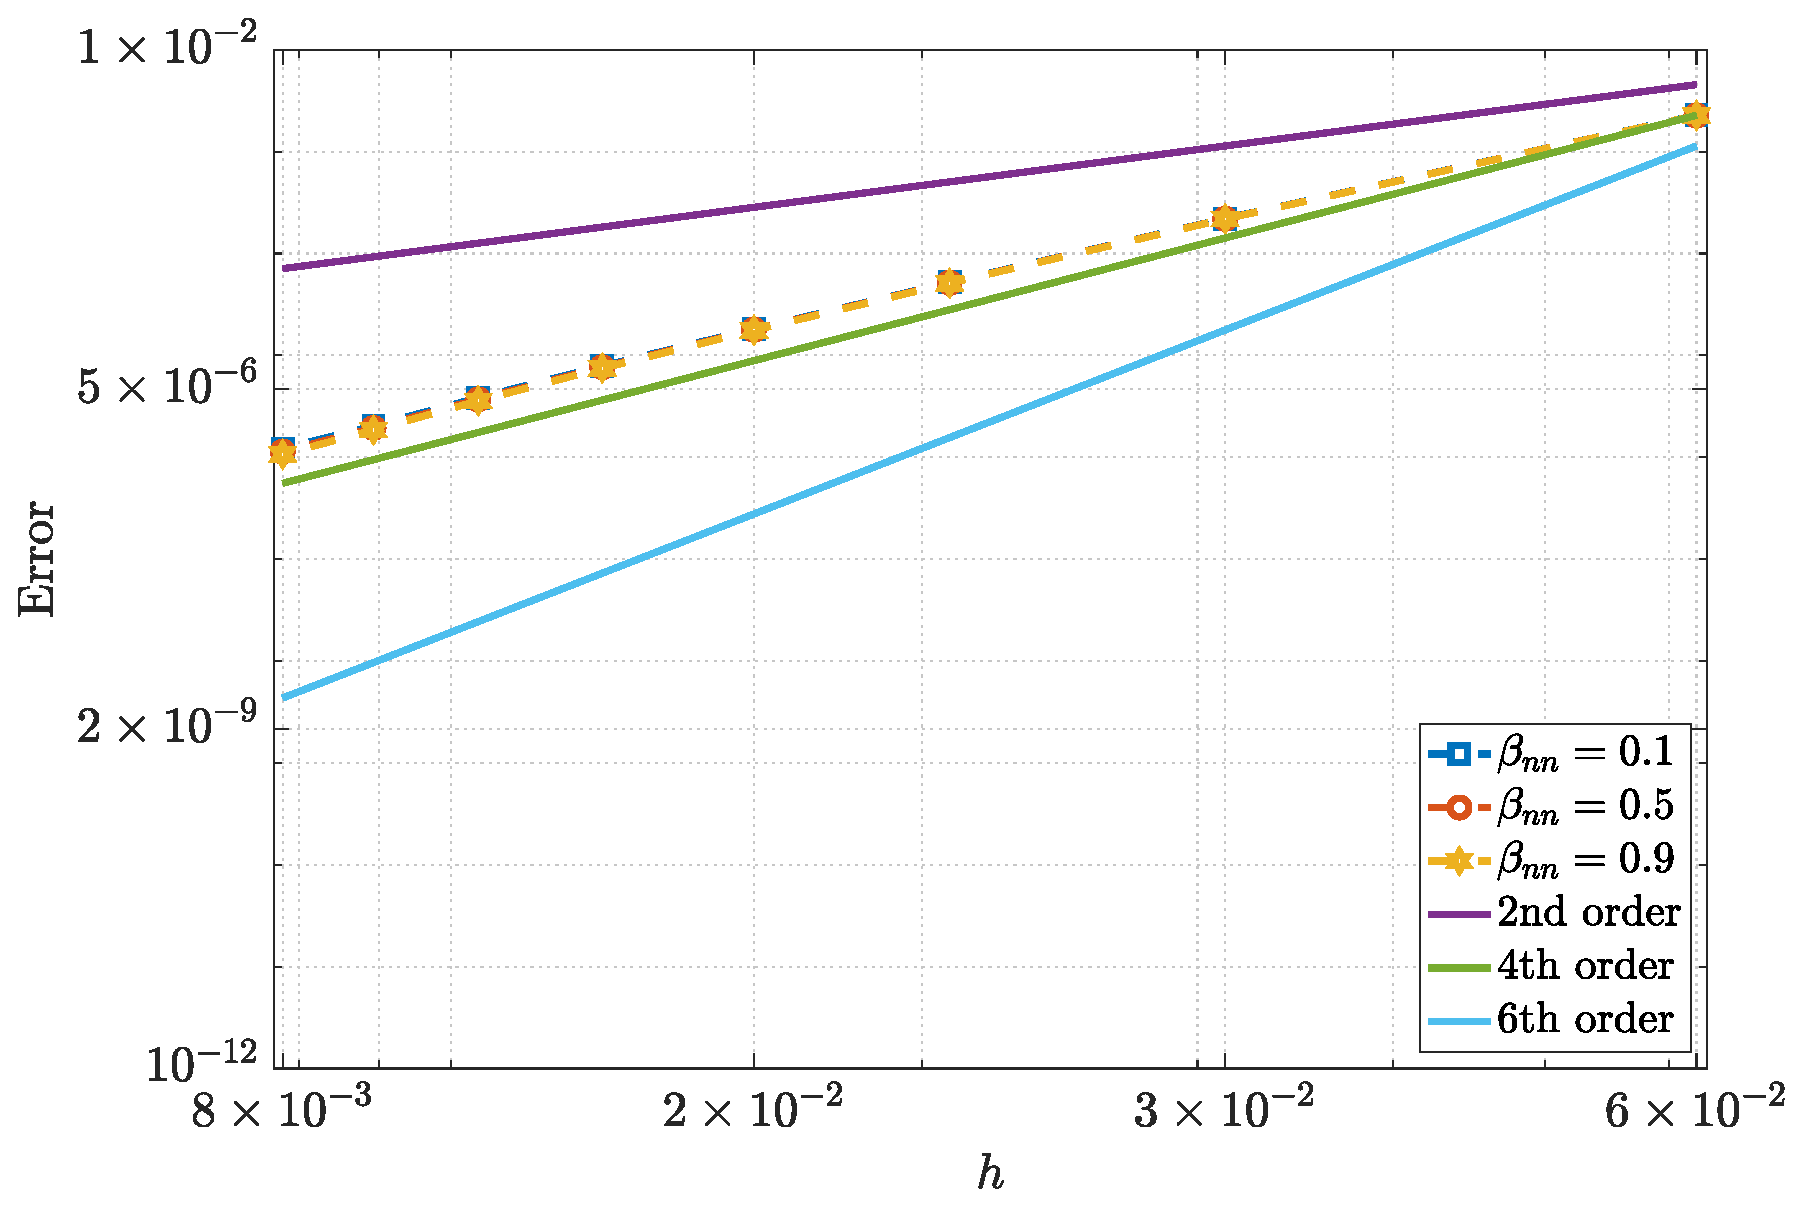
\includegraphics[width=\textwidth]{Figures/NormErr_2nd_Re_100_Wi_1_epsilon_0_xi_0_alphaG_0_Dt_1e-06_at_0.05_tipsim_1_MMS_12_Wz.eps}
        \captionof{subfigure}{$\tilde{\omega_{z}}$}
        \label{oldroydb_wz_Case11}
    \end{minipage}
    \hfill
    \begin{minipage}{0.49\textwidth}
        \centering
        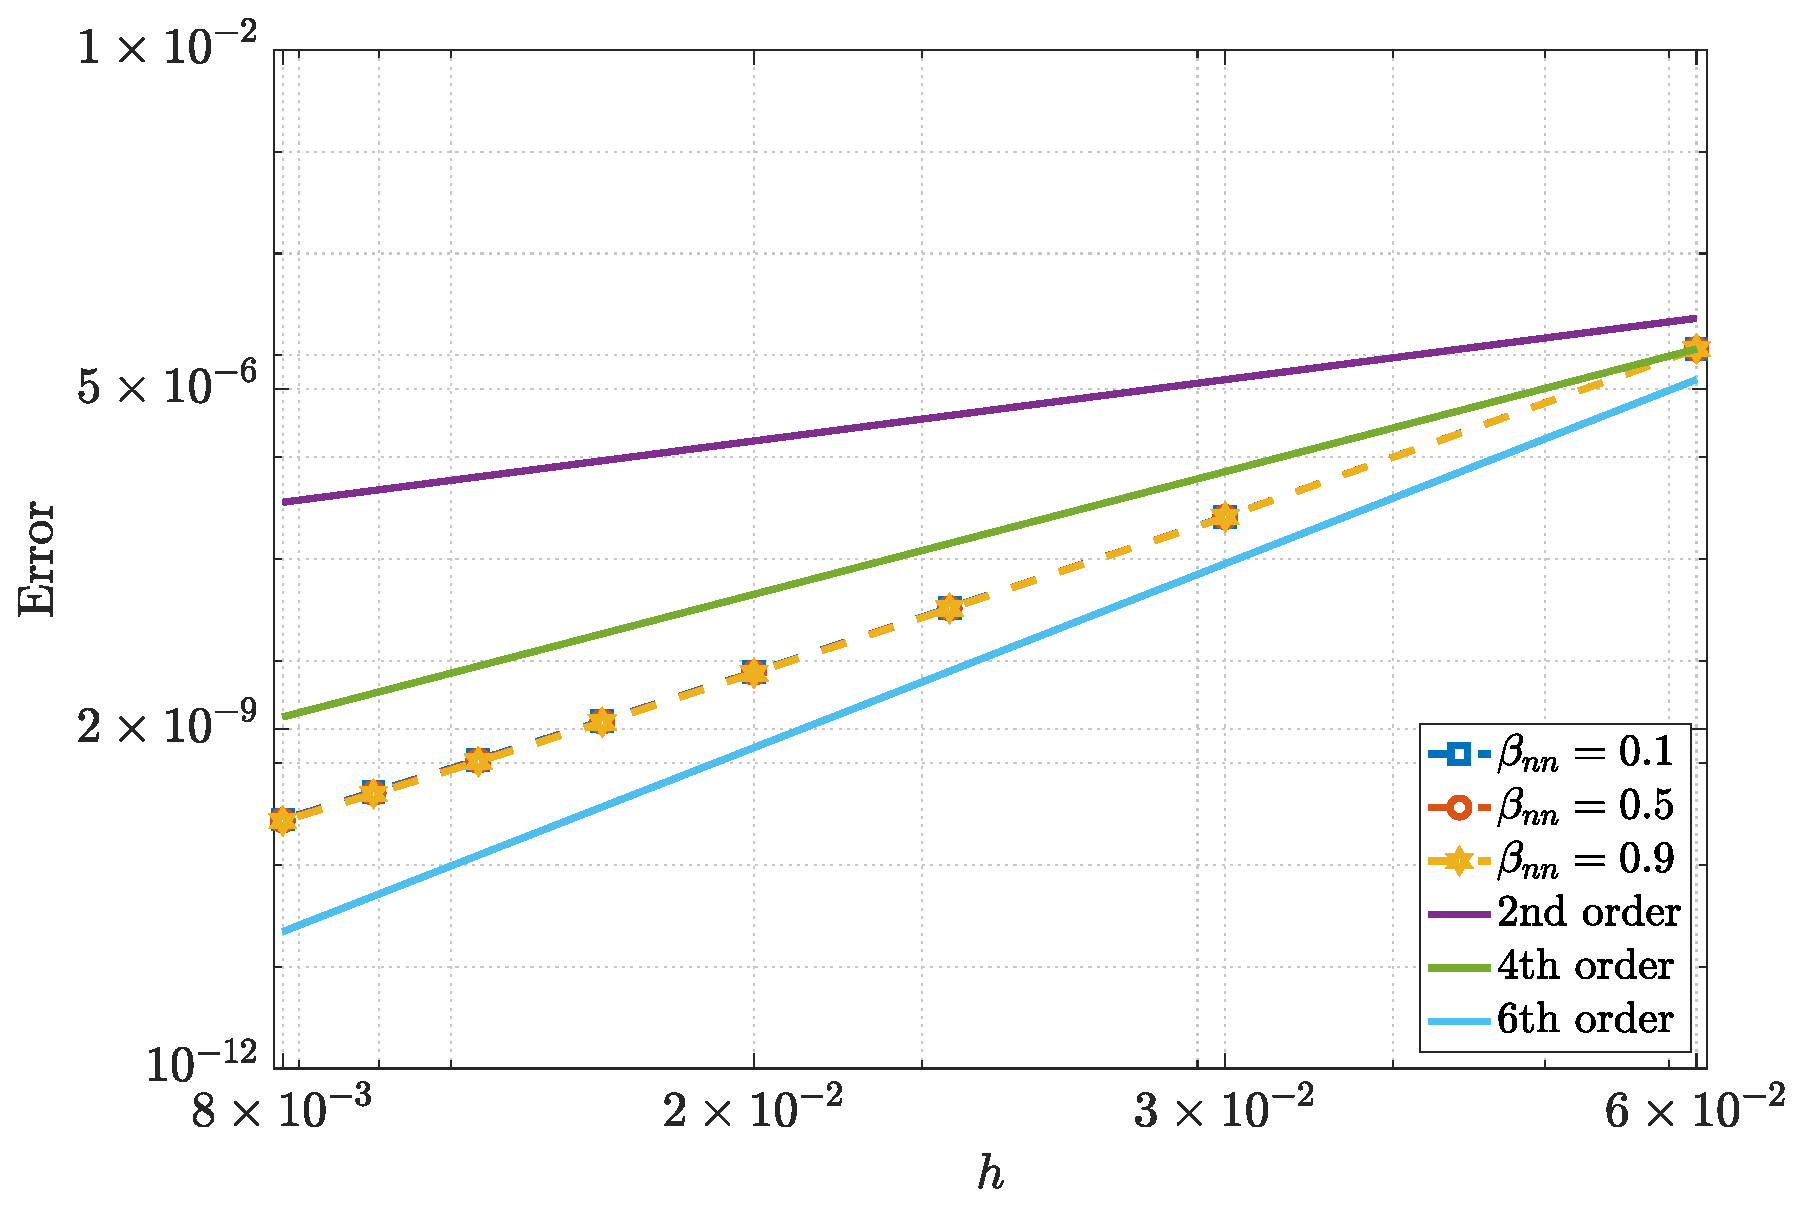
\includegraphics[width=\textwidth]{Figures/NormErr_2nd_Re_100_Wi_1_epsilon_0_xi_0_alphaG_0_Dt_1e-06_at_0.05_tipsim_1_MMS_12_Psi.eps}
        \captionof{subfigure}{$\tilde{\psi}$}
        \label{oldroydb_psi_Case11}
    \end{minipage}
\end{frame}

%%%%%%%%%%%%%%%%%%%%%%%%%%%%%%%%%%%%%%%%%%%%%%%%%%%%%%%%%%%%%%
\begin{frame}{Caso de verificação usando o modelo Oldroyd-B}
    \centering
    \captionsetup{justification=centering}
    \captionof{figure}{Erro para as componentes dos tensores de tensões, utilizando $Re=100$ e $Wi=1$ para o escoamento de fluido viscoelástico como o modelo UCM}
    \label{fig:oldroydb_3}
    \begin{minipage}{0.325\textwidth}
        \centering
        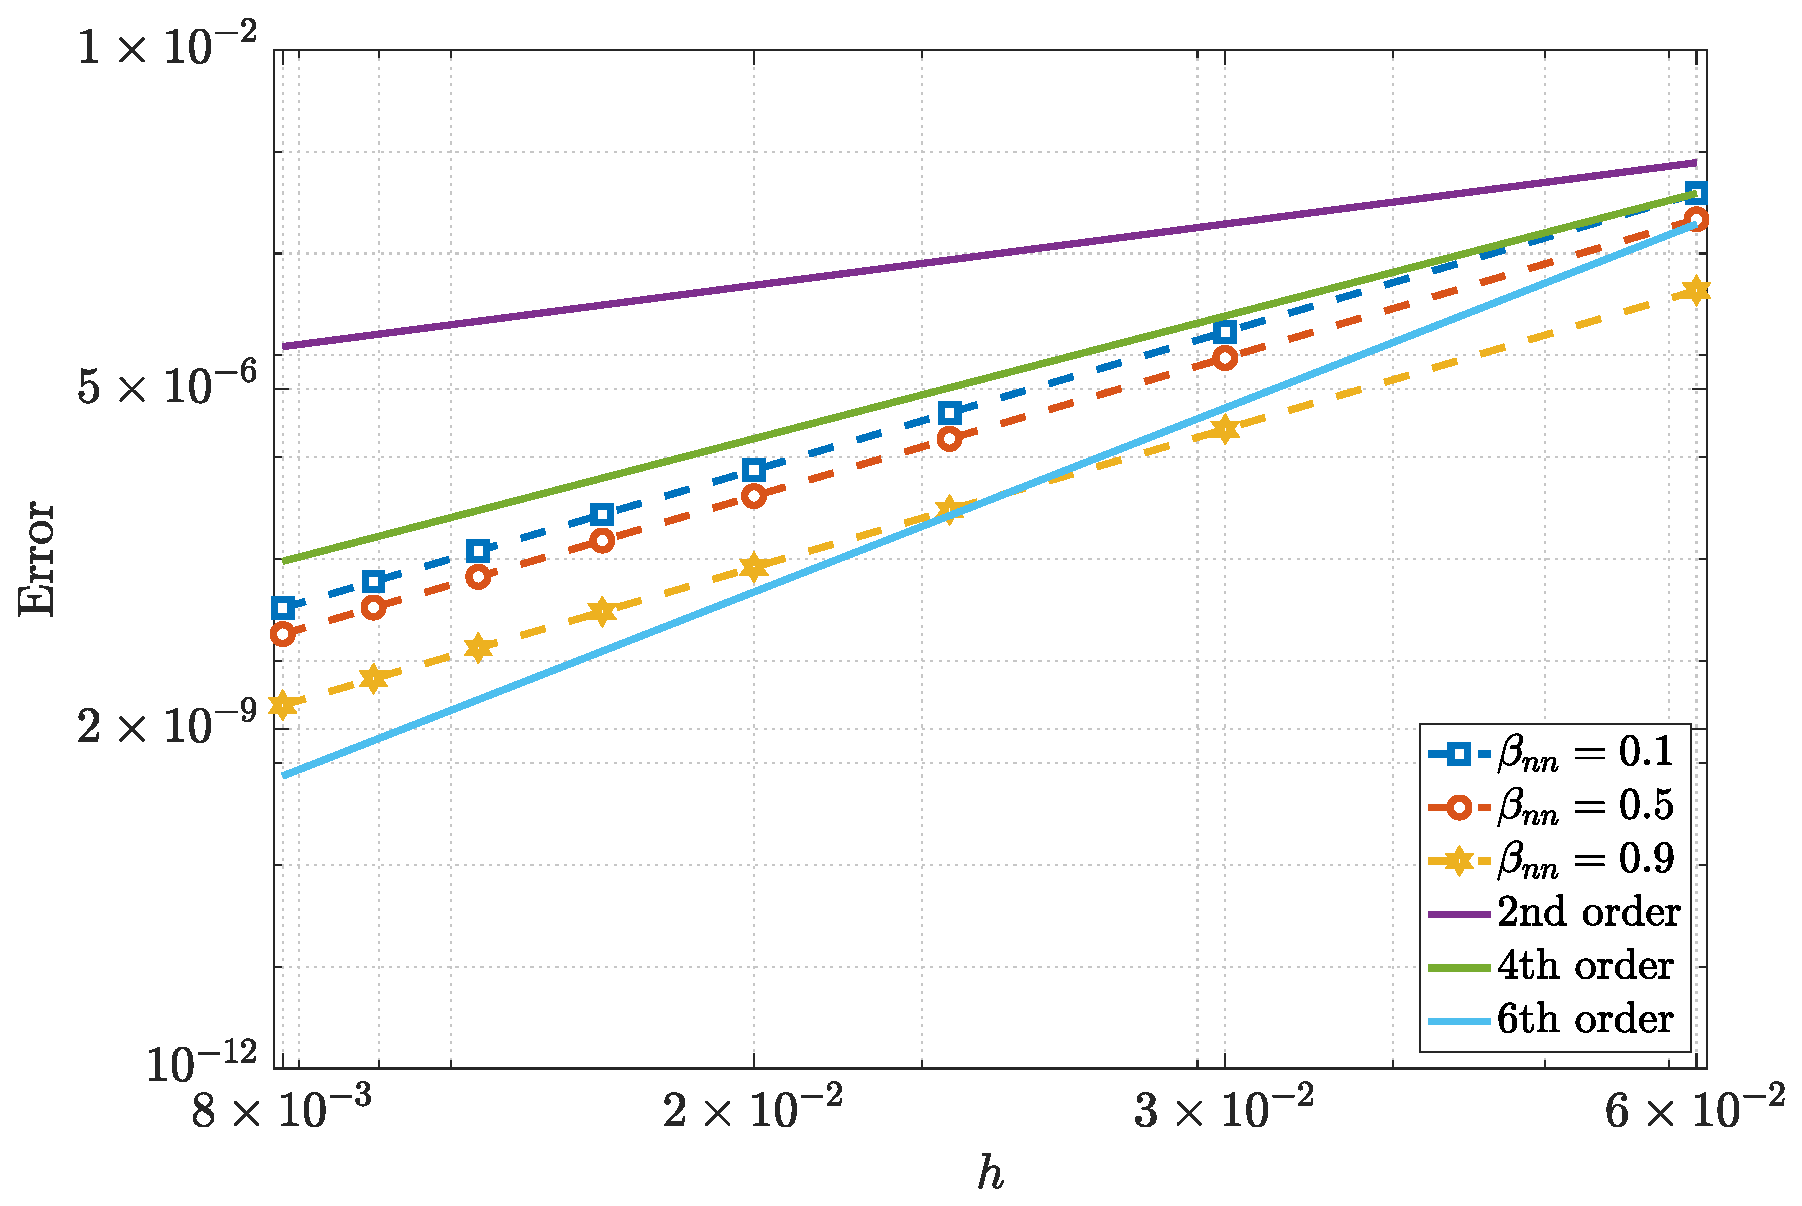
\includegraphics[width=\textwidth]{Figures/NormErr_2nd_Re_100_Wi_1_epsilon_0_xi_0_alphaG_0_Dt_1e-06_at_0.05_tipsim_1_MMS_12_Txx.eps}
        \captionof{subfigure}{$\overline{T_{xx}}$}
        \label{oldroydb_txx_Case11}
    \end{minipage}
    \hfill
    \begin{minipage}{0.325\textwidth}
        \centering
        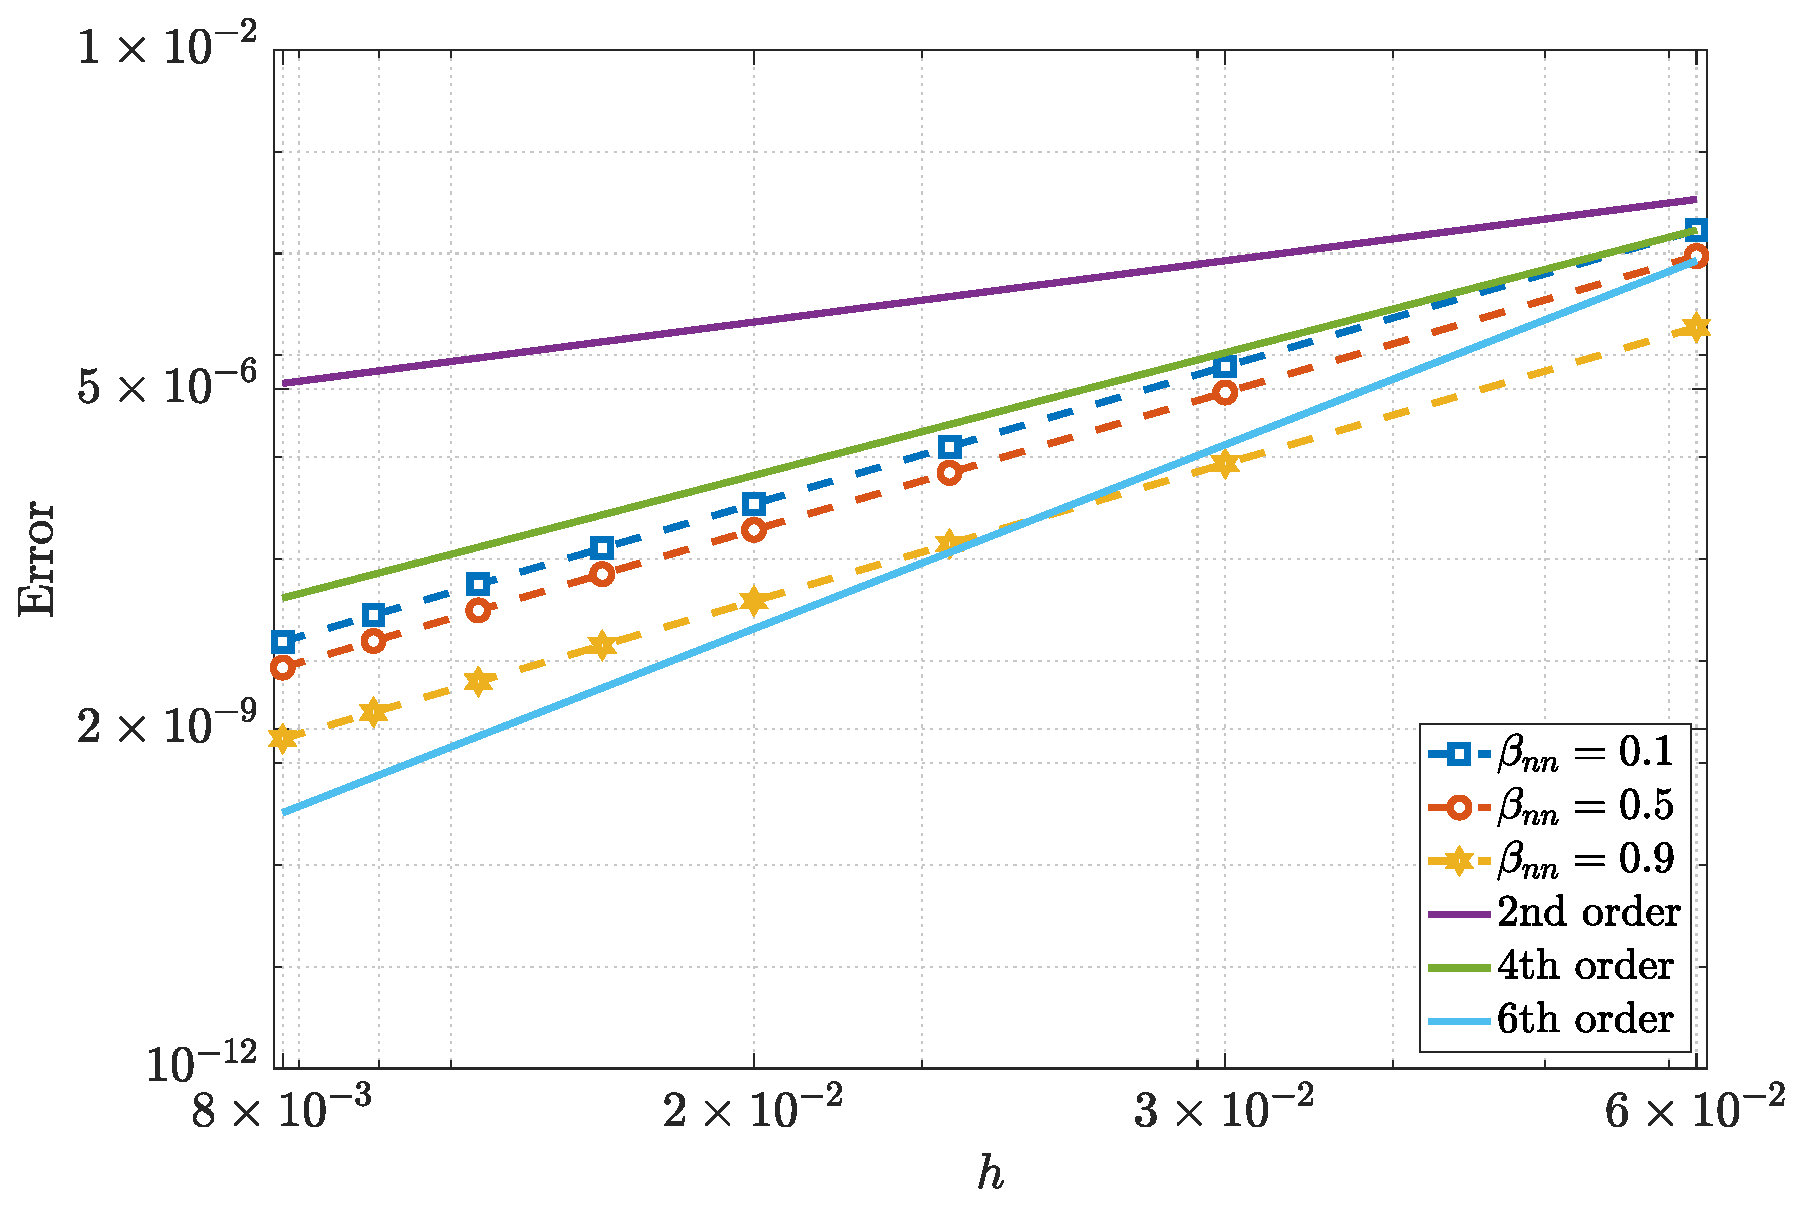
\includegraphics[width=\textwidth]{Figures/NormErr_2nd_Re_100_Wi_1_epsilon_0_xi_0_alphaG_0_Dt_1e-06_at_0.05_tipsim_1_MMS_12_Txy.eps}
        \captionof{subfigure}{$\overline{T_{xy}}$}
        \label{oldroydb_txy_Case11}
    \end{minipage}
    \hfill
    \begin{minipage}{0.325\textwidth}
        \centering
        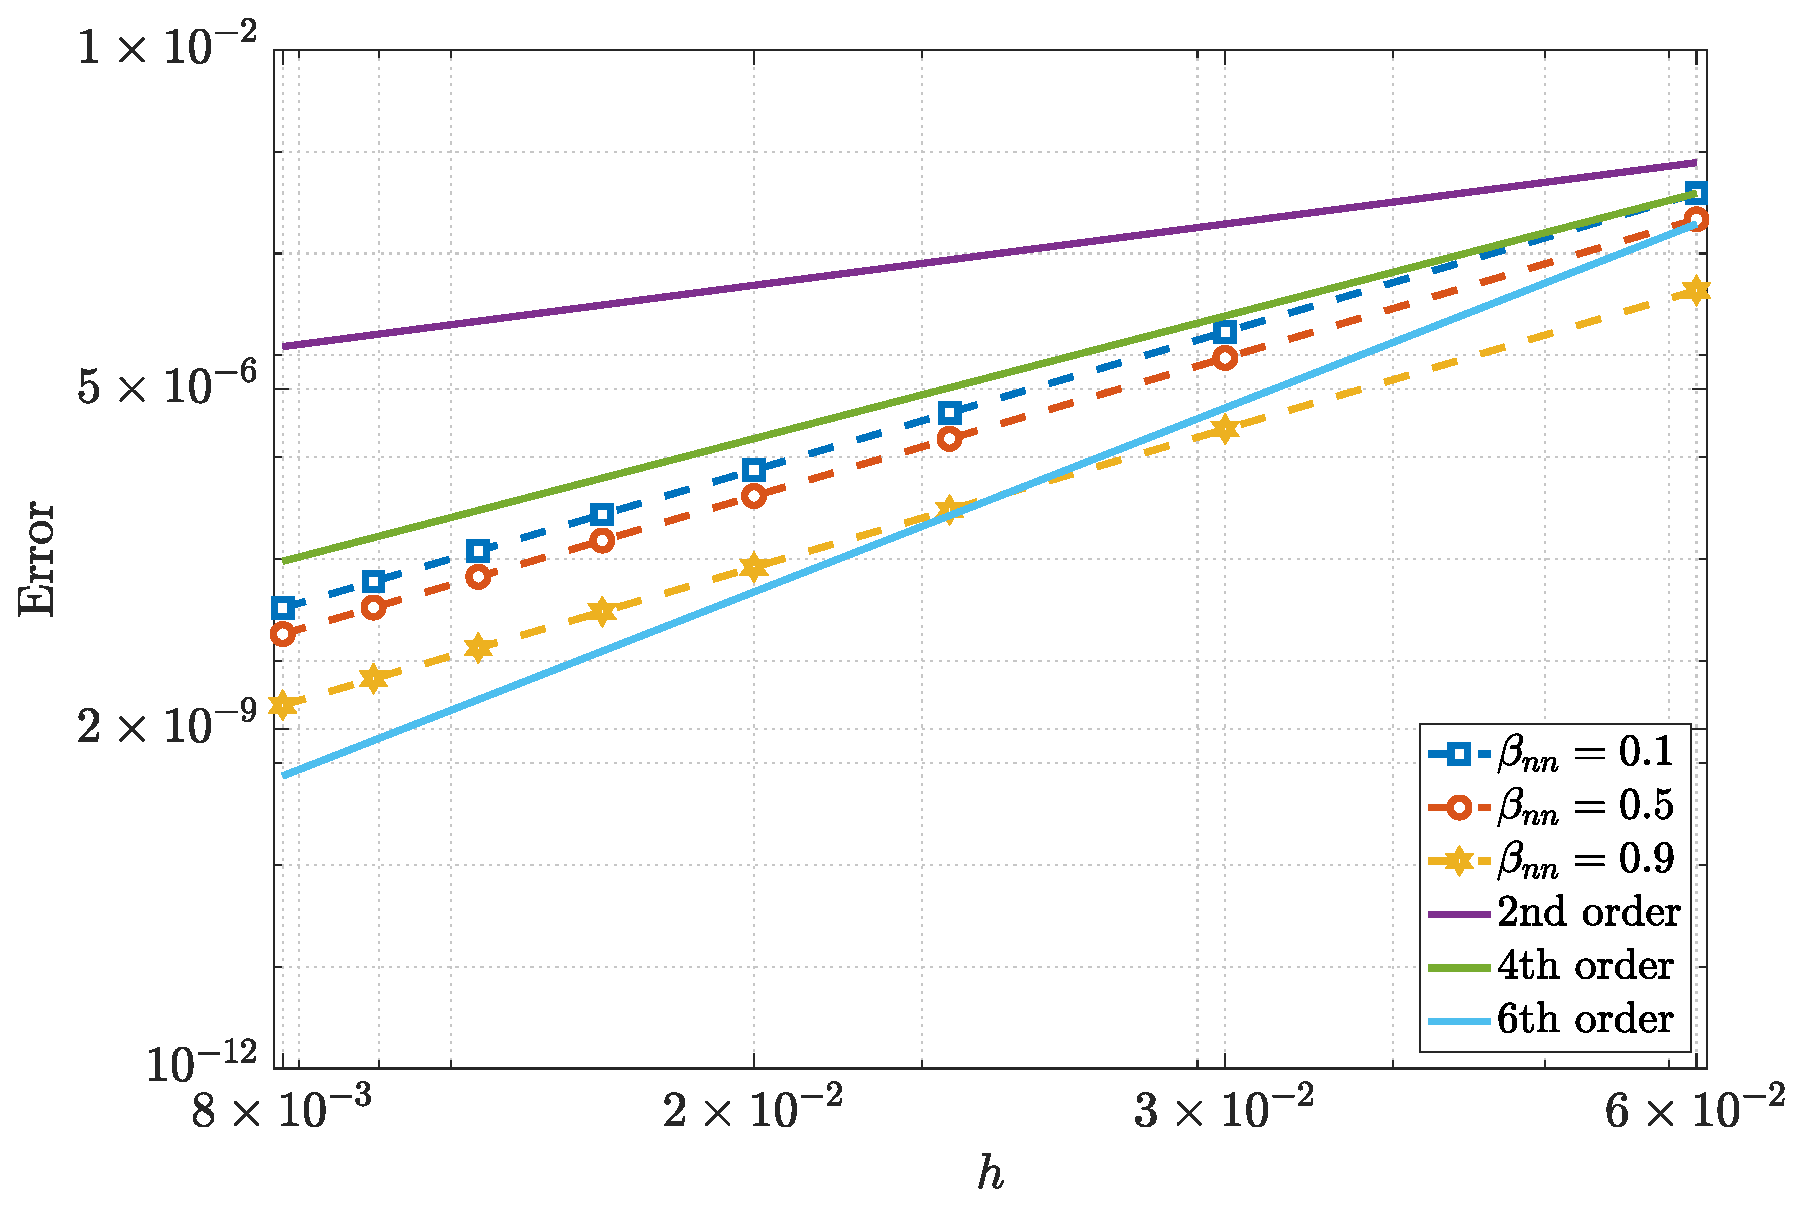
\includegraphics[width=\textwidth]{Figures/NormErr_2nd_Re_100_Wi_1_epsilon_0_xi_0_alphaG_0_Dt_1e-06_at_0.05_tipsim_1_MMS_12_Tyy.eps}
        \captionof{subfigure}{$\overline{T_{yy}}$}
        \label{oldroydb_tyy_Case11}
    \end{minipage}
\end{frame}

%%%%%%%%%%%%%%%%%%%%%%%%%%%%%%%%%%%%%%%%%%%%%%%%%%%%%%%%%%%%%%
\begin{frame}{Caso de verificação usando o modelo Giesekus}
    \centering
    \begin{table}[H]
\caption{Erros numéricos e cálculo da ordem de convergência para a vorticidade $(\omega_{z})$, utilizando o parâmetro $Wi=1$, para o escoamento de fluido viscoelástico Giesekus.\label{tab_GiesekusWzResumida_1}}
\scriptsize{
    \begin{tabular*}{\textwidth}{@{\extracolsep\fill}cccccccccc@{}}
    \hline
    \multirow{2}{*}{$\operatorname{Re}$} & \multirow{2}{*}{Malha} & \multicolumn{2}{c}{$\beta_{nn}=0.1$}  & \multicolumn{2}{c}{$\beta_{nn}=0.5$}  & \multicolumn{2}{c}{$\beta_{nn}=0.9$}  & \multicolumn{2}{c}{$\beta_{nn}=1.0$}\\ %\cline{2-10}
     & & Erro & Ordem & Erro & Ordem & Erro & Ordem & Erro & Ordem \\
    \hline
    \multirow{7}{*}{1.00} & $17\times 17$ & 2.23e-03 & --- & 2.08e-03 & --- & 1.96e-03 & --- & 1.93e-03 & --- \\
    & $33\times 33$ & 2.02e-04 & 3.47 & 1.51e-04 & 3.79 & 1.23e-04 & 4.00 & 1.18e-04 & 4.03 \\
    & $49\times 49$ & 4.26e-05 & 3.84 & 2.50e-05 & 4.44 & 1.92e-05 & 4.57 & 1.84e-05 & 4.58 \\
    & $65\times 65$ & 1.28e-05 & 4.17 & 6.43e-06 & 4.71 & 5.05e-06 & 4.65 & 4.85e-06 & 4.63 \\
    & $81\times 81$ & 4.68e-06 & 4.52 & 2.23e-06 & 4.74 & 1.79e-06 & 4.63 & 1.73e-06 & 4.61 \\
    & $97\times 97$ & 1.92e-06 & 4.90 & 9.34e-07 & 4.78 & 7.68e-07 & 4.65 & 7.45e-07 & 4.63 \\
    & $113\times 113$ & 8.58e-07 & 5.21 & 4.47e-07 & 4.77 & 3.80e-07 & 4.57 & 3.71e-07 & 4.52 \\
    & $129\times 129$ & 4.34e-07 & 5.10 & 2.59e-07 & 4.11 & 2.30e-07 & 3.76 & 2.26e-07 & 3.71 \\
    \hline
    \multirow{7}{*}{100.00} & $17\times 17$ & 2.27e-03 & --- & 2.27e-03 & --- & 2.26e-03 & --- & 2.26e-03 & --- \\
    & $33\times 33$ & 2.20e-04 & 3.37 & 2.19e-04 & 3.37 & 2.18e-04 & 3.37 & 2.18e-04 & 3.37 \\
    & $49\times 49$ & 5.20e-05 & 3.56 & 5.15e-05 & 3.57 & 5.11e-05 & 3.58 & 5.10e-05 & 3.59 \\
    & $65\times 65$ & 1.82e-05 & 3.66 & 1.79e-05 & 3.68 & 1.76e-05 & 3.70 & 1.75e-05 & 3.71 \\
    & $81\times 81$ & 7.84e-06 & 3.76 & 7.65e-06 & 3.80 & 7.47e-06 & 3.84 & 7.43e-06 & 3.85 \\
    & $97\times 97$ & 3.83e-06 & 3.93 & 3.70e-06 & 3.99 & 3.57e-06 & 4.05 & 3.54e-06 & 4.06 \\
    & $113\times 113$ & 2.04e-06 & 4.10 & 1.94e-06 & 4.19 & 1.85e-06 & 4.27 & 1.83e-06 & 4.29 \\
    & $129\times 129$ & 1.21e-06 & 3.89 & 1.13e-06 & 4.02 & 1.07e-06 & 4.13 & 1.05e-06 & 4.16 \\
    \hline
    \end{tabular*}
}
\end{table}
\end{frame}

%%%%%%%%%%%%%%%%%%%%%%%%%%%%%%%%%%%%%%%%%%%%%%%%%%%%%%%%%%%%%%
\begin{frame}{Caso de verificação usando o modelo Giesekus}
    \centering
    \begin{table}[H]
\caption{Erros numéricos e cálculo da ordem de convergência para a vorticidade $(\omega_{z})$, utilizando o parâmetro $Wi=1$, para o escoamento de fluido viscoelástico Giesekus.\label{tab_GiesekusWzResumida_2}}
\scriptsize{
    \begin{tabular*}{\textwidth}{@{\extracolsep\fill}cccccccccc@{}}
    \hline
    \multirow{2}{*}{$\operatorname{Re}$} & \multirow{2}{*}{Malha} & \multicolumn{2}{c}{$\beta_{nn}=0.1$}  & \multicolumn{2}{c}{$\beta_{nn}=0.5$}  & \multicolumn{2}{c}{$\beta_{nn}=0.9$}  & \multicolumn{2}{c}{$\beta_{nn}=1.0$}\\ %\cline{2-10}
     & & Erro & Ordem & Erro & Ordem & Erro & Ordem & Erro & Ordem \\
    \hline
    \multirow{7}{*}{400.00} & $17\times 17$ & 2.27e-03 & --- & 2.27e-03 & --- & 2.27e-03 & --- & 2.27e-03 & --- \\
    & $33\times 33$ & 2.20e-04 & 3.37 & 2.20e-04 & 3.37 & 2.20e-04 & 3.37 & 2.20e-04 & 3.37 \\
    & $49\times 49$ & 5.21e-05 & 3.56 & 5.19e-05 & 3.56 & 5.18e-05 & 3.56 & 5.18e-05 & 3.56 \\
    & $65\times 65$ & 1.82e-05 & 3.65 & 1.81e-05 & 3.66 & 1.81e-05 & 3.66 & 1.81e-05 & 3.66 \\
    & $81\times 81$ & 7.88e-06 & 3.75 & 7.83e-06 & 3.76 & 7.79e-06 & 3.77 & 7.78e-06 & 3.77 \\
    & $97\times 97$ & 3.86e-06 & 3.92 & 3.83e-06 & 3.93 & 3.80e-06 & 3.94 & 3.79e-06 & 3.95 \\
    & $113\times 113$ & 2.05e-06 & 4.09 & 2.03e-06 & 4.11 & 2.01e-06 & 4.12 & 2.01e-06 & 4.13 \\
    & $129\times 129$ & 1.23e-06 & 3.86 & 1.21e-06 & 3.89 & 1.19e-06 & 3.92 & 1.19e-06 & 3.93 \\
    \hline
    \multirow{7}{*}{1000.00} & $17\times 17$ & 2.27e-03 & --- & 2.27e-03 & --- & 2.27e-03 & --- & 2.27e-03 & --- \\
    & $33\times 33$ & 2.20e-04 & 3.37 & 2.20e-04 & 3.37 & 2.20e-04 & 3.37 & 2.20e-04 & 3.37 \\
    & $49\times 49$ & 5.21e-05 & 3.56 & 5.20e-05 & 3.56 & 5.20e-05 & 3.56 & 5.20e-05 & 3.56 \\
    & $65\times 65$ & 1.82e-05 & 3.65 & 1.82e-05 & 3.65 & 1.82e-05 & 3.65 & 1.82e-05 & 3.65 \\
    & $81\times 81$ & 7.89e-06 & 3.75 & 7.87e-06 & 3.76 & 7.86e-06 & 3.76 & 7.85e-06 & 3.76 \\
    & $97\times 97$ & 3.86e-06 & 3.92 & 3.85e-06 & 3.92 & 3.84e-06 & 3.92 & 3.84e-06 & 3.92 \\
    & $113\times 113$ & 2.06e-06 & 4.08 & 2.05e-06 & 4.09 & 2.04e-06 & 4.09 & 2.04e-06 & 4.09 \\
    & $129\times 129$ & 1.23e-06 & 3.86 & 1.22e-06 & 3.87 & 1.22e-06 & 3.87 & 1.22e-06 & 3.88 \\
    \hline
    \end{tabular*}
}
\end{table}
\end{frame}

%%%%%%%%%%%%%%%%%%%%%%%%%%%%%%%%%%%%%%%%%%%%%%%%%%%%%%%%%%%%%%
\begin{frame}{Caso de verificação usando o modelo Giesekus}
    \centering
    \captionsetup{justification=centering}
    \captionof{figure}{Erro para o campo de velocidades $(\overline{u},\tilde{v})$ utilizando $Re=100$, $Wi=1$ e $\alpha_G=0.1$ para o escoamento de fluido viscoelástico como o modelo Giesekus}
    \label{fig:giesekus_1}
    \begin{minipage}{0.49\textwidth}
        \centering
        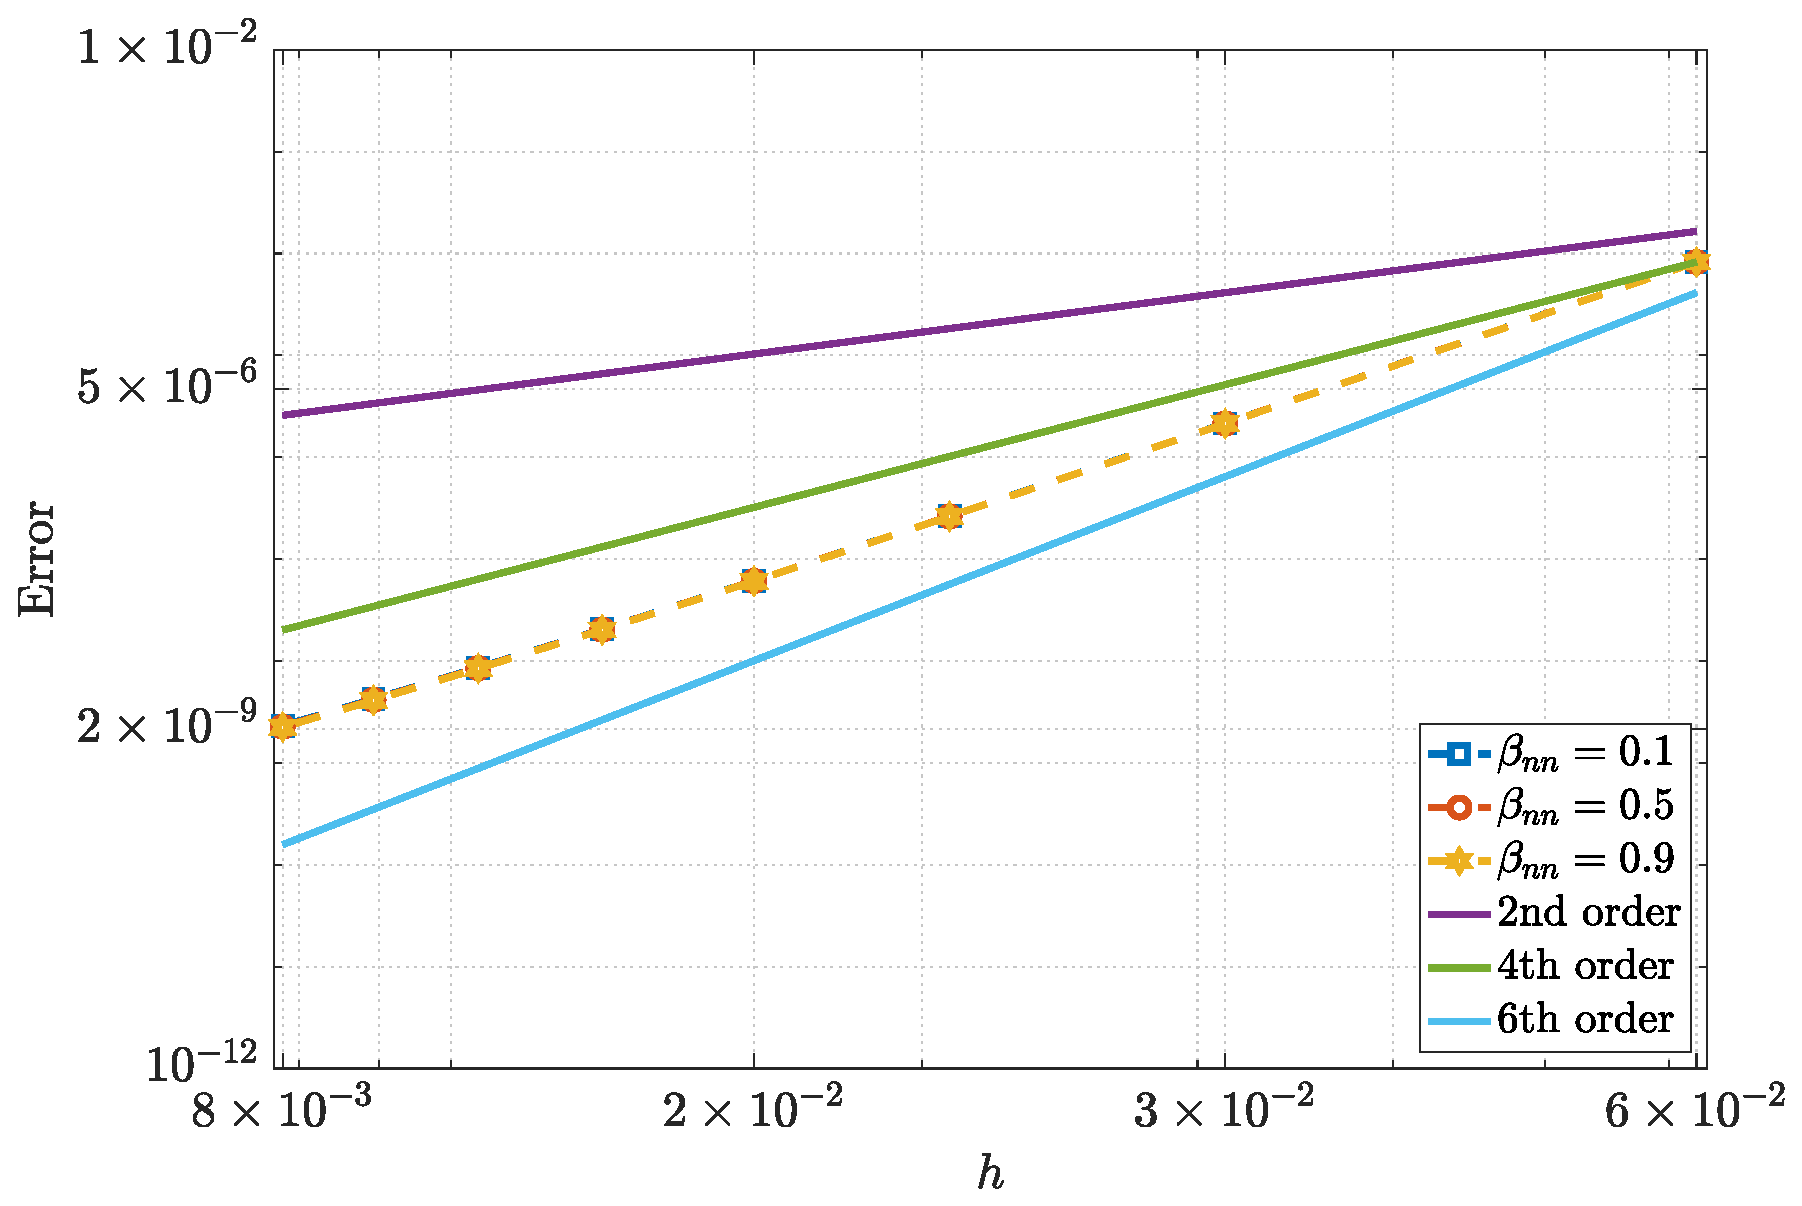
\includegraphics[width=\textwidth]{Figures/NormErr_2nd_Re_100_Wi_1_epsilon_0_xi_0_alphaG_0.1_Dt_1e-06_at_0.05_tipsim_1_MMS_12_U.eps}
        \captionof{subfigure}{$\overline{u}$}
        \label{giesekus_u_Case11}
    \end{minipage}
    \hfill
    \begin{minipage}{0.49\textwidth}
        \centering
        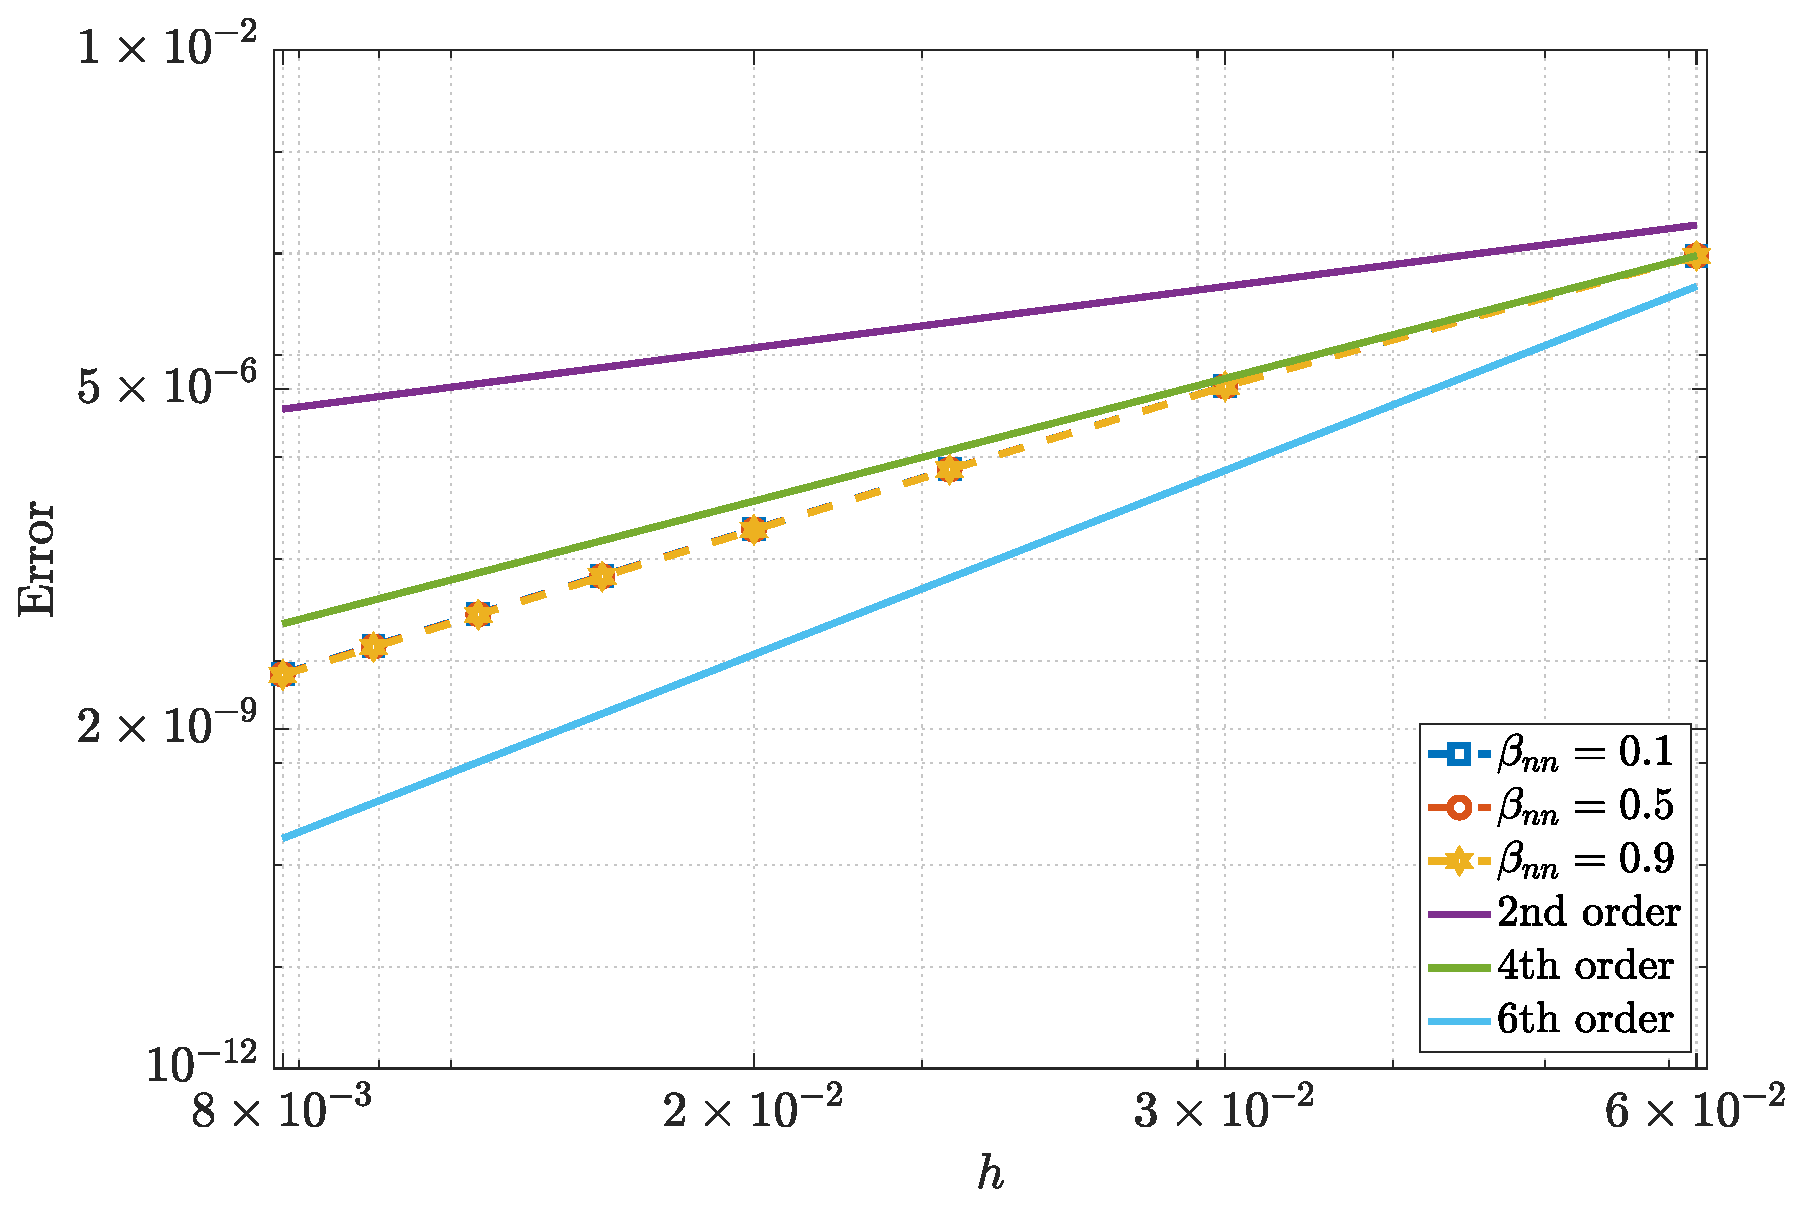
\includegraphics[width=\textwidth]{Figures/NormErr_2nd_Re_100_Wi_1_epsilon_0_xi_0_alphaG_0.1_Dt_1e-06_at_0.05_tipsim_1_MMS_12_V.eps}
        \captionof{subfigure}{$\tilde{v}$}
        \label{giesekus_v_Case11}
    \end{minipage}
\end{frame}

%%%%%%%%%%%%%%%%%%%%%%%%%%%%%%%%%%%%%%%%%%%%%%%%%%%%%%%%%%%%%%
\begin{frame}{Caso de verificação usando o modelo Giesekus}
    \centering
    \captionsetup{justification=centering}
    \captionof{figure}{Erro para a vorticidade $(\tilde{\omega_{z}})$ e função de corrente $(\tilde{\psi})$, utilizando $Re=100$, $Wi=1$ e $\alpha_G=0.1$ para o escoamento de fluido viscoelástico como o modelo Giesekus}
    \label{fig:giesekus_2}
    \begin{minipage}{0.49\textwidth}
        \centering
        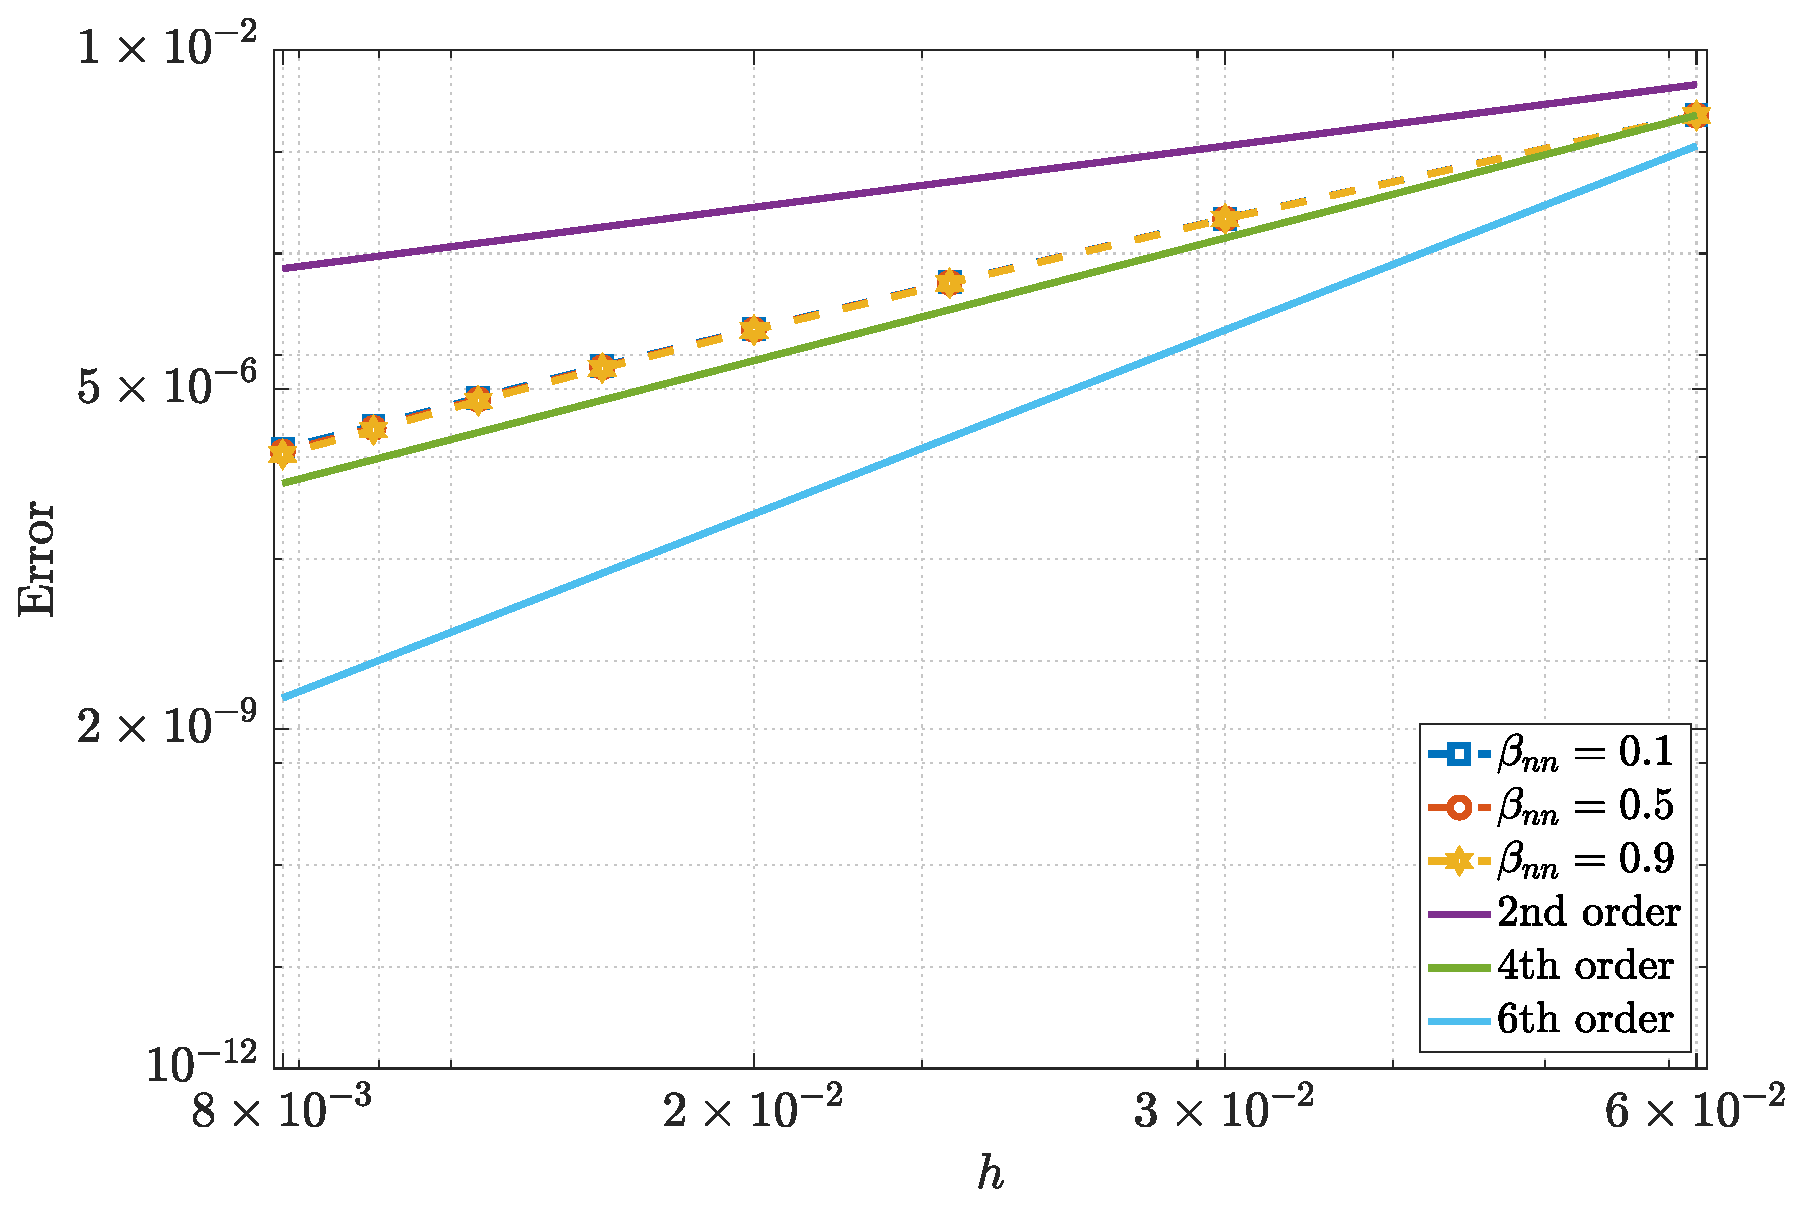
\includegraphics[width=\textwidth]{Figures/NormErr_2nd_Re_100_Wi_1_epsilon_0_xi_0_alphaG_0.1_Dt_1e-06_at_0.05_tipsim_1_MMS_12_Wz.eps}
        \captionof{subfigure}{$\tilde{\omega_{z}}$}
        \label{giesekus_wz_Case11}
    \end{minipage}
    \hfill
    \begin{minipage}{0.49\textwidth}
        \centering
        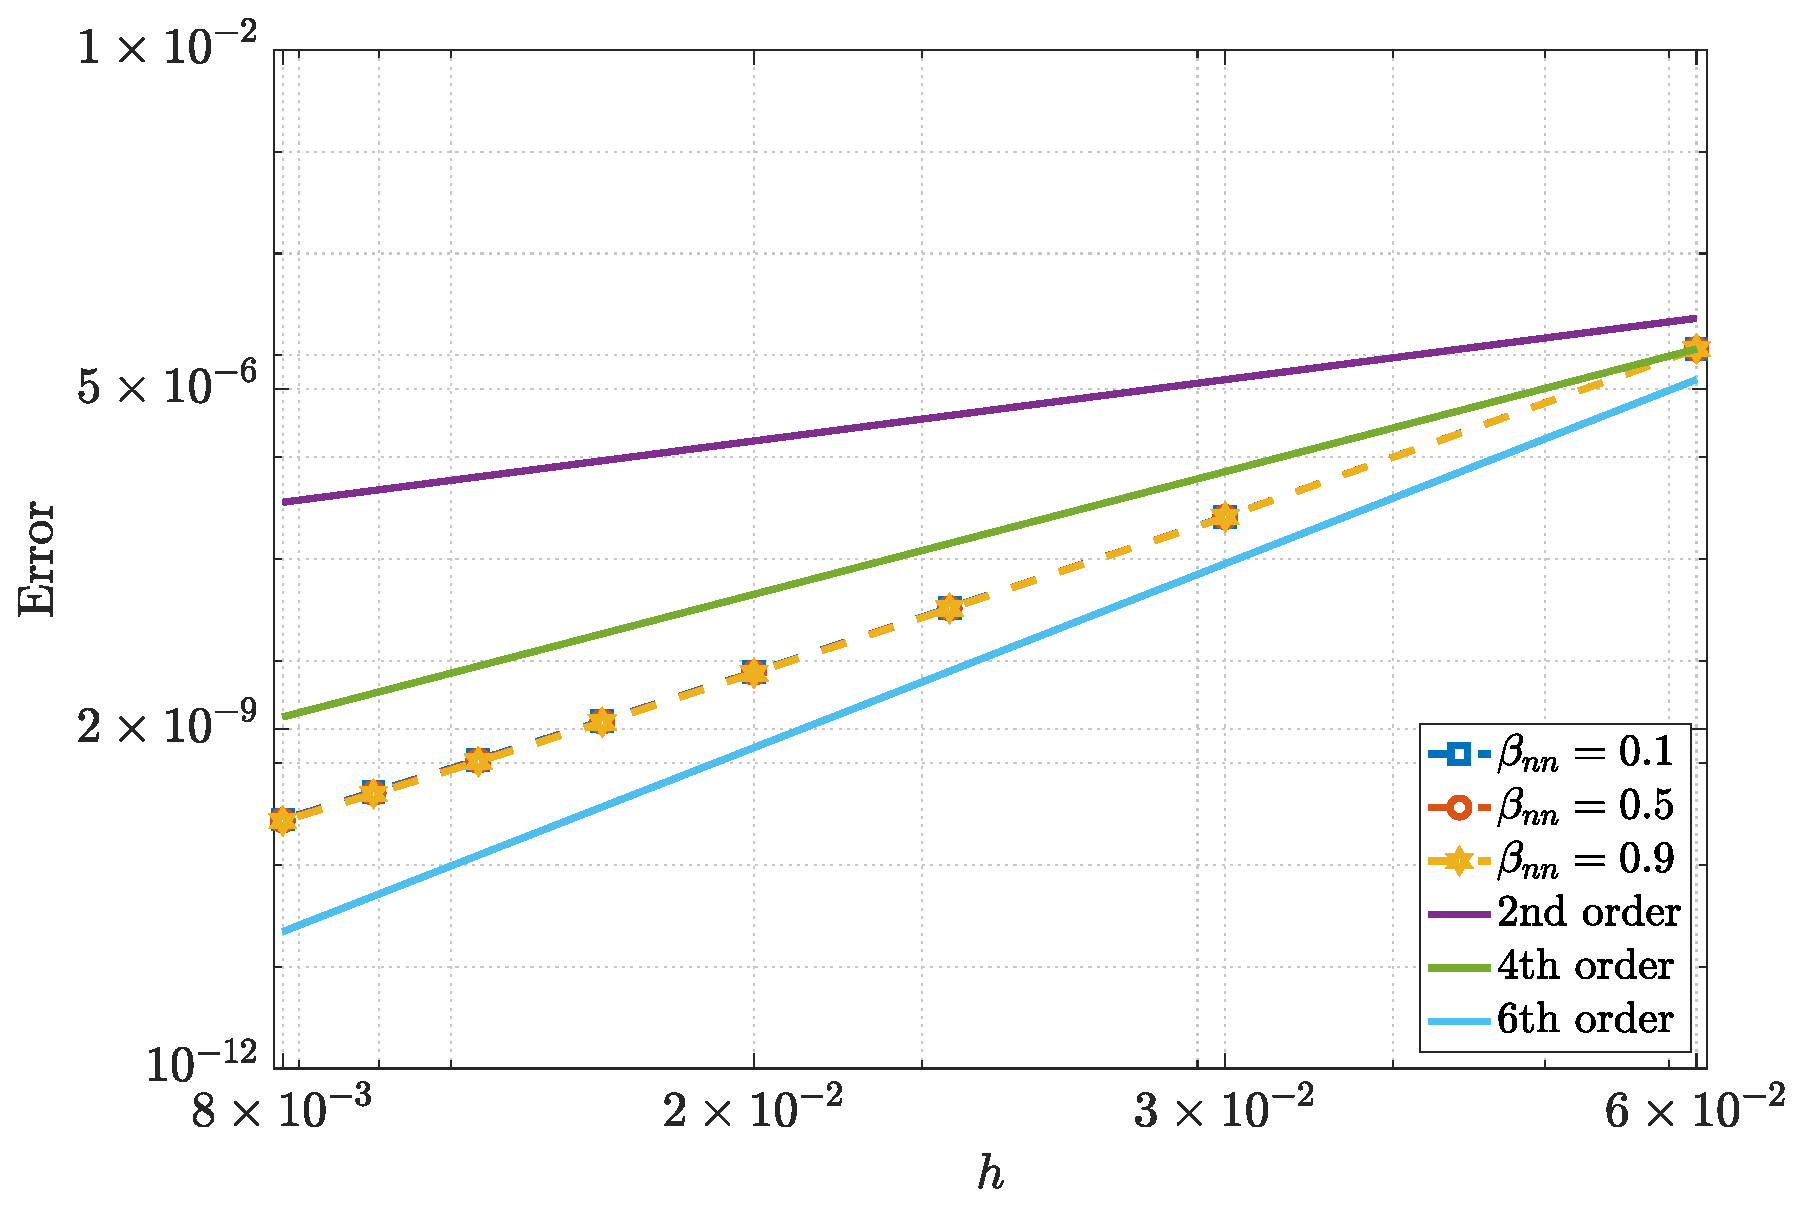
\includegraphics[width=\textwidth]{Figures/NormErr_2nd_Re_100_Wi_1_epsilon_0_xi_0_alphaG_0.1_Dt_1e-06_at_0.05_tipsim_1_MMS_12_Psi.eps}
        \captionof{subfigure}{$\tilde{\psi}$}
        \label{giesekus_psi_Case11}
    \end{minipage}
\end{frame}

%%%%%%%%%%%%%%%%%%%%%%%%%%%%%%%%%%%%%%%%%%%%%%%%%%%%%%%%%%%%%%
\begin{frame}{Caso de verificação usando o modelo Giesekus}
    \centering
    \captionsetup{justification=centering}
    \captionof{figure}{Erro para as componentes dos tensores de tensões, utilizando $Re=100$, $Wi=1$ e $\alpha_G=0.1$ para o escoamento de fluido viscoelástico como o modelo Giesekus}
    \label{fig:giesekus_3}
    \begin{minipage}{0.325\textwidth}
        \centering
        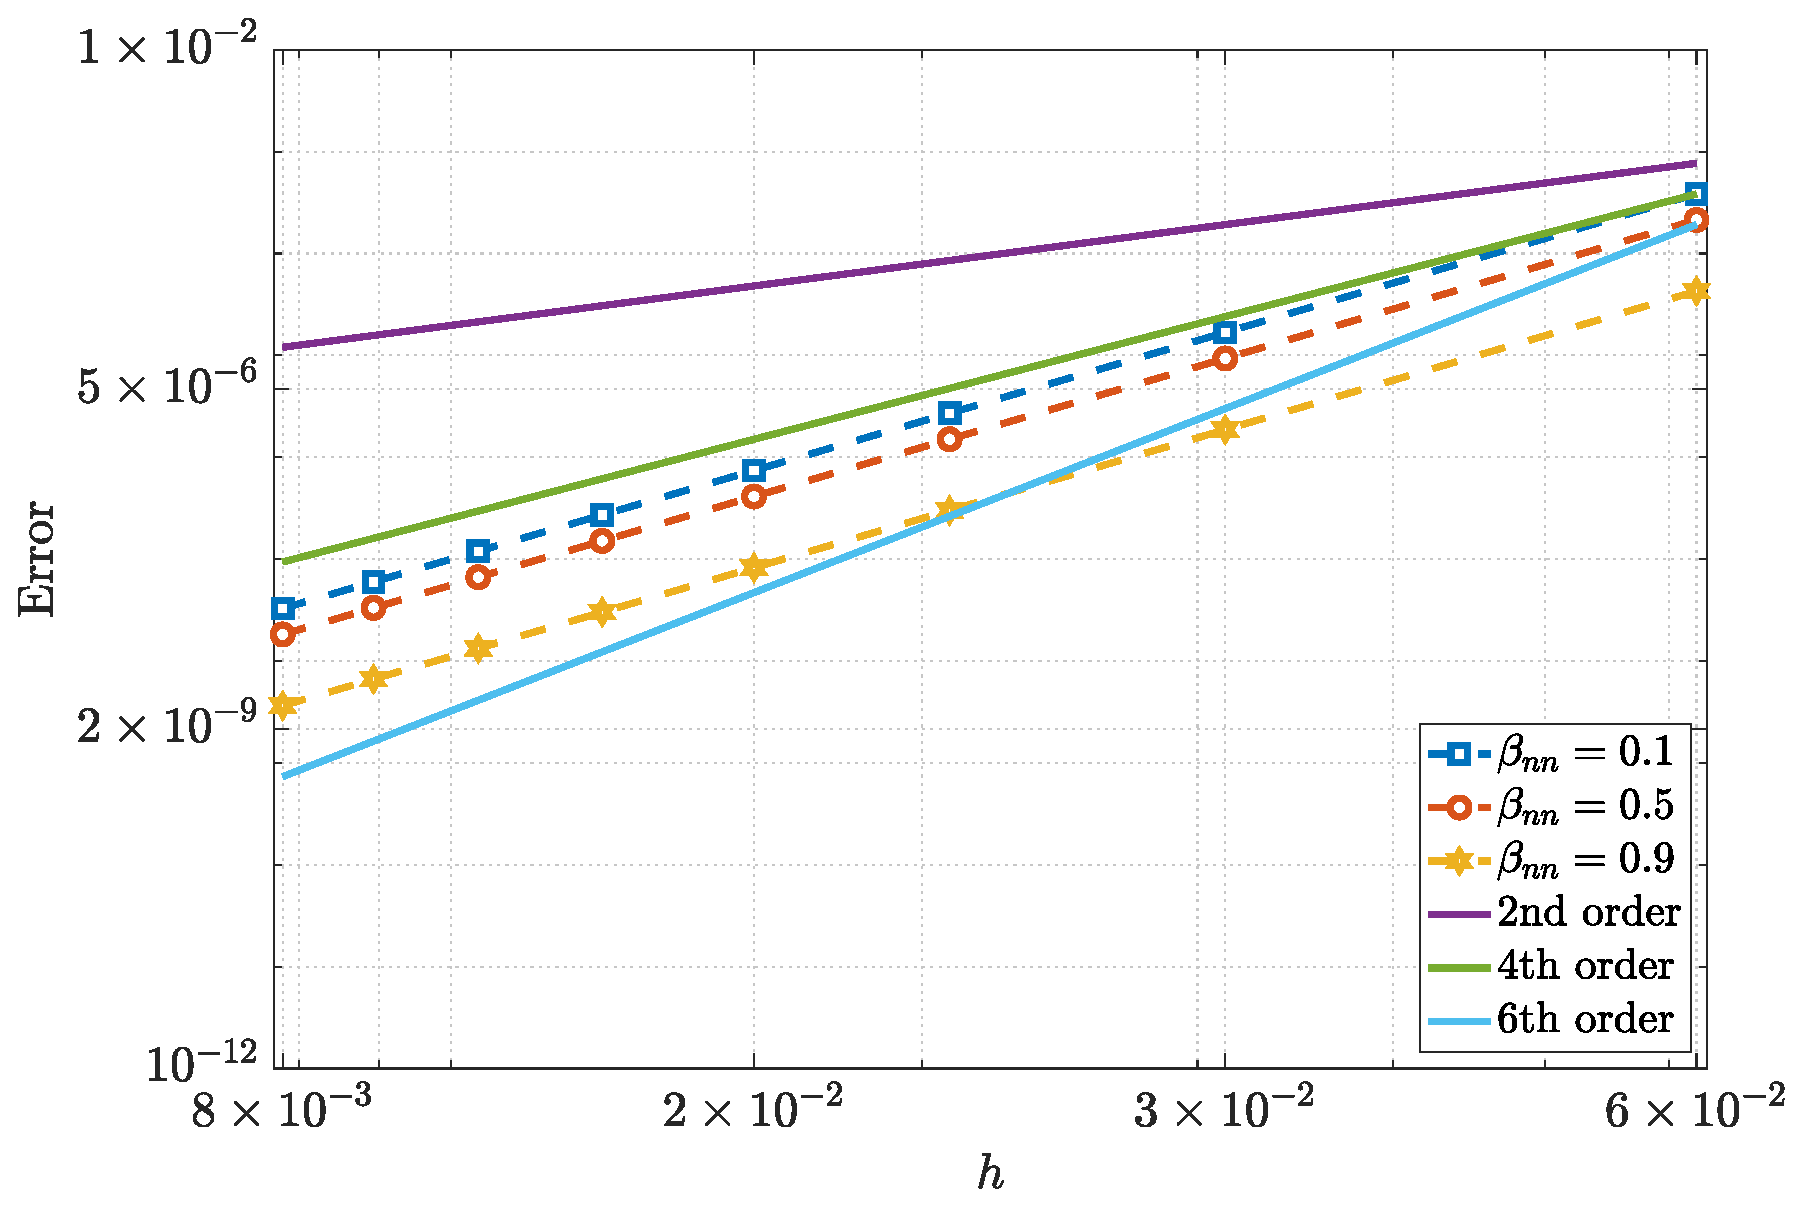
\includegraphics[width=\textwidth]{Figures/NormErr_2nd_Re_100_Wi_1_epsilon_0_xi_0_alphaG_0.1_Dt_1e-06_at_0.05_tipsim_1_MMS_12_Txx.eps}
        \captionof{subfigure}{$\overline{T_{xx}}$}
        \label{giesekus_txx_Case11}
    \end{minipage}
    \hfill
    \begin{minipage}{0.325\textwidth}
        \centering
        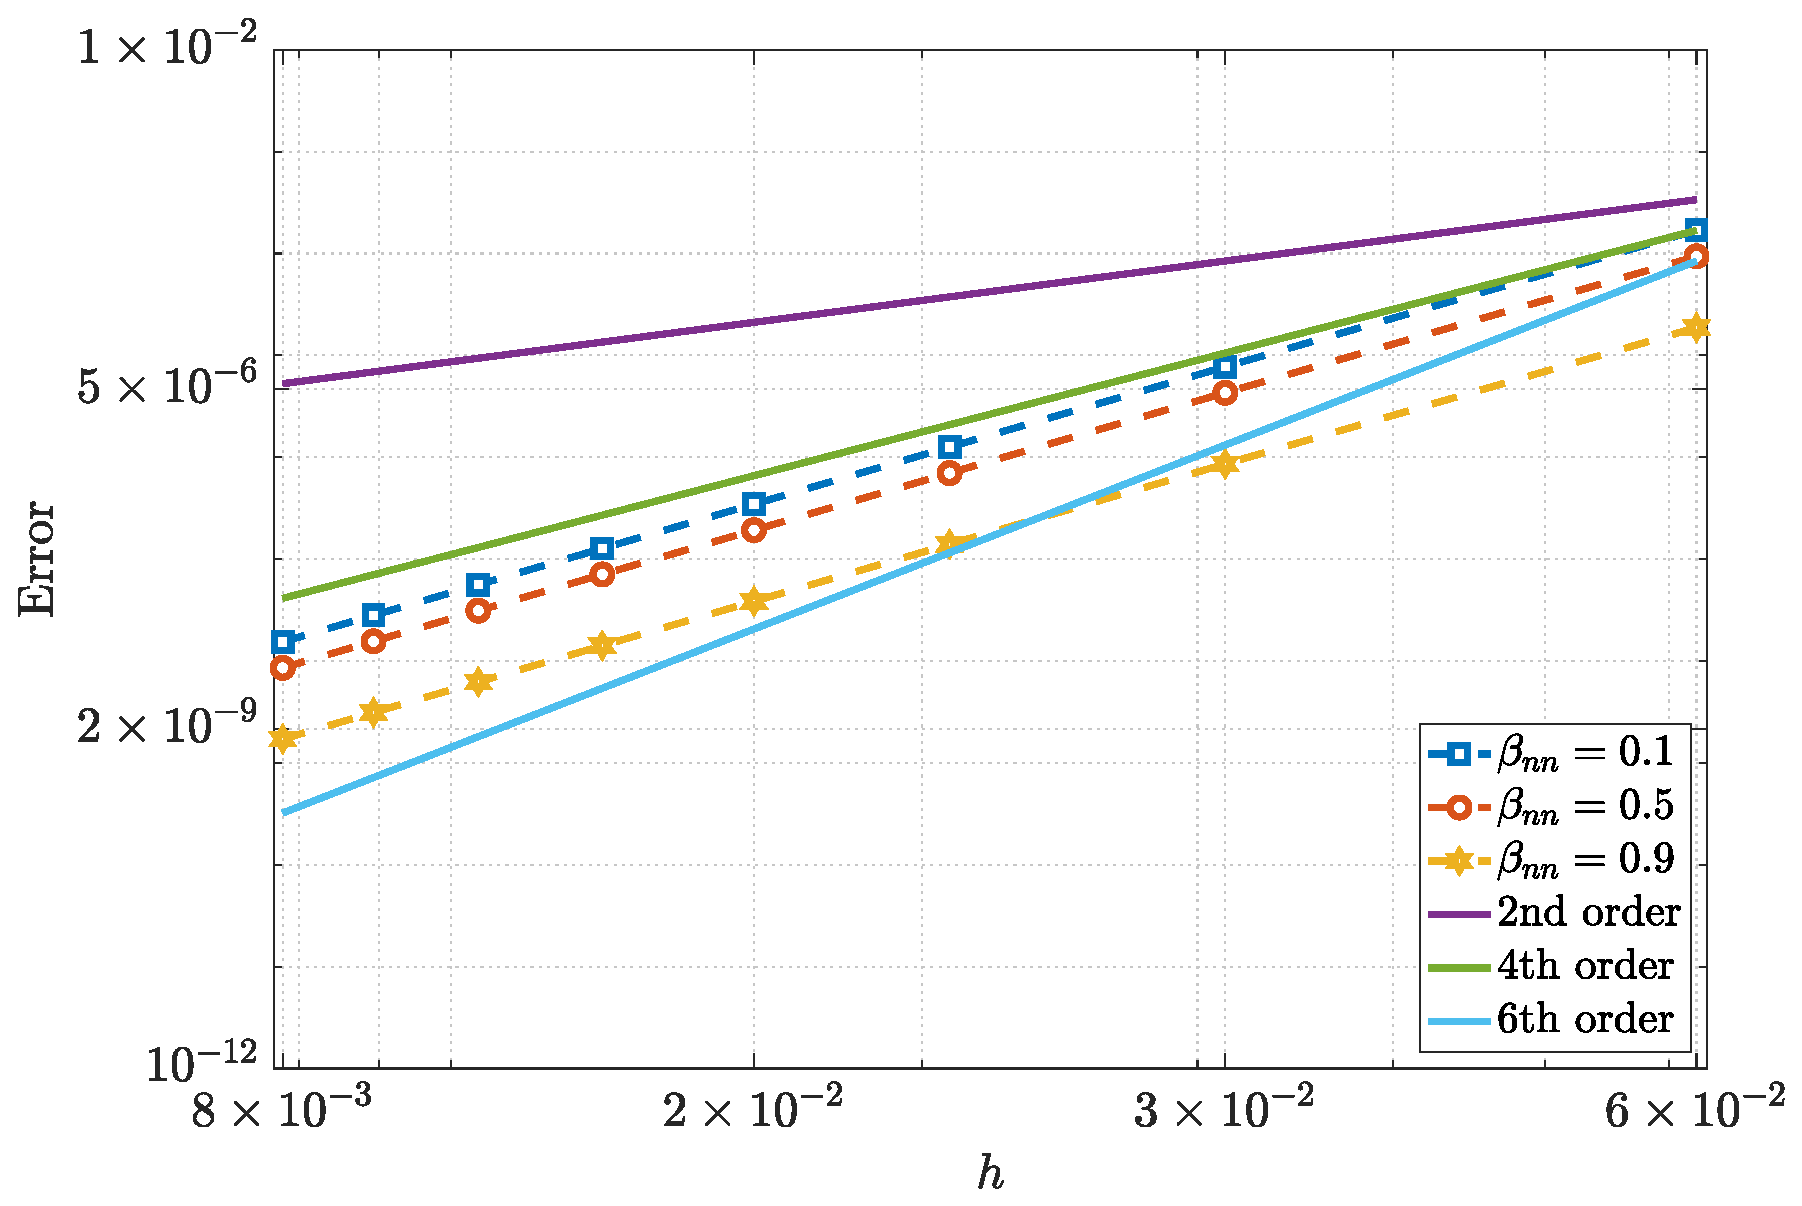
\includegraphics[width=\textwidth]{Figures/NormErr_2nd_Re_100_Wi_1_epsilon_0_xi_0_alphaG_0.1_Dt_1e-06_at_0.05_tipsim_1_MMS_12_Txy.eps}
        \captionof{subfigure}{$\overline{T_{xy}}$}
        \label{giesekus_txy_Case11}
    \end{minipage}
    \hfill
    \begin{minipage}{0.325\textwidth}
        \centering
        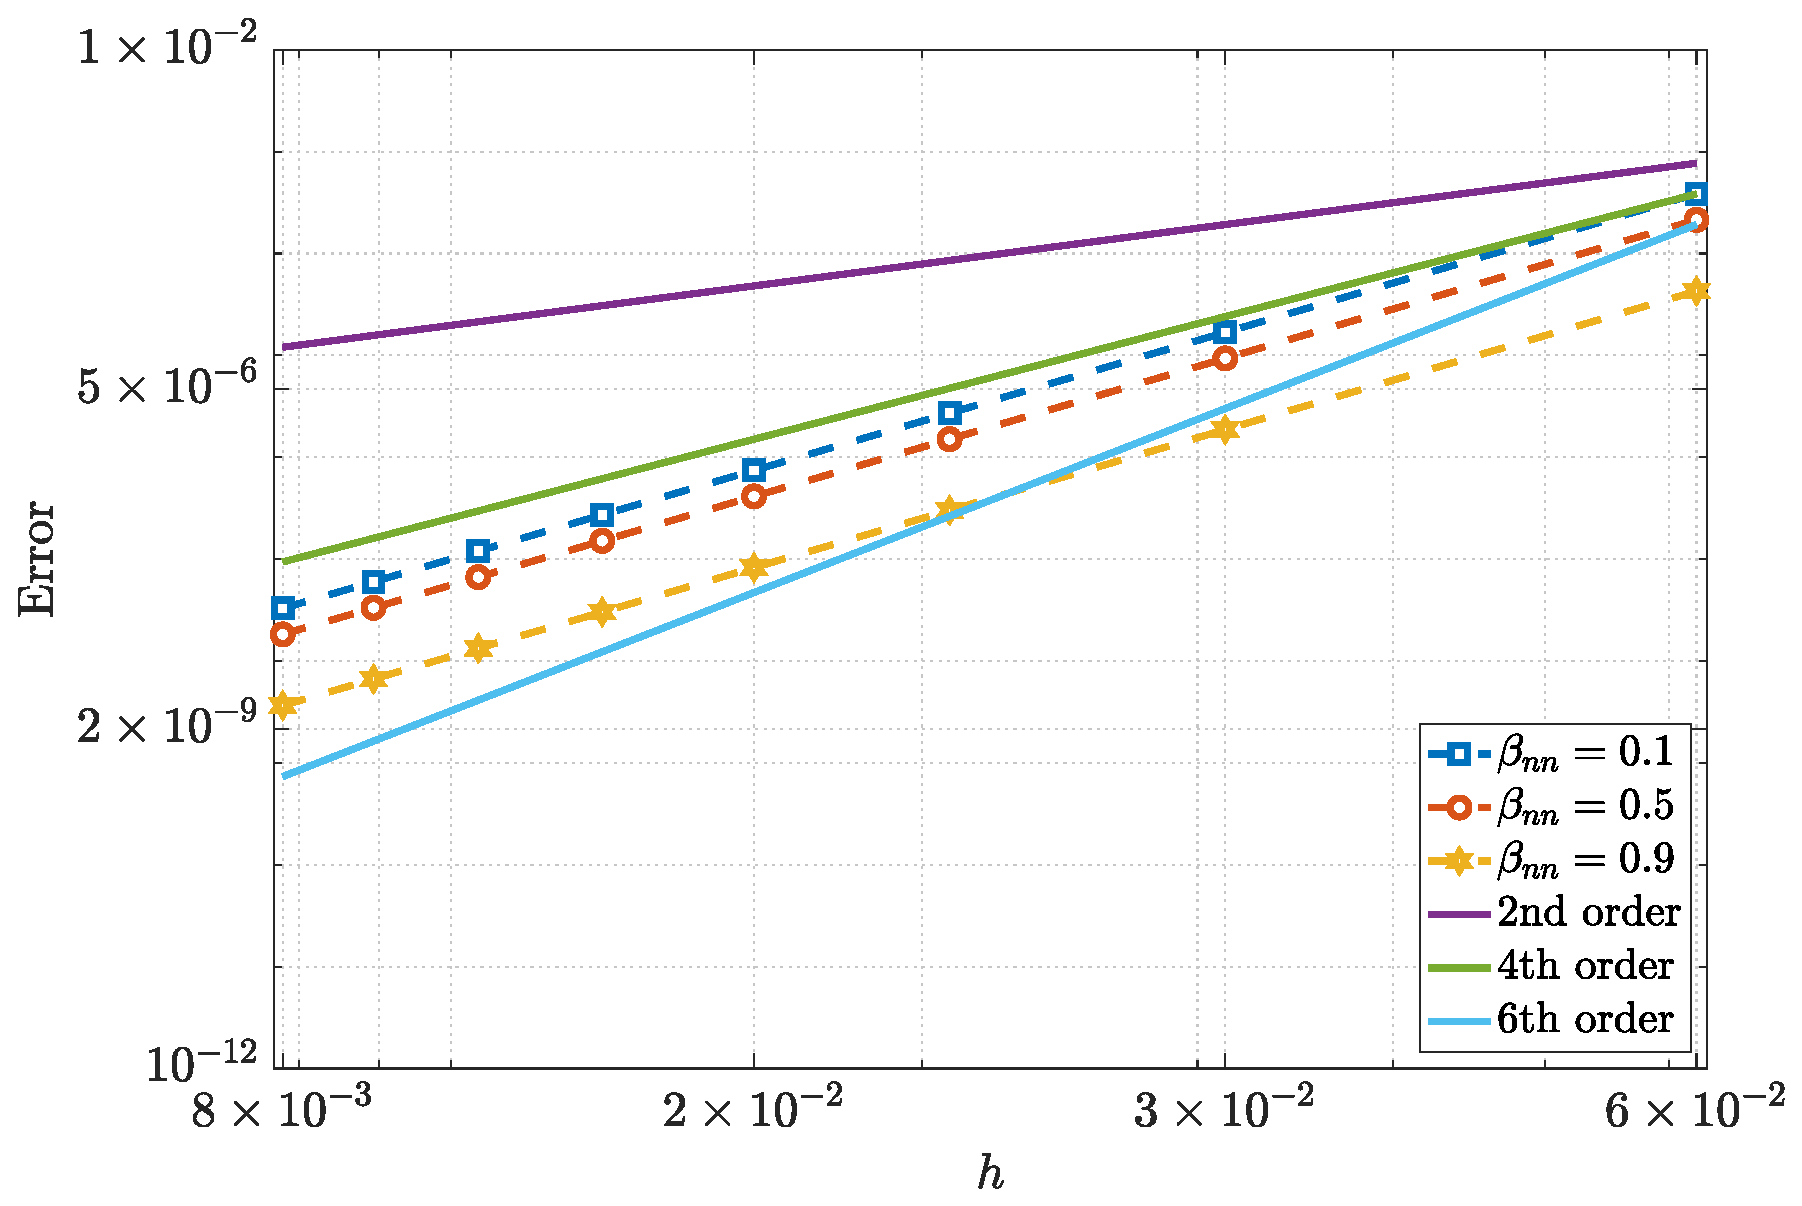
\includegraphics[width=\textwidth]{Figures/NormErr_2nd_Re_100_Wi_1_epsilon_0_xi_0_alphaG_0.1_Dt_1e-06_at_0.05_tipsim_1_MMS_12_Tyy.eps}
        \captionof{subfigure}{$\overline{T_{yy}}$}
        \label{giesekus_tyy_Case11}
    \end{minipage}
\end{frame}

%%%%%%%%%%%%%%%%%%%%%%%%%%%%%%%%%%%%%%%%%%%%%%%%%%%%%%%%%%%%%%
\begin{frame}{Caso de verificação usando o modelo LPTT}
    \centering
    \begin{table}[H]
\caption{Erros numéricos e cálculo da ordem de convergência para a vorticidade $(\omega_{z})$, utilizando o parâmetro $Wi=1$, para o escoamento de fluido viscoelástico LPTT.\label{tab_LPTTWzResumida_2}}
\scriptsize{
    \begin{tabular*}{\textwidth}{@{\extracolsep\fill}cccccccccc@{}}
    \hline
    \multirow{2}{*}{$\operatorname{Re}$} & \multirow{2}{*}{Malha} & \multicolumn{2}{c}{$\beta_{nn}=0.1$}  & \multicolumn{2}{c}{$\beta_{nn}=0.5$}  & \multicolumn{2}{c}{$\beta_{nn}=0.9$}  & \multicolumn{2}{c}{$\beta_{nn}=1.0$}\\ %\cline{2-10}
     & & Erro & Ordem & Erro & Ordem & Erro & Ordem & Erro & Ordem \\
    \hline
    \multirow{10}{*}{1.00} & $17\times 17$ & 3.02e-03 & --- & 2.77e-03 & --- & 2.57e-03 & --- & 2.52e-03 & --- \\
    & $33\times 33$ & 2.54e-04 & 3.57 & 1.70e-04 & 4.03 & 1.35e-04 & 4.25 & 1.29e-04 & 4.29 \\
    & $49\times 49$ & 4.87e-05 & 4.07 & 2.59e-05 & 4.64 & 1.99e-05 & 4.72 & 1.90e-05 & 4.73 \\
    & $65\times 65$ & 1.32e-05 & 4.53 & 6.41e-06 & 4.85 & 4.91e-06 & 4.86 & 4.68e-06 & 4.86 \\
    & $81\times 81$ & 4.46e-06 & 4.87 & 2.14e-06 & 4.91 & 1.67e-06 & 4.84 & 1.60e-06 & 4.81 \\
    & $97\times 97$ & 1.76e-06 & 5.09 & 8.69e-07 & 4.95 & 6.98e-07 & 4.77 & 6.76e-07 & 4.72 \\
    & $113\times 133$ & 7.91e-07 & 5.20 & 4.11e-07 & 4.86 & 3.46e-07 & 4.55 & 3.38e-07 & 4.50 \\
    & $129\times 129$ & 4.07e-07 & 4.98 & 2.39e-07 & 4.05 & 2.14e-07 & 3.61 & 2.11e-07 & 3.54 \\
    \hline
    \multirow{10}{*}{100.00} & $17\times 17$ & 3.10e-03 & --- & 3.09e-03 & --- & 3.08e-03 & --- & 3.08e-03 & --- \\
    & $33\times 33$ & 2.93e-04 & 3.40 & 2.91e-04 & 3.41 & 2.88e-04 & 3.42 & 2.88e-04 & 3.42 \\
    & $49\times 49$ & 6.76e-05 & 3.62 & 6.65e-05 & 3.64 & 6.54e-05 & 3.66 & 6.51e-05 & 3.66 \\
    & $65\times 65$ & 2.30e-05 & 3.75 & 2.23e-05 & 3.79 & 2.17e-05 & 3.83 & 2.16e-05 & 3.84 \\
    & $81\times 81$ & 9.72e-06 & 3.86 & 9.28e-06 & 3.93 & 8.88e-06 & 4.01 & 8.79e-06 & 4.02 \\
    & $97\times 97$ & 4.66e-06 & 4.03 & 4.36e-06 & 4.14 & 4.09e-06 & 4.25 & 4.03e-06 & 4.27 \\
    & $113\times 133$ & 2.42e-06 & 4.25 & 2.21e-06 & 4.41 & 2.03e-06 & 4.55 & 1.99e-06 & 4.58 \\
    & $129\times 129$ & 1.38e-06 & 4.22 & 1.22e-06 & 4.46 & 1.09e-06 & 4.67 & 1.06e-06 & 4.71 \\
    \hline
    \end{tabular*}
}
\end{table}
\end{frame}


%%%%%%%%%%%%%%%%%%%%%%%%%%%%%%%%%%%%%%%%%%%%%%%%%%%%%%%%%%%%%%
\begin{frame}{Caso de verificação usando o modelo LPTT}
    \centering
    \begin{table}[H]
\caption{Erros numéricos e cálculo da ordem de convergência para a vorticidade $(\omega_{z})$, utilizando o parâmetro $Wi=1$, para o escoamento de fluido viscoelástico LPTT.\label{tab_LPTTWzResumida_1}}
\scriptsize{
    \begin{tabular*}{\textwidth}{@{\extracolsep\fill}cccccccccc@{}}
    \hline
    \multirow{2}{*}{$\operatorname{Re}$} & \multirow{2}{*}{Malha} & \multicolumn{2}{c}{$\beta_{nn}=0.1$}  & \multicolumn{2}{c}{$\beta_{nn}=0.5$}  & \multicolumn{2}{c}{$\beta_{nn}=0.9$}  & \multicolumn{2}{c}{$\beta_{nn}=1.0$}\\ %\cline{2-10}
     & & Erro & Ordem & Erro & Ordem & Erro & Ordem & Erro & Ordem \\
    \hline
    \multirow{10}{*}{400.00} & $17\times 17$ & 3.10e-03 & --- & 3.09e-03 & --- & 3.08e-03 & --- & 3.08e-03 & --- \\
    & $33\times 33$ & 2.93e-04 & 3.40 & 2.92e-04 & 3.40 & 2.91e-04 & 3.40 & 2.91e-04 & 3.40 \\
    & $49\times 49$ & 6.78e-05 & 3.61 & 6.74e-05 & 3.62 & 6.71e-05 & 3.62 & 6.70e-05 & 3.62 \\
    & $65\times 65$ & 2.31e-05 & 3.74 & 2.29e-05 & 3.75 & 2.28e-05 & 3.76 & 2.27e-05 & 3.76 \\
    & $81\times 81$ & 9.81e-06 & 3.84 & 9.69e-06 & 3.86 & 9.58e-06 & 3.88 & 9.55e-06 & 3.88 \\
    & $97\times 97$ & 4.72e-06 & 4.01 & 4.64e-06 & 4.03 & 4.57e-06 & 4.06 & 4.55e-06 & 4.06 \\
    & $113\times 133$ & 2.47e-06 & 4.21 & 2.41e-06 & 4.25 & 2.36e-06 & 4.28 & 2.35e-06 & 4.29 \\
    & $129\times 129$ & 1.42e-06 & 4.16 & 1.37e-06 & 4.22 & 1.33e-06 & 4.27 & 1.33e-06 & 4.28 \\
    \hline
    \multirow{10}{*}{1000.00} & $17\times 17$ & 3.10e-03 & --- & 3.09e-03 & --- & 3.09e-03 & --- & 3.08e-03 & --- \\
    & $33\times 33$ & 2.93e-04 & 3.40 & 2.93e-04 & 3.40 & 2.92e-04 & 3.40 & 2.92e-04 & 3.40 \\
    & $49\times 49$ & 6.78e-05 & 3.61 & 6.76e-05 & 3.61 & 6.74e-05 & 3.61 & 6.74e-05 & 3.61 \\
    & $65\times 65$ & 2.32e-05 & 3.73 & 2.31e-05 & 3.74 & 2.30e-05 & 3.74 & 2.30e-05 & 3.74 \\
    & $81\times 81$ & 9.84e-06 & 3.84 & 9.78e-06 & 3.85 & 9.73e-06 & 3.85 & 9.72e-06 & 3.85 \\
    & $97\times 97$ & 4.75e-06 & 4.00 & 4.71e-06 & 4.01 & 4.68e-06 & 4.02 & 4.67e-06 & 4.02 \\
    & $113\times 133$ & 2.49e-06 & 4.19 & 2.46e-06 & 4.21 & 2.44e-06 & 4.23 & 2.43e-06 & 4.23 \\
    & $129\times 129$ & 1.43e-06 & 4.13 & 1.41e-06 & 4.16 & 1.39e-06 & 4.18 & 1.39e-06 & 4.18 \\
    \hline
    \end{tabular*}
}
\end{table}
\end{frame}

%%%%%%%%%%%%%%%%%%%%%%%%%%%%%%%%%%%%%%%%%%%%%%%%%%%%%%%%%%%%%%
\begin{frame}{Caso de verificação usando o modelo LPTT}
    \centering
    \captionsetup{justification=centering}
    \captionof{figure}{Erro para o campo de velocidades $(\overline{u},\tilde{v})$ utilizando $Re=100$, $Wi=1$, $\epsilon = 0.5$ e $\xi = 0.1$ para o escoamento de fluido viscoelástico como o modelo LPTT}
    \label{fig:lptt_1}
    \begin{minipage}{0.49\textwidth}
        \centering
        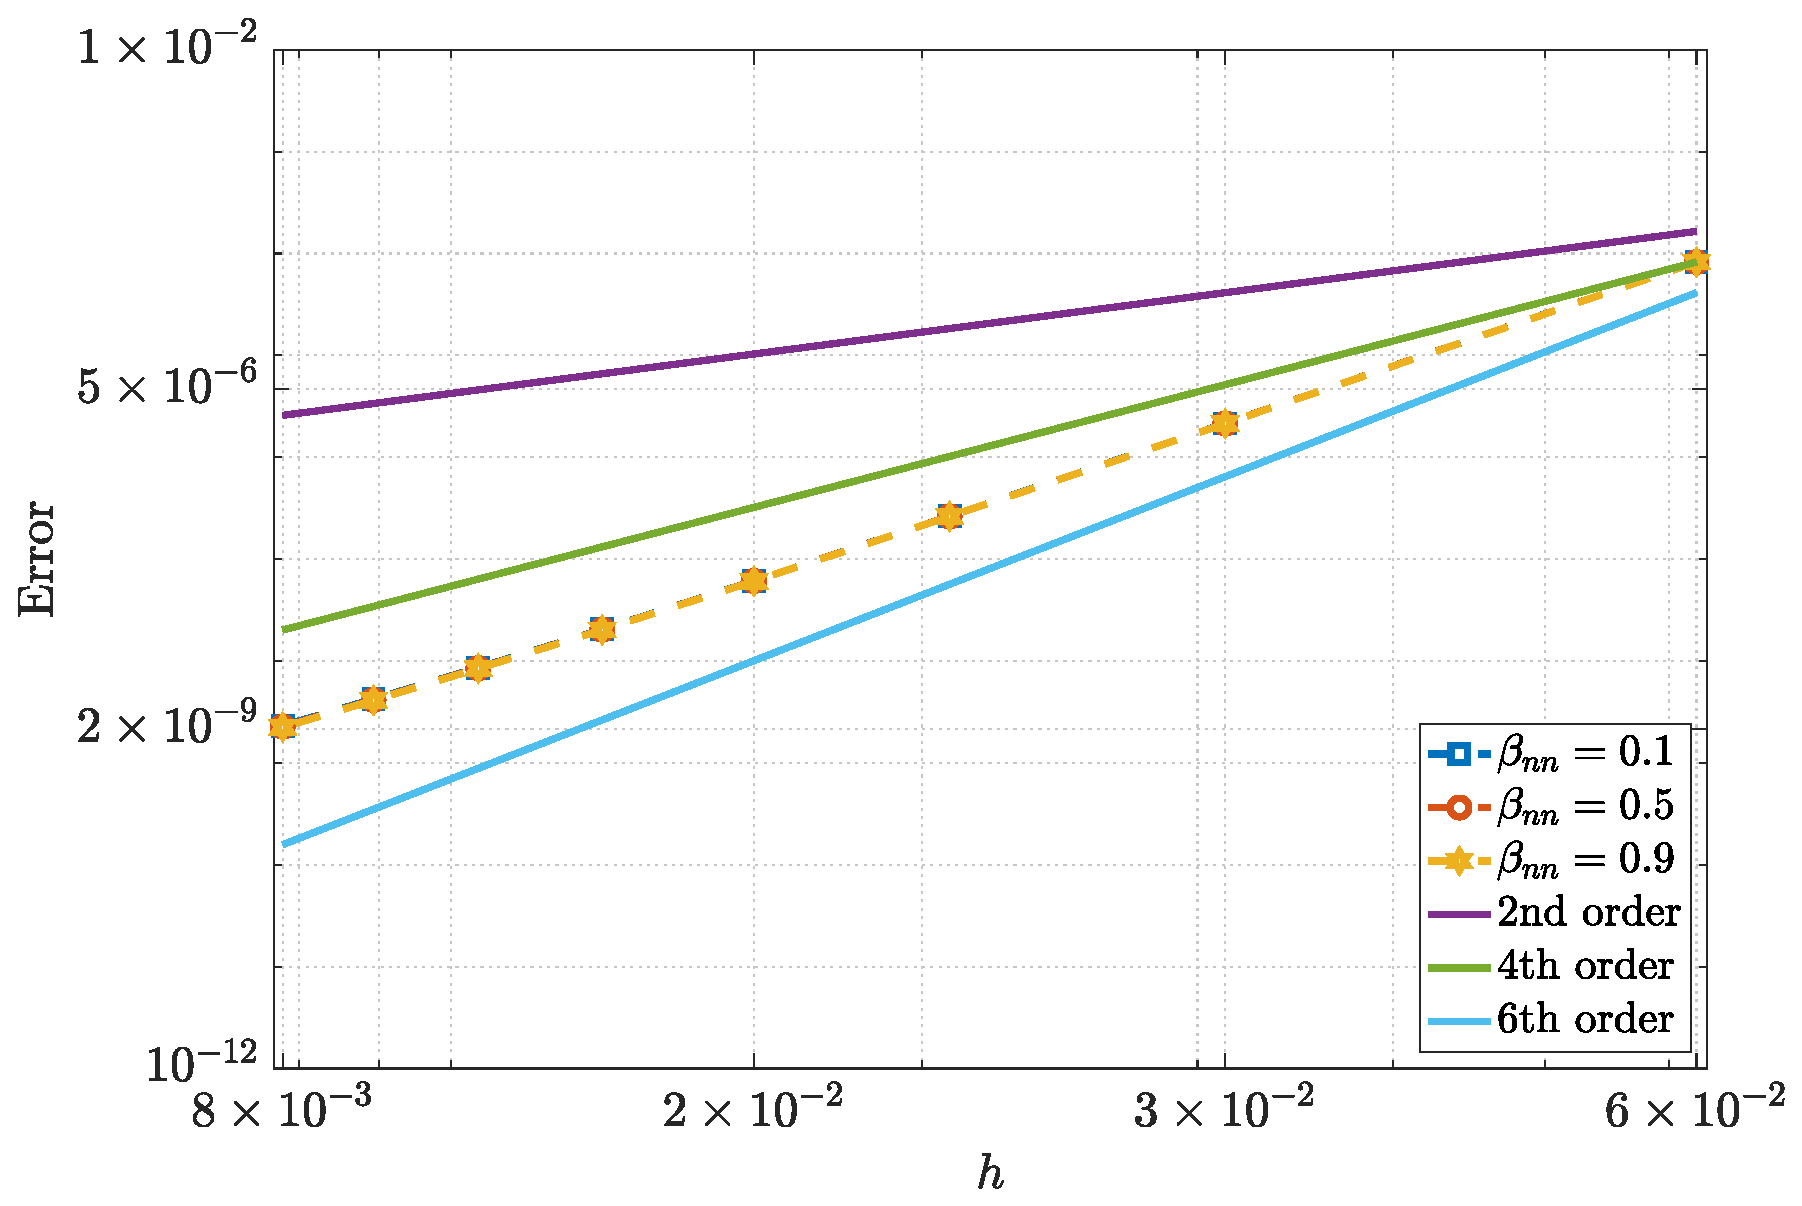
\includegraphics[width=\textwidth]{Figures/NormErr_2nd_Re_100_Wi_1_epsilon_0_xi_0_alphaG_0_Dt_1e-06_at_0.05_tipsim_1_MMS_12_U.eps}
        \captionof{subfigure}{$\overline{u}$}
        \label{lptt_u_Case11}
    \end{minipage}
    \hfill
    \begin{minipage}{0.49\textwidth}
        \centering
        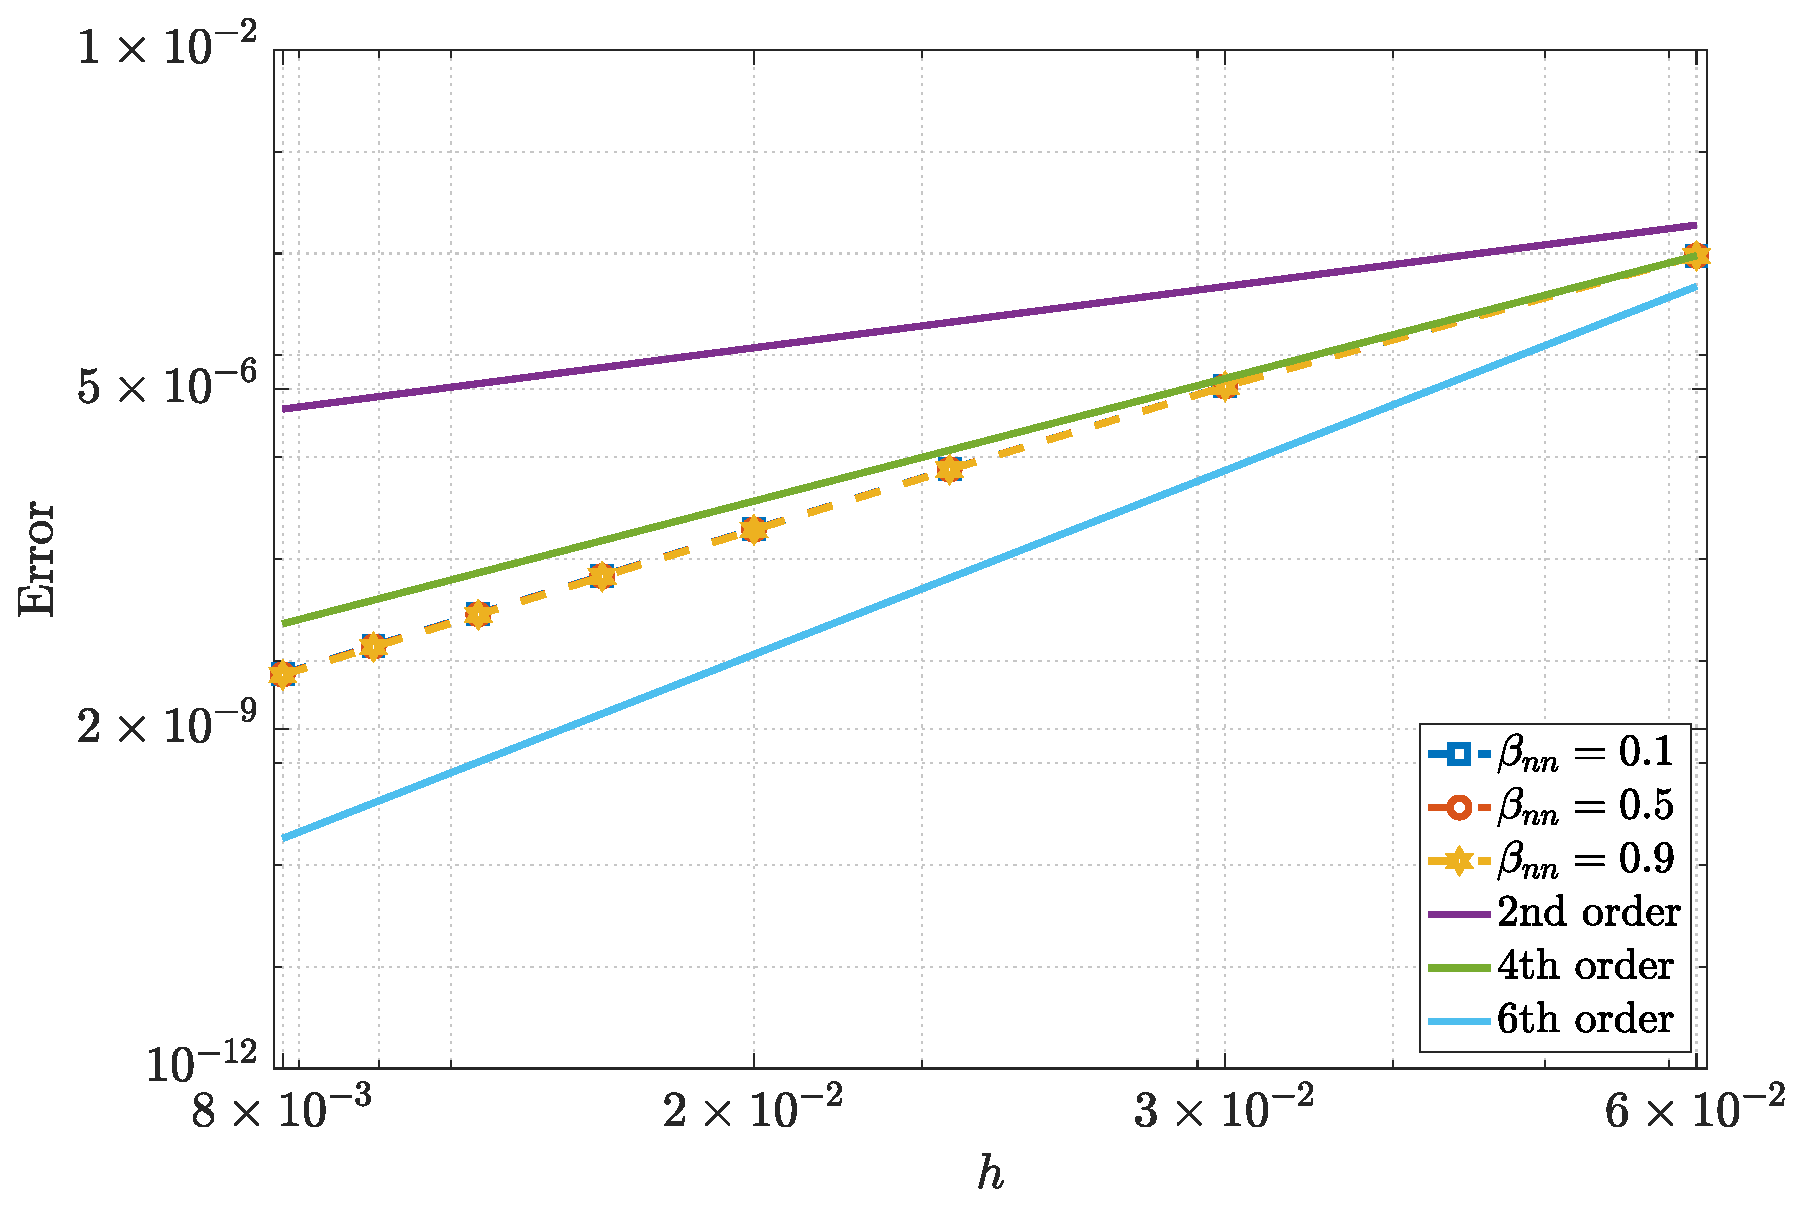
\includegraphics[width=\textwidth]{Figures/NormErr_2nd_Re_100_Wi_1_epsilon_0_xi_0_alphaG_0_Dt_1e-06_at_0.05_tipsim_1_MMS_12_V.eps}
        \captionof{subfigure}{$\tilde{v}$}
        \label{lptt_v_Case11}
    \end{minipage}
\end{frame}

%%%%%%%%%%%%%%%%%%%%%%%%%%%%%%%%%%%%%%%%%%%%%%%%%%%%%%%%%%%%%%
\begin{frame}{Caso de verificação usando o modelo LPTT}
    \centering
    \captionsetup{justification=centering}
    \captionof{figure}{Erro para a vorticidade $(\tilde{\omega_{z}})$ e função de corrente $(\tilde{\psi})$, utilizando $Re=100$, $Wi=1$, $\epsilon = 0.5$ e $\xi = 0.1$ para o escoamento de fluido viscoelástico como o modelo LPTT}
    \label{fig:lptt_2}
    \begin{minipage}{0.49\textwidth}
        \centering
        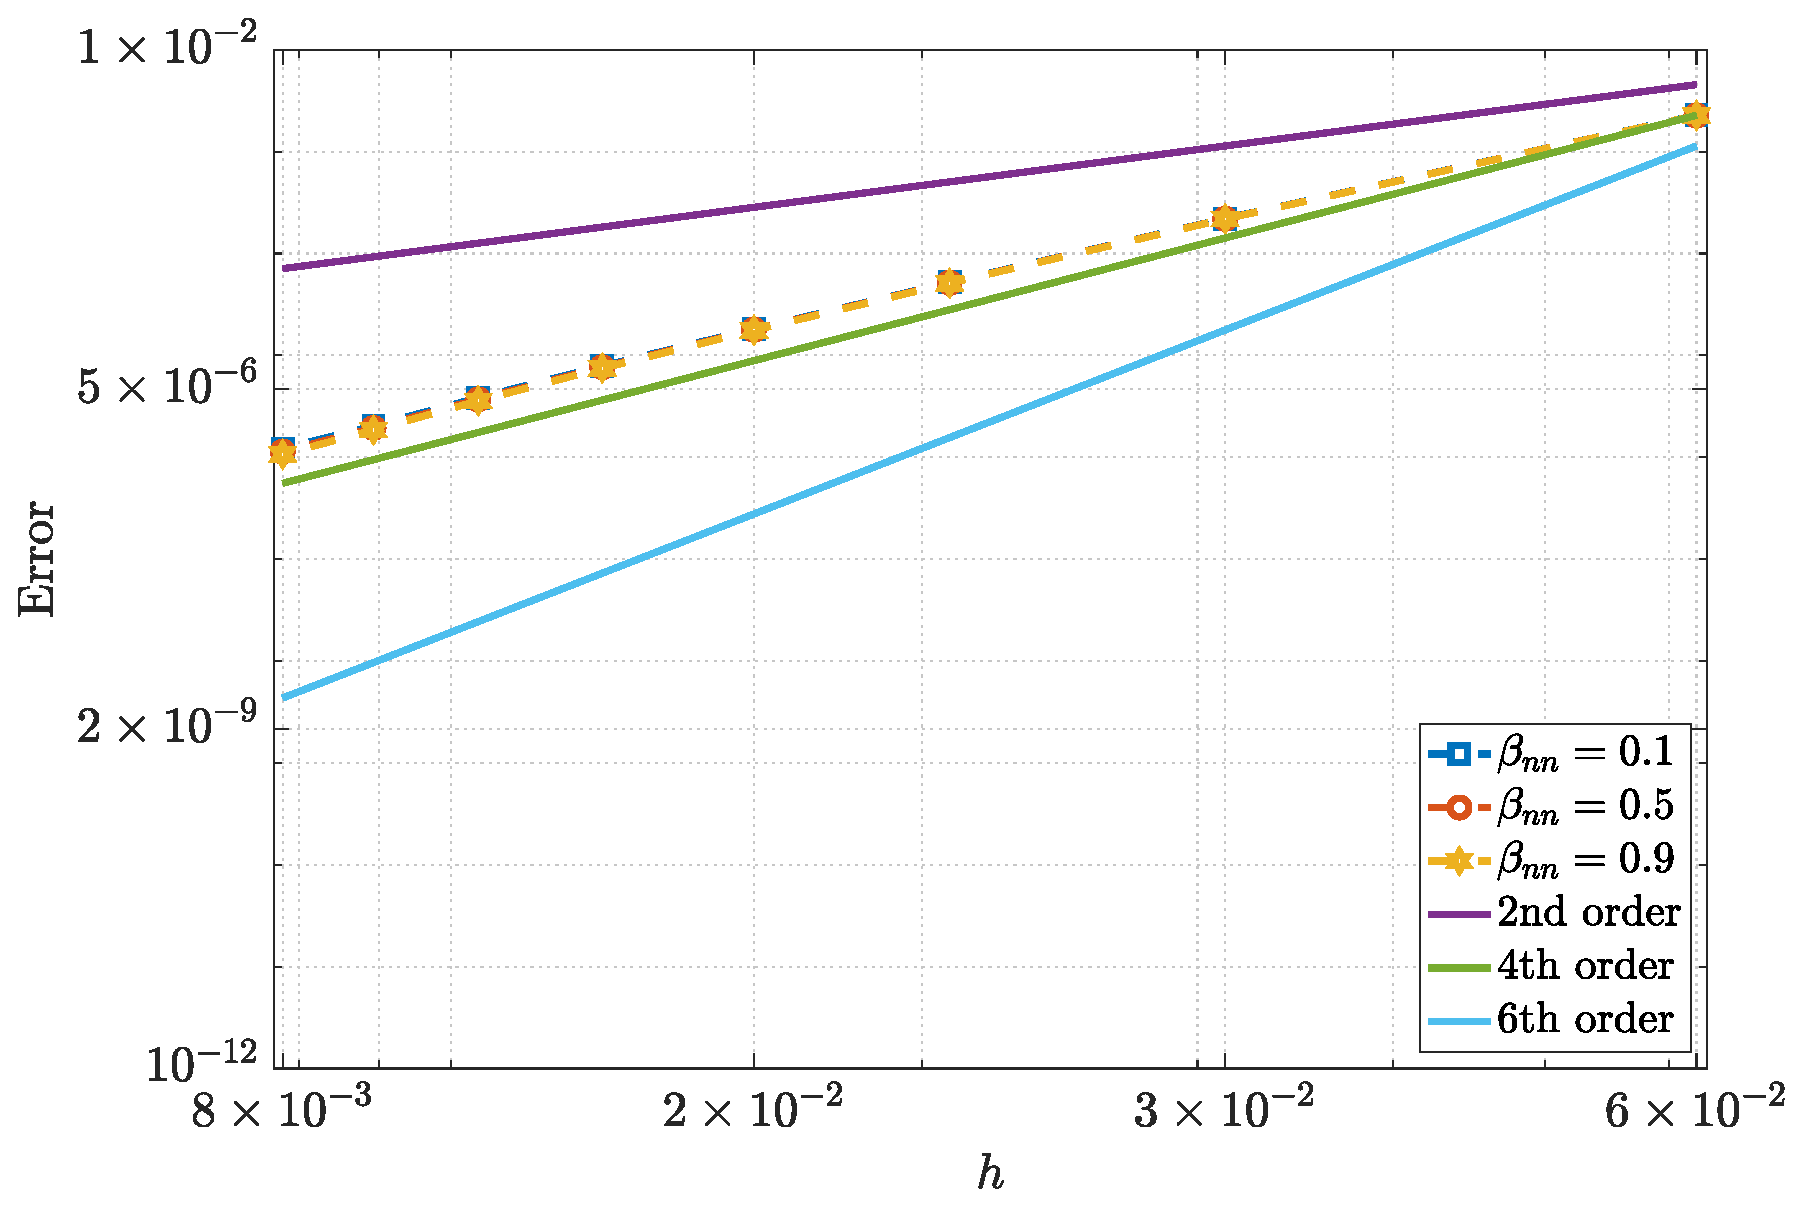
\includegraphics[width=\textwidth]{Figures/NormErr_2nd_Re_100_Wi_1_epsilon_0_xi_0_alphaG_0_Dt_1e-06_at_0.05_tipsim_1_MMS_12_Wz.eps}
        \captionof{subfigure}{$\tilde{\omega_{z}}$}
        \label{lptt_wz_Case11}
    \end{minipage}
    \hfill
    \begin{minipage}{0.49\textwidth}
        \centering
        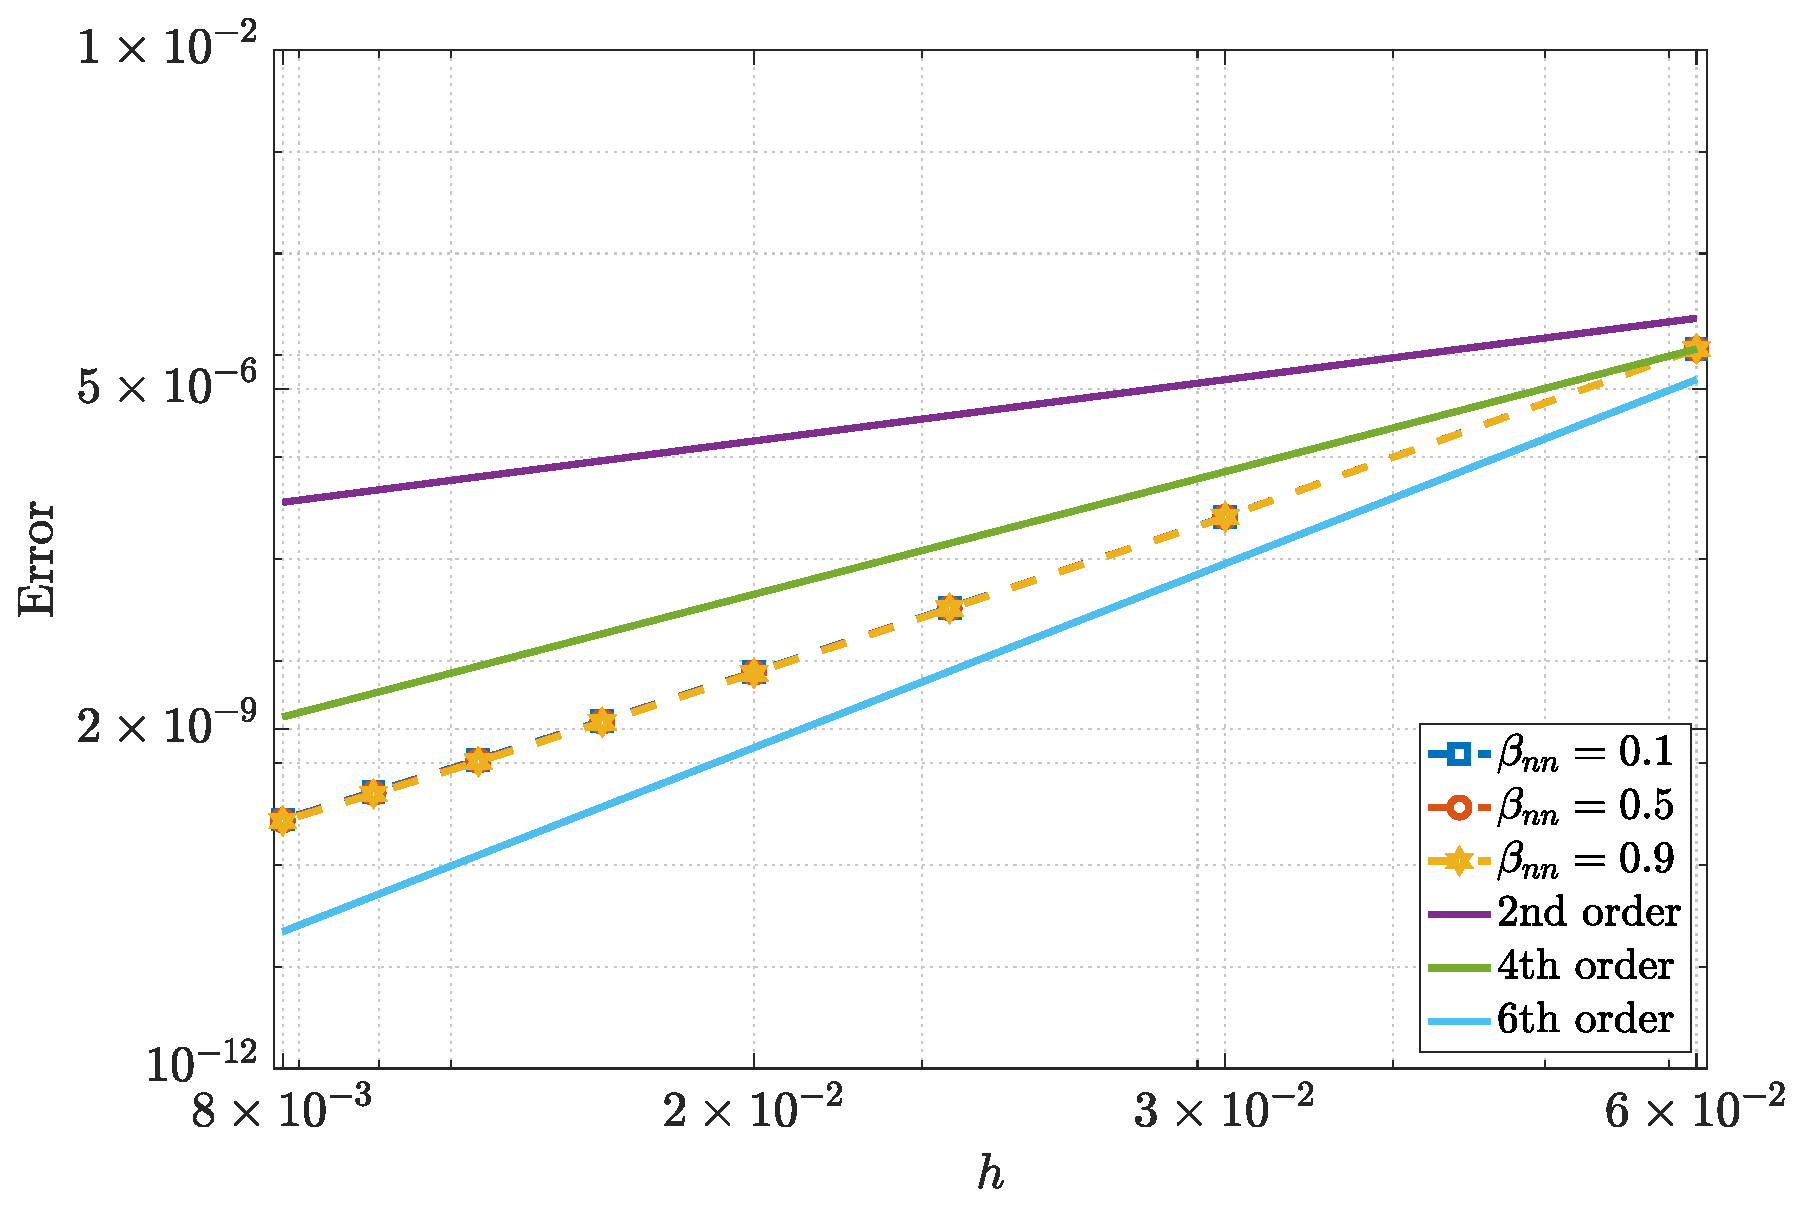
\includegraphics[width=\textwidth]{Figures/NormErr_2nd_Re_100_Wi_1_epsilon_0_xi_0_alphaG_0_Dt_1e-06_at_0.05_tipsim_1_MMS_12_Psi.eps}
        \captionof{subfigure}{$\tilde{\psi}$}
        \label{lptt_psi_Case11}
    \end{minipage}
\end{frame}

%%%%%%%%%%%%%%%%%%%%%%%%%%%%%%%%%%%%%%%%%%%%%%%%%%%%%%%%%%%%%%
\begin{frame}{Caso de verificação usando o modelo LPTT}
    \centering
    \captionsetup{justification=centering}
    \captionof{figure}{Erro para as componentes dos tensores de tensões, utilizando $Re=100$, $Wi=1$, $\epsilon = 0.5$ e $\xi = 0.1$ para o escoamento de fluido viscoelástico como o modelo LPTT}
    \label{fig:lptt_3}
    \begin{minipage}{0.325\textwidth}
        \centering
        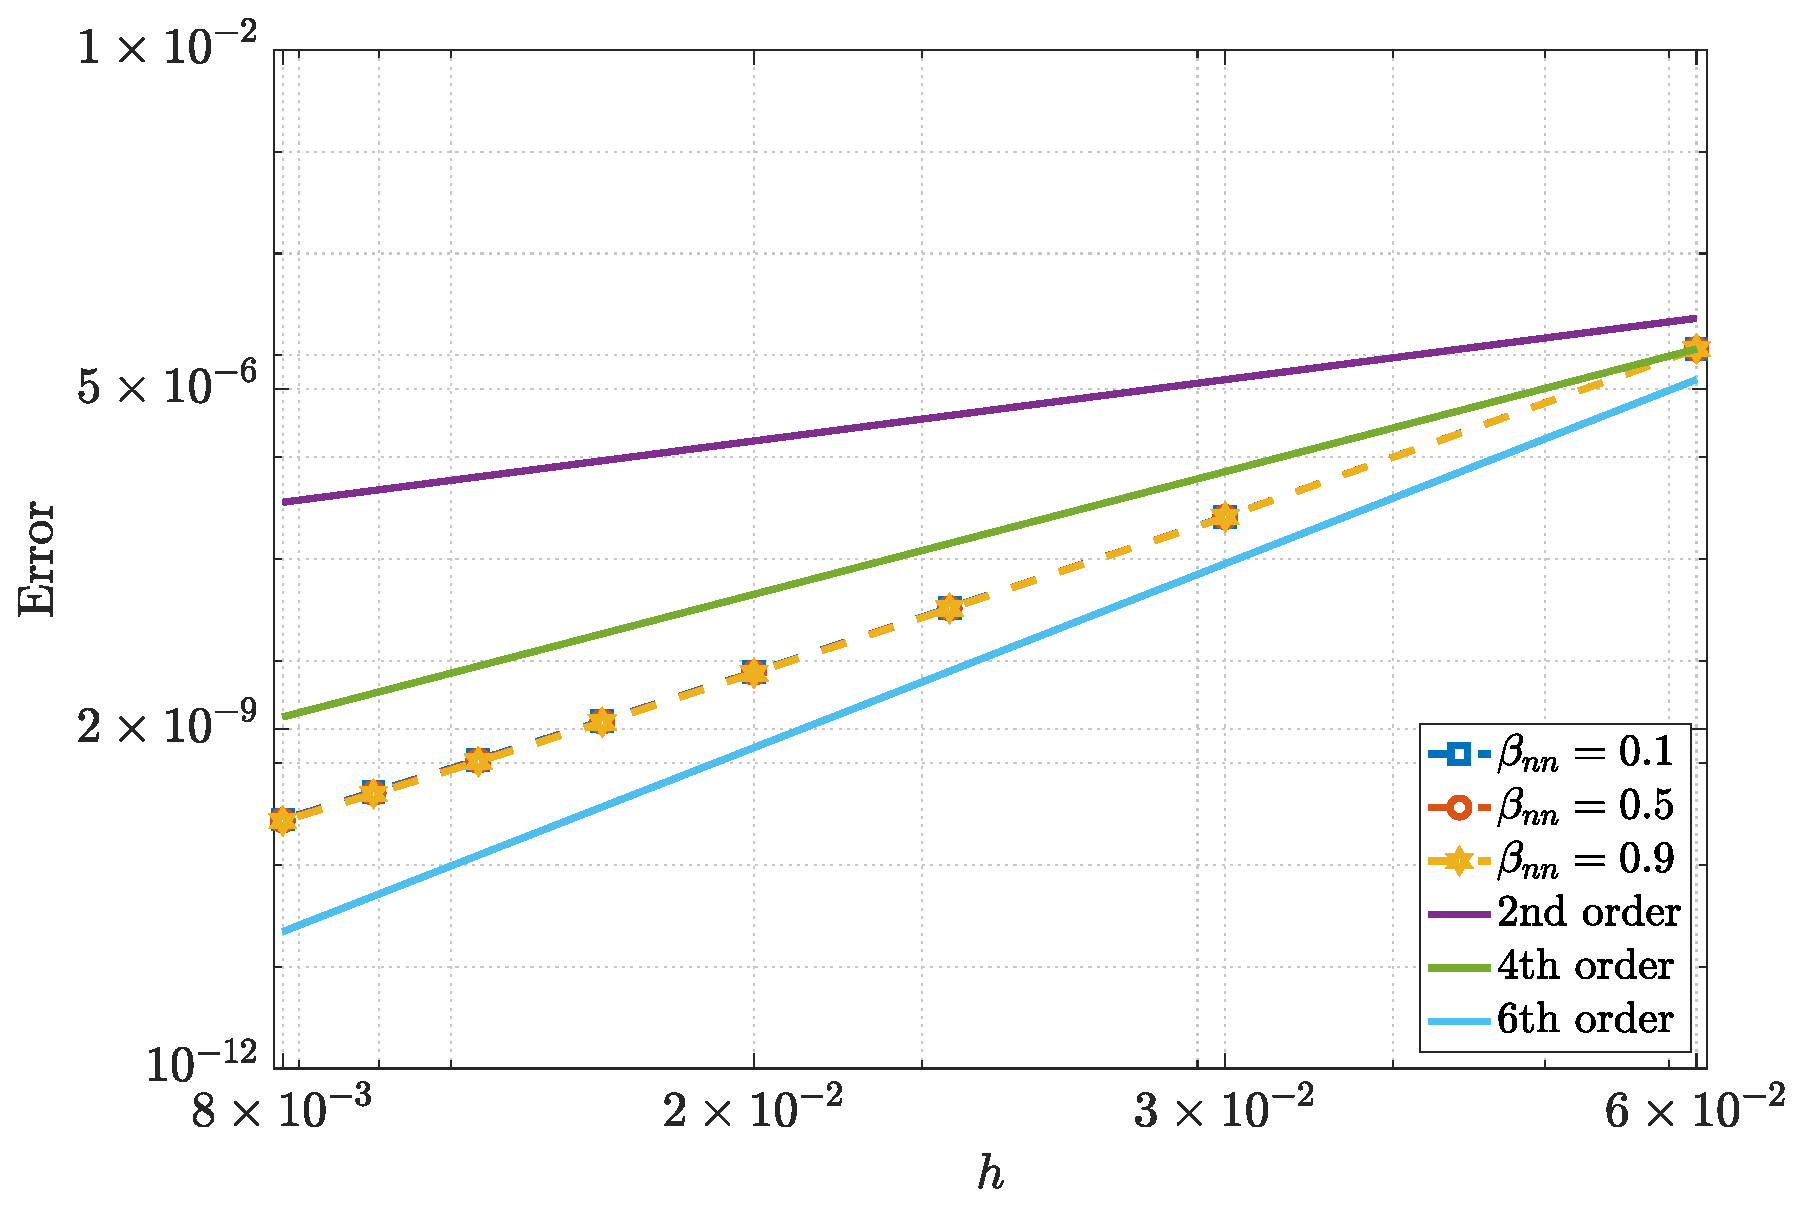
\includegraphics[width=\textwidth]{Figures/NormErr_2nd_Re_100_Wi_1_epsilon_0_xi_0_alphaG_0_Dt_1e-06_at_0.05_tipsim_1_MMS_12_Psi.eps}
        \captionof{subfigure}{$\overline{T_{xx}}$}
        \label{lptt_txx_Case11}
    \end{minipage}
    \hfill
    \begin{minipage}{0.325\textwidth}
        \centering
        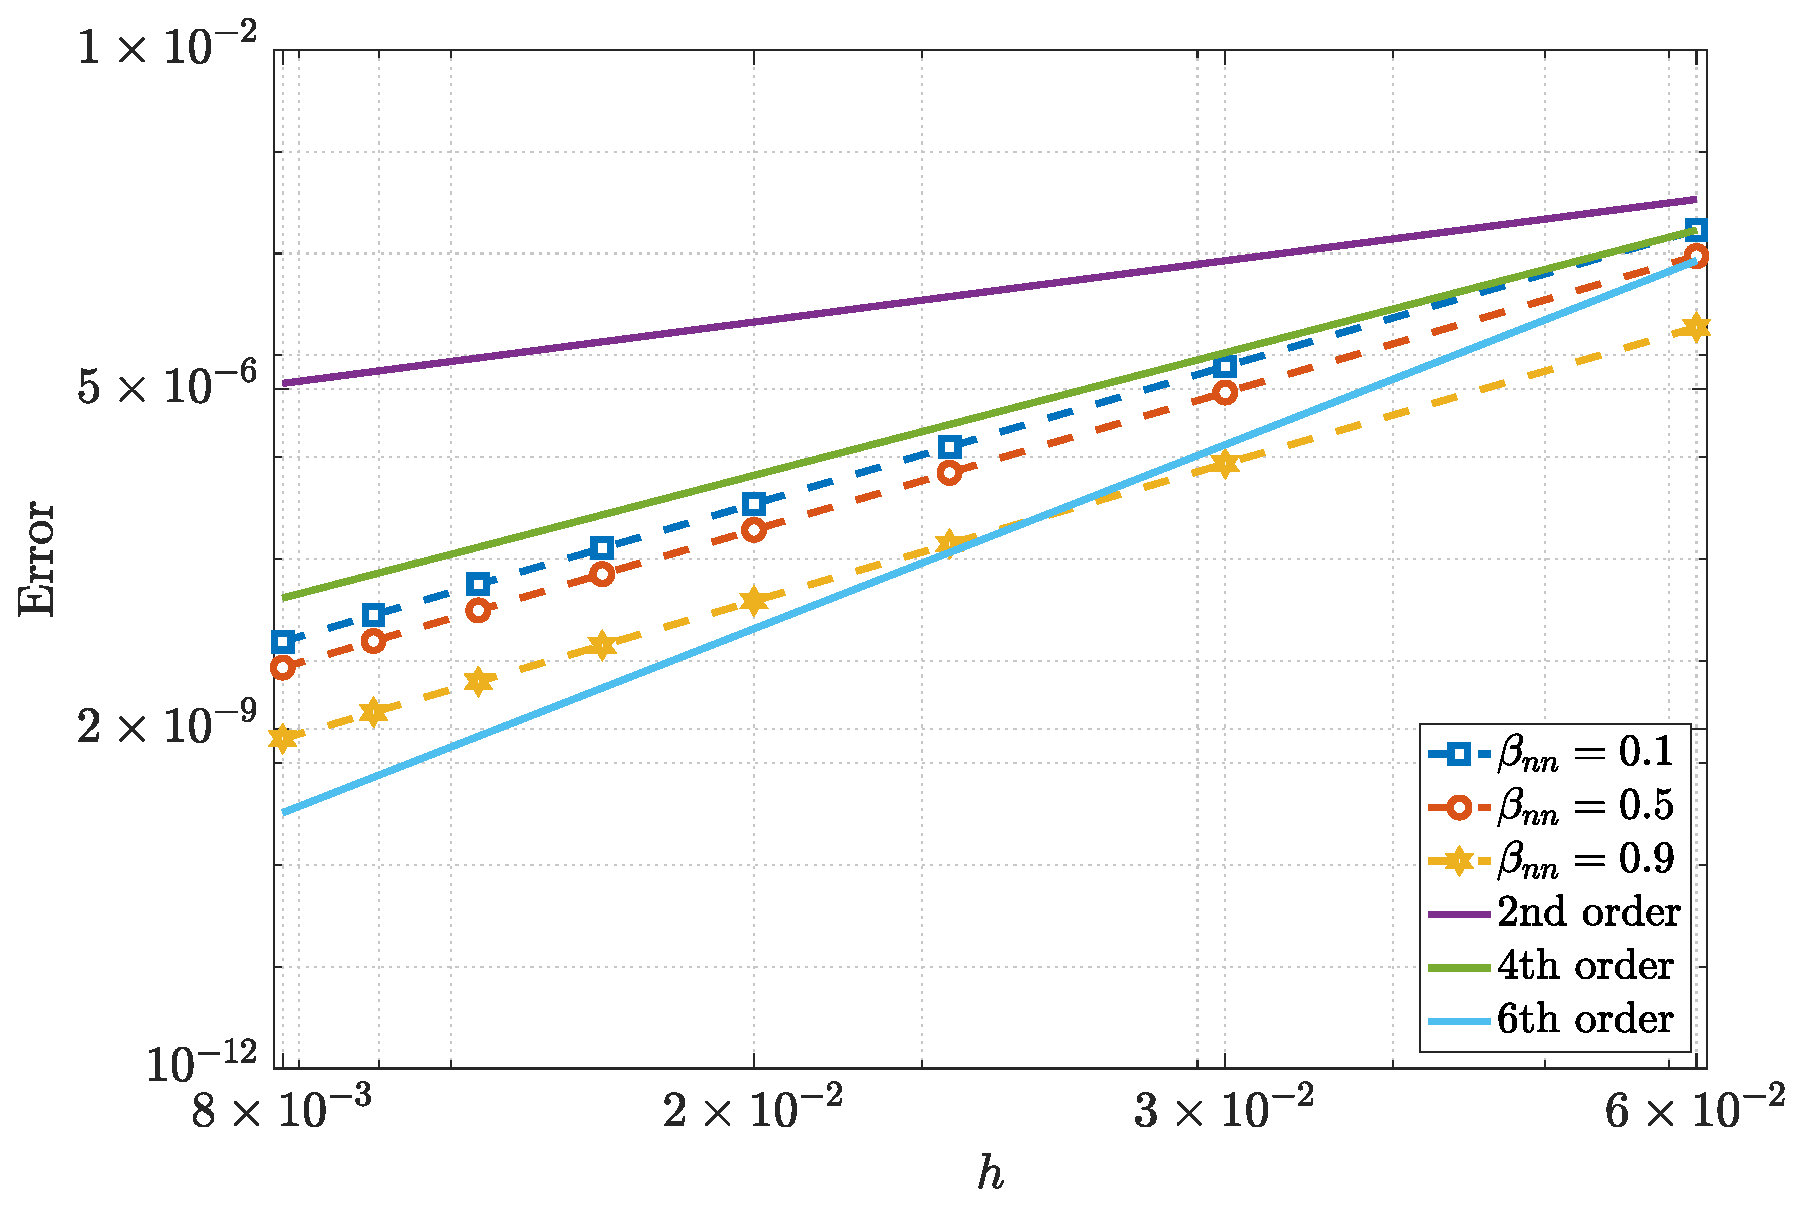
\includegraphics[width=\textwidth]{Figures/NormErr_2nd_Re_100_Wi_1_epsilon_0_xi_0_alphaG_0_Dt_1e-06_at_0.05_tipsim_1_MMS_12_Txy.eps}
        \captionof{subfigure}{$\overline{T_{xy}}$}
        \label{lptt_txy_Case11}
    \end{minipage}
    \hfill
    \begin{minipage}{0.325\textwidth}
        \centering
        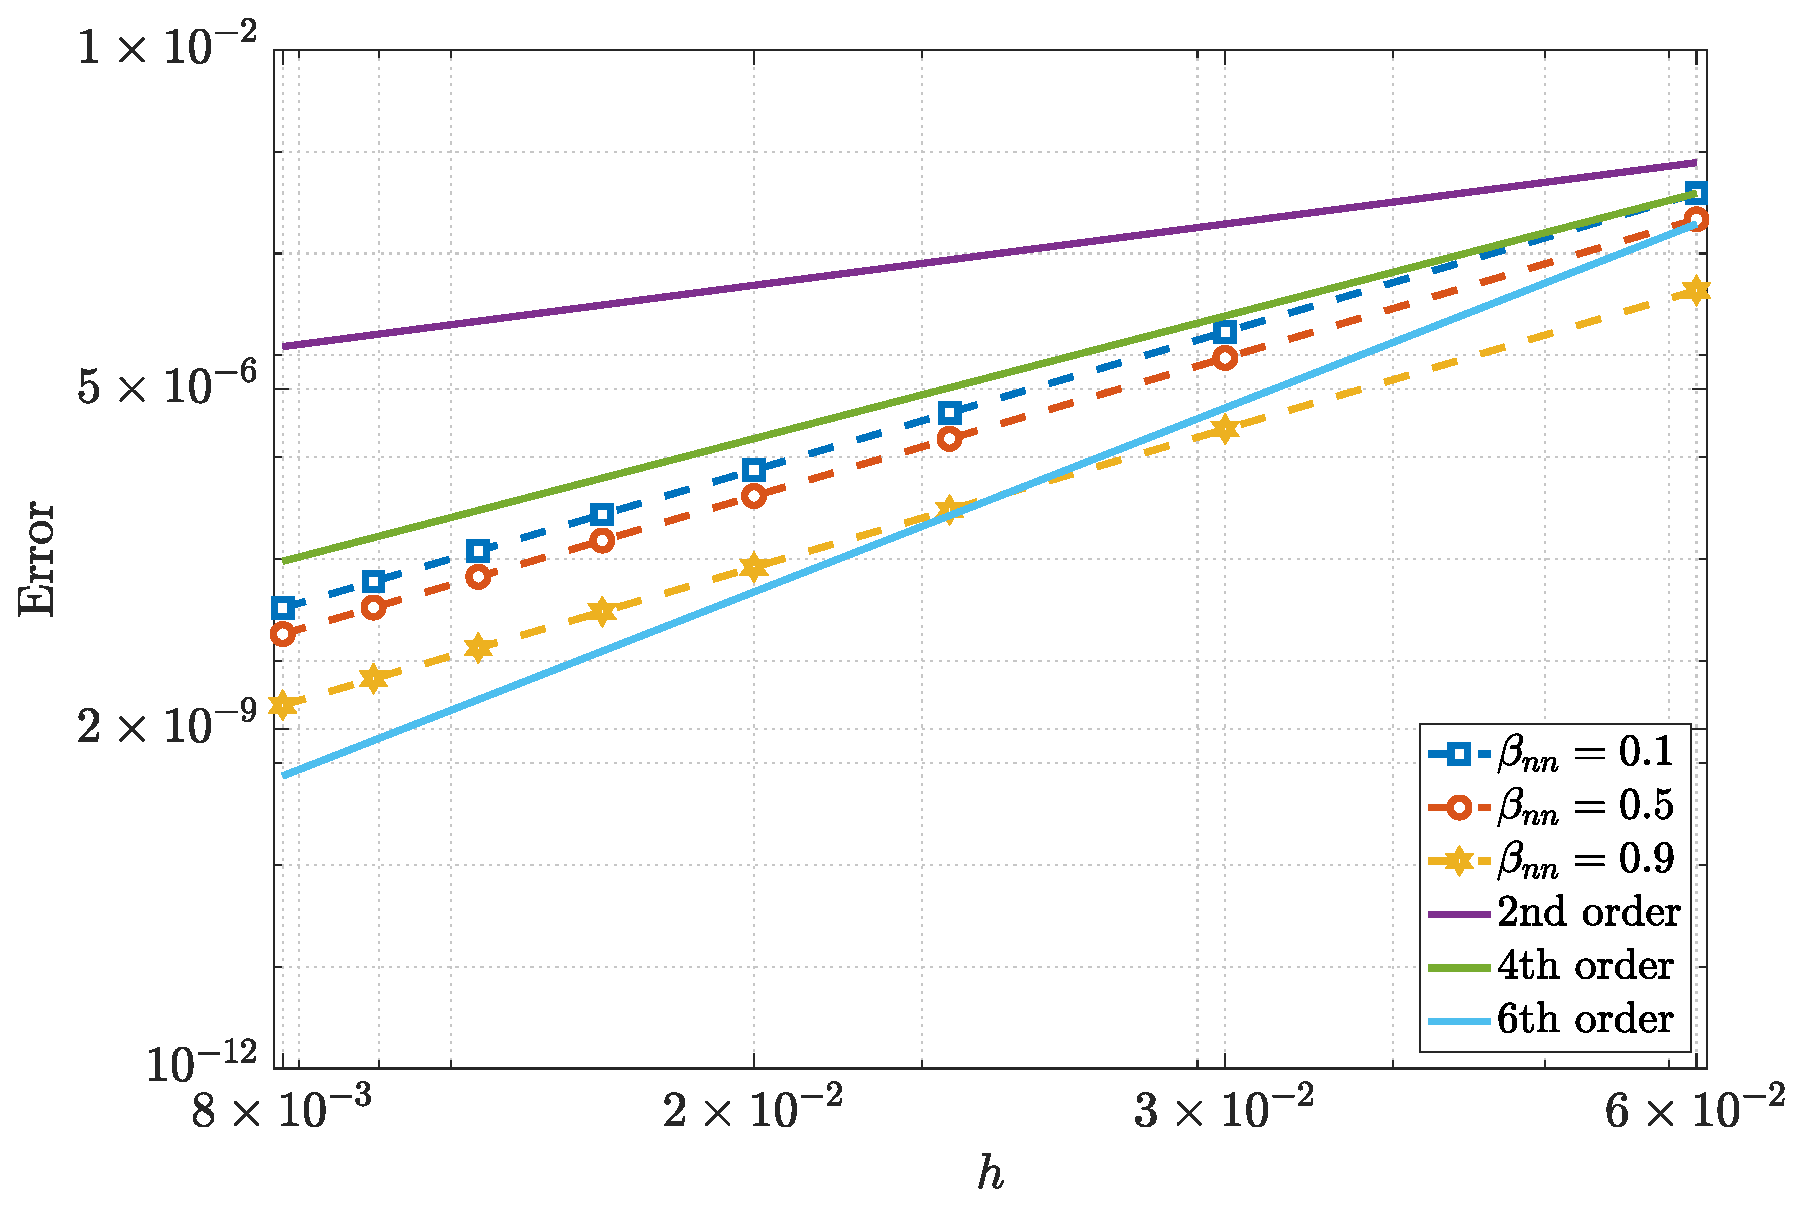
\includegraphics[width=\textwidth]{Figures/NormErr_2nd_Re_100_Wi_1_epsilon_0_xi_0_alphaG_0_Dt_1e-06_at_0.05_tipsim_1_MMS_12_Tyy.eps}
        \captionof{subfigure}{$\overline{T_{yy}}$}
        \label{lptt_tyy_Case11}
    \end{minipage}
\end{frame}

%%%%%%%%%%%%%%%%%%%%%%%%%%%%%%%%%%%%%%%%%%%%%%%%%%%%%%%%%%%%%%
\subsection{Considerações finais}
%%%%%%%%%%%%%%%%%%%%%%%%%%%%%%%%%%%%%%%%%%%%%%%%%%%%%%%%%%%%%%
%%%%%%%%%%%%%%%%%%%%%%%%%%%%%%%%%%%%%%%%%%%%%%%%%%%%%%%%%%%%%%

\begin{frame}{Conclusões}
\begin{itemize}
    \item O estudo reforça a eficácia dos métodos numéricos na simulação de fluidos viscoelásticos;
    \item Simulações para diversos números de Reynolds ($Re$) e Weissenberg ($Wi$), além de razões de viscosidade do solvente ($\beta_{nn}$), validaram a robustez dos modelos;
    \item O modelo UCM apresentou precisão elevada para fenômenos de elasticidade em malhas refinadas;
    \item O modelo LPTT demonstrou estabilidade e precisão para diferentes valores do parâmetro $\epsilon$;
    \item Fluidos Newtonianos ($\beta_{nn}=1$) atingiram erros próximos à precisão de máquina, validando os esquemas numéricos;
    \item O modelo Oldroyd-B mostrou-se robusto e preciso, enquanto o modelo Giesekus manteve estabilidade para valores de $\alpha_G$ variando entre 0.1 e 0.5;
    \item O Método das Soluções Manufaturadas se mostrou crucial para a verificação de códigos numéricos;
    \item Os resultados sustentam a aplicação dos modelos UCM, LPTT, Oldroyd-B e Giesekus em cenários complexos de escoamento;
\end{itemize}
\end{frame}

%%%%%%%%%%%%%%%%%%%%%%%%%%%%%%%%%%%%%%%%%%%%%%%%%%%%%%%%%%%%%%
\begin{frame}{Considerações finais e trabalhos futuros}
\begin{itemize}
    \item \textbf{SILVA, A. T. G. et al.} Validation of HiG-Flow Software for Simulating Two-Phase Flows with a 3D Geometric Volume of Fluid Algorithm. \textit{Mathematics}, v. 11, n. 18, p. 3900, 2023. 
\end{itemize}
\end{frame}